\documentclass[a4paper,12pt]{report}

\usepackage[utf8]{inputenc}
\usepackage[spanish]{babel}
\usepackage[pdftex]{graphicx}
\usepackage{ifpdf}
\usepackage{appendix}
\usepackage{listings}
\usepackage[colorlinks, citecolor=black, filecolor=black, linkcolor=black, urlcolor=black]{hyperref}
\usepackage{subfigure}
\usepackage{tikz}
\usetikzlibrary{shapes,snakes}
\usepackage{bookmark}
\usepackage[chapter]{algorithm}
\usepackage{algorithmic}

\usepackage{color}
\usepackage{textcomp}
\usepackage{lscape}
\definecolor{listinggray}{gray}{0.9}
\definecolor{lbcolor}{rgb}{0.95,0.95,0.95}
\lstset{
    backgroundcolor=\color{lbcolor},
    tabsize=4,
    rulecolor=,
    language=matlab,
        basicstyle=\scriptsize,
        upquote=true,
        aboveskip={1.5\baselineskip},
        columns=fixed,
        showstringspaces=false,
        extendedchars=true,
        breaklines=true,
        prebreak = \raisebox{0ex}[0ex][0ex]{\ensuremath{\hookleftarrow}},
        frame=single,
        showtabs=false,
        showspaces=false,
        showstringspaces=false,
        identifierstyle=\ttfamily,
        keywordstyle=\color[rgb]{0.1,0.1,0.6}\bfseries,
        commentstyle=\color[rgb]{0.133,0.545,0.133},
        stringstyle=\color[rgb]{0.627,0.126,0.941},
}


% Definitions
\def\fud {\textbf{\textit{FuD}}}
\def\fude {\textbf{\textit{FuDePAN}}}
\def\rc {\textbf{\textit{RecAbs}}}
\def\cpp {\textbf{\textit{C++}}}
\def\ana {\textbf{\textit{Ana}}}

% Tools
\def\doxy {\textbf{\textit{Doxygen}}}
\def\gc {\textbf{\textit{GoogleCode}}}
\def\uml {\textbf{\textit{UML}}}
\def\linux {\textbf{\textit{GNU/Linux}}}
\def\unix {\textbf{\textit{UNIX}}}
\def\make {\textbf{\textit{make}}}
\def\cmake {\textbf{\textit{CMake}}}
\def\autotools {\textbf{\textit{Autotools}}}

% Commands
\newcommand{\HRule}{\rule{\linewidth}{0.5mm}}
\renewcommand{\appendixname}{Apéndices}
\renewcommand{\appendixtocname}{Apéndices}
\renewcommand{\appendixpagename}{Apéndices}

%Headers
\usepackage{fancyhdr}
\pagestyle{fancy}
\fancyhf{}
\fancyhead[R]{\bfseries\thepage}
\fancyhead[L]{\nouppercase{\textsc{\rightmark}}}

\begin{document}

	\pagenumbering{roman}

    %Title
    \begin{titlepage}
        \begin{center}

            %Escudos
            \begin{minipage}{0.45\textwidth}
                \begin{center}
                    %Escudo UNRC
                    
\includegraphics[width=60pt,height=90.5pt]{images/unrc.jpg}\\
                    \begin{scriptsize}
                        \textsc{Universidad Nacional de Río Cuarto} \\
                    \end{scriptsize}
                    \vfill
                    \begin{tiny}
                        \textsc{Fac. de Cs. Exactas, Fco-Qcas y Naturales} \\
                        \textsc{Departamento de Computación} \\[1cm]    
                    \end{tiny}
                \end{center}
            \end{minipage}
            \begin{minipage}{0.45\textwidth}
                \begin{center}
                    %Escudo FuDePAN
                    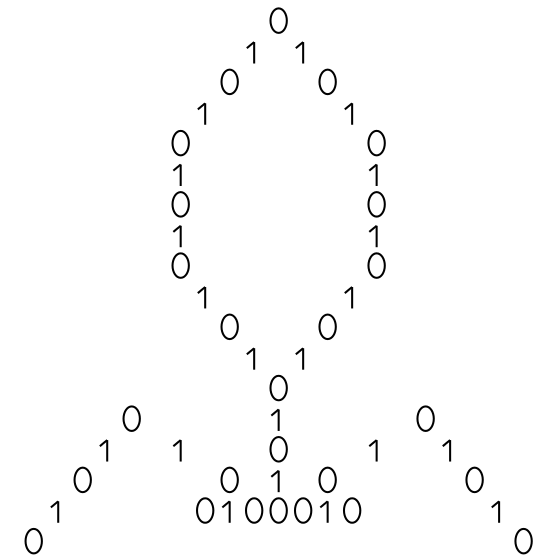
\includegraphics[width=90pt,height=90pt]{images/fudepan.png}\\
                    \vfill
                    \begin{scriptsize}
                        \textsc{FuDePAN} \\
                    \end{scriptsize}
                    \begin{tiny}
                        \textsc{Fundación para el Desarrollo de la Programación en Ácidos Nucleicos} \\[1cm]    
                    \end{tiny}
                \end{center}
            \end{minipage}

            \vspace{2cm}
            
            \textsc{\Large{Trabajo Final}}\\
            \textsc{Licenciatura en Ciencias de la Computación}\\
            
            \HRule\\[0.1cm]
            \textbf{\huge{RecAbs}\\[0.3cm]
                    \Large Abstracción de distribución de procesos recursivos implementada sobre FuD.}\\[0.1cm]
            \HRule\\[0.4cm]

            \vspace{1cm}

            \begin{large}
                \center{\small{\textsc{Autores}}}\\
                \textbf{Bessone}, Mariano José\\
                \textbf{Bringas}, Emanuel César
            \end{large}            
                
            \vspace{1cm}
            
            \begin{minipage}{0.4\textwidth}
                \begin{center}
                    \center{\small{\textsc{Director}}} \\
                    \large{\textbf{Biset}, Guillermo}
                \end{center}
            \end{minipage}
            \begin{minipage}{0.4\textwidth}
                \begin{flushright} 
                \center{\small{\textsc{Co-Director}}} \\
                \large{\textbf{Gutson}, Daniel}
                \end{flushright}
            \end{minipage}

            \vfill
            {\large 2 de Diciembre de 2011}
            
        \end{center}

    \end{titlepage}
    
    \begin{abstract}

        El procesamiento de grandes conjuntos de datos es un tema importante en Ciencias de la Computación; mucha información es
        inherentemente difícil de comprimir y, además, los recursos para procesar estas cantidades de datos usualmente es muy costoso.
        Existen muchas herramientas para lograrlo por medio de alguna forma de computación distribuida.
        
        Este trabajo provee un panorama general sobre el diseño y la implementación de una librería que brinda soporte para construir
        soluciones a problemas específicos recurrentes de la bioinformática. A su vez, este trabajo extiende el framework de distribución
        \fud{}, el cuál nos facilita la implementación de una solución distribuida del problema a resolver. Concretamente se trata de una
        capa de abstracción que permite desarrollar soluciones recursivas sin tener que lidiar con problemas comunes en la implementación
        de algoritmos distribuidos.

        El alcance de esta abstracción abarca a todos los problemas cuya solución recursiva no tenga dependencia de datos entre los nodos
        del árbol de recursión.

    \end{abstract}

    \newpage
\chapter*{Agradecimientos}

El presente trabajo fue fruto de un esfuerzo en el cuál, directa o indirectamente, participaron varias personas leyendo, opinando,
corrigiendo, apoyando y motivando en los distintos momentos que atravesamos en el desarrollo del mismo. Queremos agradecerles a todos ellos
por cuanto han hecho por nosotros para que este trabajo saliera adelante de la mejor manera posible.\\

En primer lugar, queremos agradecer especialmente a los dos directores de esta tesis: Daniel Gutson y Guillermo Biset, los mentores de este
proyecto y quienes confiaron en nosotros para que lo llevemos adelante. Estamos muy agradecidos por su generosidad al brindarnos la
oportunidad de recurrir a su capacidad y experiencia científica en un marco de confianza, afecto y amistad, fundamentales para la concreción
de este trabajo.\\

A los autores del proyecto \emph{CombEng}, Diego Díaz y Favio Bettiol por un constante feedback de nuestro proyecto que nos brindó un
progreso constante con una mayor calidad. Su labor fue muy importante en nuestra etapa de test, su disposición a la hora de trabajar en
conjunto fue total. Esperamos haberles sido de tanta utilidad a ellos como lo han sido para nosotros.\\

A German Regis y Nazareno Aguirre por su buena voluntad para ayudarnos con las formalidades requeridas por la universidad que este trabajo
demandó.\\

Al Departamento de Computación y a su director, en su momento Nazareno, por facilitarnos las salas de máquinas para realizar pruebas a
escalas un poco mayores.\\

A cada uno de los que forman parte de la fundación \fude{}, por ser personas que, sin esperar nada a cambio, trabajan incansablemente sólo
por su compromiso y amor a la investigación.\\

Finalmente, y no por eso menos importante, sino todo lo contrario, queremos agradecerles muy especialmente a nuestras familias por habernos
apoyado incondicionalmente a lo largo de toda la carrera. Esperamos que este trabajo, y el logro que el mismo conlleva, sea una mínima
retribución a tantas cosas que ellos nos han brindado durante todos los años de estudio.\\

    \newpage

    %Index
    \tableofcontents
    \newpage
    
    %Figure index
	\listoffigures
	\newpage

    %Figure Tables
    \listoftables
    \newpage

	\pagenumbering{arabic}
	
    % Part I
    \part{Preliminares}
    \label{part:prelim}

    \chapter{Introducción}

La idea original de este proyecto nace de \fude{} (\textbf{Fu}ndación para el \textbf{De}sarrollo de la \textbf{P}rogramación en
\textbf{Á}cidos \textbf{N}ucleicos), organización sin fines de lucro que se dedica a la investigación y desarrollo en bioinformática,
aplicándola a problemas biológicos asociados a la salud humana. En esta fundación se utiliza a la computación para hacer simulaciones y
cálculos para, por ejemplo, mejorar vacunas, mejorar tratamientos contra enfermedades como el HIV, o el virus Junín, desarrollando y
utilizando herramientas informáticas y programación de avanzada.\\

La mayoría de los problemas que la fundación enfrenta diariamente son de gran complejidad, por lo que se requiere de altos recursos
computacionales para lograr tener resultados a corto plazo. Es por ello que existe el framework \fud\cite{clus09} para la distribución
automática de trabajos en nodos de cómputo, que permite mediante una simple reimplementación de proyectos ya desarrollados de manera
secuencial, obtener una versión paralelizada del mismo. De esta manera se logró obtener resultados confiables en un tiempo relativamente
corto.\\

Asimismo, se notó que muchos problemas bioinformáticos, corrientes y a futuro, son naturalmente solucionados usando recursión pero no había
una forma de agruparlos y facilitar su desarrollo. Por esta razón, surge la motivación de construir una implementación genérica a toda
solución recursiva como una capa más del framework.\\

Los objetivos planteados al comienzo del proyecto fueron los siguientes:
\begin{itemize}
    \item   Diseñar una abstracción que permita a cualquier programador de la fundación poder construir soluciones recursivas paralelizadas
            de una manera sencilla. Evitando así la dificultad que conlleva lidiar con problemas inherentes a la programación paralela.
    \item   Construir esta abstracción como una aplicación particular de \fud{} que abarque toda solución recursiva de un problema que no
            requiera \textit{backtracking}.
    \item   Refactorizar \fud{} con el fin de aportar funcionalidades de interactividad entre cliente y servidor, lo cuál es necesario para
            el desarrollo de \rc. Este rediseño debe respetar los principios originales del framework, para que toda aplicación que lo use
            lo siga haciendo sin modificación alguna en la nueva versión.
    \item   En ambas implementaciones procurar cumplir con los requisitos de calidad y performance en cuánto a código y diseño.
\end{itemize}

Este documento proporciona una visión general sobre el diseño y detalles de implementación de los puntos mencionados anteriormente, junto
con ejemplos de su uso y algunos resultados estadísticos sobre el rendimiento de aplicaciones.\\

El informe se divide en 4 partes. La Parte \ref{part:prelim} incluye una introducción a este trabajo, un capítulo con el marco teórico para
facilitar la lectura de este documento y otro con la metodología de trabajo utilizada para llevar a cabo el proyecto.

La Parte \ref{part:recabs} contiene todo lo relacionado con \rc, a partir del enunciado del problema y el enfoque de la solución tomado, el
lector encontrará detalles acerca del diseño e implementación de la capa, junto con ejemplos sencillos de su uso.

La Parte \ref{part:refactorin_fud} introduce el problema de montado \rc/\fud, seguido de la refactorización del framework, con el fin de
acoplar la capa de abstracción de distribución de procesos recursivos sobre éste.

Finalmente, la Parte \ref{part:conclusion} brinda la conclusión sobre la tesis y un mapa de los trabajos que quedan por hacer.

En la parte de apéndices, hay dos reportes de métricas de código generados automáticamente, tanto de \rc{} como de la refactorización de
\fud, y documentación sobre patrones de diseño utilizados en este proyecto.

    \chapter{Marco Teórico}
\label{chap:marco_teorico}

\section{Programación Paralela}

La computación paralela es una técnica de programación en la que muchas instrucciones se ejecutan
simultáneamente\cite{Lorin:1990:RHP:1011116.1011127}. Se basa en el principio de que los problemas grandes se pueden dividir en partes más
pequeñas que pueden resolverse de forma concurrente (``en paralelo''). El término \textit{``Parallel Computer''} es bastante amplio y admite
varias definiciones. En \cite{parallel} se encuentra la siguiente definición:

\begin{quote}
\textit{``Una computadora paralela es un conjunto de procesadores que son capaces de trabajar colaborativamente para resolver un problema
computacional. Esta definición es lo suficientemente amplia como para incluir supercomputadoras paralelas que tienen cientos o miles de
procesadores, redes, estaciones de trabajo y sistemas embebidos. Las computadoras paralelas son interesantes porque ellas ofrecen el
potencial de concentrar recursos computacionales (ya sea ancho de banda, procesadores, memoria, E/S, etc) sobre importantes problemas de
cálculo."}
\end{quote}

Sin embargo es posible clasificar las diferentes arquitecturas de computadoras con el fin de estudiar las propiedades de cada una. En la
siguiente subsección se mostrará un estándar académico e industrial sobre la taxonomía propuesta por Michael J. Flynn.

\subsection{Taxonomía de Flynn}

La taxonomía es una clasificación de arquitecturas de computadoras, propuestas por Michael J. Flynn en 1966 y publicada en 1972\cite{flynn}.
Las cuatro clasificaciones definidas se basan en el número de instrucciones concurrentes (control) y en los flujos de datos disponibles en
la arquitectura. Un flujo de instrucciones es el conjunto de instrucciones secuenciales que son ejecutadas por un único procesador, y un
flujo de datos es el flujo secuencial de datos requeridos por el flujo de instrucciones. Con estas consideraciones, Flynn clasifica a los
sistemas en cuatro categorías.

\begin{description}
	\item [Una instrucción, un dato (SISD)] : Computador secuencial que no explota el paralelismo en las instrucciones ni en flujos de
        datos. Ejemplos de arquitecturas SISD son las máquinas con uni-procesador o monoprocesador tradicionales como el PC o los antiguos
        \textit{mainframe}. En la figura \ref{sisd} se muestra un diagrama que ilustra esta arquitectura.
			
	\item [Una instrucción, múltiples datos (SIMD)] : Un computador que explota varios flujos de datos dentro de un único flujo de
        instrucciones para realizar operaciones que pueden ser paralelizadas de manera natural. Por ejemplo, un procesador vectorial. En la
        Figura \ref{simd} se muestra un diagrama que ilustra esta arquitectura.
	
	\item [Múltiples instrucciones, un dato (MISD)] : Poco común debido al hecho de que la efectividad de los múltiples flujos de
        instrucciones suelen precisar de múltiples flujos de datos. Sin embargo, este tipo se usa en situaciones de paralelismo redundante,
        como por ejemplo en navegación aérea, donde se necesitan varios sistemas de respaldo en caso de que uno falle. También se han
        propuesto algunas arquitecturas teóricas que hacen uso de MISD, pero ninguna llegó a producirse en masa. En la Figura \ref{misd} se
        muestra un diagrama que ilustra esta arquitectura.

	\item [Múltiples instrucciones, múltiples datos (MIMD)] : Varios procesadores autónomos que ejecutan simultáneamente instrucciones
        diferentes sobre datos diferentes. Los sistemas distribuidos suelen clasificarse como arquitecturas MIMD; bien sea explotando un
        único espacio compartido de memoria, o uno distribuido. En la Figura \ref{mimd} se muestra un diagrama que ilustra esta
        arquitectura.
\end{description}

\subsubsection{Otras clasificaciones}

La clasificación de Flynn ha demostrado funcionar bastante bien para la tipificación de sistemas, y se ha venido usando desde décadas por la
mayoría de los arquitectos de computadores. Sin embargo, los avances en tecnología y diferentes topologías, han llevado a sistemas que no
son tan fáciles de clasificar dentro de los 4 tipos de Flynn como lo son ``Single Program, Multiple Data" (SPMD) y ``Multiple Program
Multiple Data" (MPMD).
	
	\begin{figure}[ht]
		\centering
		\subfigure[Diagrama de SISD.]{
			\label{sisd}	
			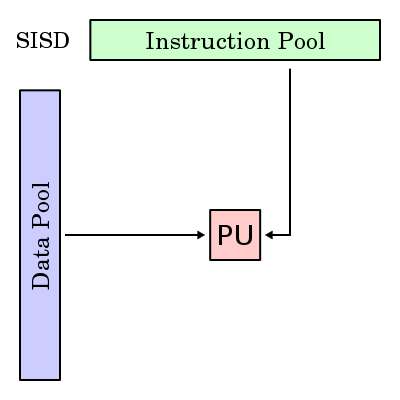
\includegraphics[width=150pt]{images/SISD.png}			
		}
		\subfigure[Diagrama de SIMD.]{
			\label{simd}	
			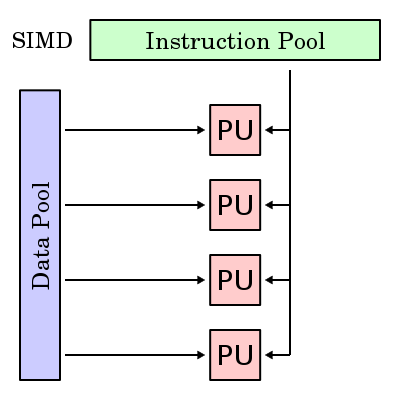
\includegraphics[width=150pt]{images/SIMD.png}			
		}
		\label{flynDiagram}
		\\
		\subfigure[Diagrama de MISD.]{
			\label{misd}	
			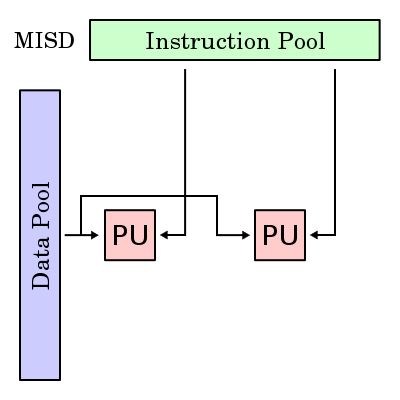
\includegraphics[width=150pt]{images/MISD.png}			
		}
		\subfigure[Diagrama de MIMD.]{
			\label{mimd}	
			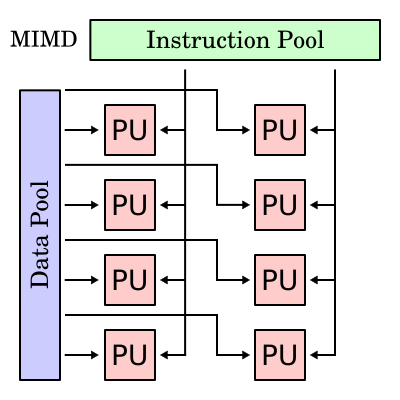
\includegraphics[width=150pt]{images/MIMD.png}			
		}
		\caption{Taxonomia de Flynn}
	\end{figure}	

\subsection{Resolución de problemas paralelos}

Cuando tenemos un problema que requiere una gran capacidad de cómputo, ya sea por una gran cantidad de datos de entrada o por una gran
complejidad en sus operaciones, podemos optar solucionarlo mediante el desarrollo de algoritmos paralelos. El primer paso para el diseño de
un algoritmo paralelo consiste en descomponer el problema principal en problemas más pequeños o subproblemas para que luego sean asignados a
cada procesador y puedan ser ejecutados de manera independiente y simultánea.

No siempre es una buena decisión partir de un algoritmo secuencial intentando ``paralelizar'' la aplicación, sino que en ciertas ocasiones
es necesario diseñar un nuevo algoritmo que, seguramente, será muy diferente al secuencial.
Entre las descomposiciones mas conocidas se encuentran:

    \begin{description}
     \item[Descomposición de dominio o paralelismo de datos] consiste en descomponer los datos de entrada de
un programa paralelo en porciones más pequeñas e indivisibles de tal manera que posean aproximadamente el mismo tamaño. Cada una de estas
porciones son asignadas a un procesador para su posterior ejecución. Se puede relacionar al paralelismo de datos con el modelo \textbf{SIMD}
ya que permite mantener un único flujo de instrucciones.
     \item[Descomposición funcional] se basa en la división del programa principal en subtareas mas pequeñas donde cada una de éstas son
asignadas y ejecutadas de manera independiente por cada procesador. En muchos casos, el número de subtareas obtenidas puede ser mayor a la
cantidad de procesadores con los que se cuenta. \\
Este tipo de descomposición se implementa siguiendo un paradigma maestro-esclavo donde existe un proceso maestro que se encarga de enviar
subtareas a los procesos  esclavos. Cuando uno de éstos últimos termina su computación, los resultados se envían al proceso maestro el cual
nuevamente le asigna una nueva subtarea a procesar. Se prosigue de ésta manera hasta agotar las subtareas pendientes.
    \end{description}

\subsection{Paradigmas de programación paralela}

Los paradigmas de programación no están totalmente ligados a las arquitecturas paralelas, pero si estrechamente relacionado. Podríamos decir
que cada arquitectura de computación paralelas justifica esta relación haciendo uso de dichos paradigmas. Es por eso que un determinado
paradigma puede ser más eficiente que otros al programar  sobre determinadas arquitecturas paralelas. Existen dos tipos de paradigmas
principalmente utilizados para la programación paralela:

    \begin{description}
     \item[Memoria compartida] Se ve a los programas como una colección de procesos que pueden acceder a variables locales y a variables
globales almacenadas en un espacio de memoria compartido entre las diversas unidades de procesamiento. Cada proceso accede a dicha memoria
compartida a través de lecturas asíncronas.\\
Este paradigma, como bien lo indica su nombre, es apropiado para el desarrollo de aplicaciones sobre arquitecturas de memoria compartida,
aunque también puede ser utilizado para el desarrollo de aplicaciones para arquitectura distribuida, simulando un espacio de memoria
compartido.
    \item[Paso de mensajes] es una técnica empleada para aportar sincronización entre procesos y permitir la exclusión mutua de manera
similar a como se hace con los semáforos, monitores, etc. Su principal característica es que no precisa de memoria compartida, por lo que es
muy importante en la programación de sistemas distribuidos. Los elementos principales que intervienen en el paso de mensajes son: el proceso
que envía, el que recibe y el mensaje.
    \end{description}

\subsection{Balanceo de carga}

Un aspecto fundamental que hay que tener en cuenta a la hora de desarrollar un programa paralelo es el \textit{balanceo de carga}.

Ésta es una metodología para distribuir equitativamente los trabajos a través de múltiples computadoras, clusters, redes de trabajos,
discos, o todo aquello que conforme el sistema paralelo utilizado, de tal manera que se pueda asegurar el uso y distribución óptima de los
recursos y poder maximizar la salida, minimizar el tiempo de respuesta y evitar sobrecargas. El servicio de \textit{balanceo de carga}
usualmente lo proveen programas dedicados o dispositivos de hardware\cite{buyya99}.

El equilibrio de carga es comúnmente utilizado para realizar comunicaciones internas en clusters o para implementar algoritmos de
planificación en sistemas operativos.

\subsection{Etapas de diseño}

Las etapas de diseño de aplicaciones paralelas podrían resumirse entonces como sigue:

\begin{itemize}
 \item Identificar el trabajo que puede realizarse en paralelo.
 \item Diseñar la división y unificación del trabajo y datos entre los procesadores.
 \item Resolver el acceso a los datos, las comunicaciones entre procesos y las sincronizaciones.
 \item Asignar recursos de cómputo a los procesos que se ejecutarán en paralelo.
\end{itemize}


\section{FuD}
\label{sec:fud}

FuD es un framework para la distribución de procesos, o bien, un framework para la implementación de aplicaciones distribuidas\cite{clus09}.
FuD no depende del problema a implementar y no fuerza a usar un modelo de comunicación particular ni restringue a cualquier disposición de
nodos de procesamiento con que se cuente. Por lo tanto, las aplicaciones pueden ejecutarse en cluters heterogéneos y dinámicos.

Este framework provée una base para pequeños y medianos proyectos que necesitan manejar grandes conjuntos de datos y particularmente con
gran demanda de independencia de procesamiento con bajos requerimientos de comunicación.

FuD se divide entre aplicación servidor y cliente organizado en tres capas, cada una con una responsabilidad clara. La comunicación entre
las mismas es limitada estrictamente, cada una ellas tiene solo un punto de comunicación.
Las capas y sus responsabilidades son las siguientes:

\begin{figure}[!ht]
\begin{center}
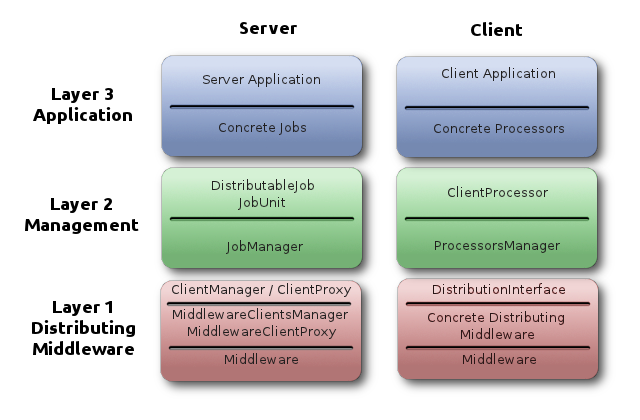
\includegraphics [width=300pt]{images/FuD-AbstractLayers.png}
\label{fud_layers}
\end{center}
\caption{Diseño de FuD.}
\label{fud-layers}
\end{figure}

\begin{description}
	\item[Capa de aplicación (L3)] Esta capa proporciona componentes que describen el problema a resolver, tanto en lo que respecta a los
            algoritmos y los datos utilizados. En el lado del servidor reside la aplicación principal, la distribución de la estrategia y
            los componentes de datos. En el lado del cliente, sólo una aplicación de los métodos para hacer los cálculos correspondientes en
            las unidades de trabajo.	
	\item[Capa de manejo de trabajo (L2)] La responsabilidad de esta capa es manejar los trabajos, que pueden ser divisibles o atómicos.
            Registran trabajos distribuibles concretos y genera unidades de trabajo que son pasados a la capa subyacente para su
            procesamiento y una vez obtenido el resultado correspondiente informa a la capa superior la finalizacion del trabajo y la
            comunicación de los resultados.
	\item[Capa de comunicación (L1)] En el lado del servidor, el registro y estado de clientes se maneja en esta capa. En ambos lados hay
            una subcapa constante que son las interfaces del middelware mientras que las implementaciones concretas estan en otra subcapa
            variable (Por ejemplo, BOINC\footnote{Berkeley Open Infrastructure for Network Computing. http://boinc.berkeley.edu} o
            MPI\footnote{An API specification for communication: http://www.mpi-forum.org/docs} ).
			
\end{description}


\section{Recursión}

En el sentido más amplio de la palabra, \textbf{recursión} (o recurrencia, o recursividad) es la forma en la cual se especifica un proceso
basado en su propia definición. Dicho de otra forma, es el proceso de repetir cosas de una manera \textit{auto-similar}, propiedad de un
objeto en el que el todo es exacta o aproximadamente similar a una parte de sí mismo.
La recursión, en ciencias de la computación, es un método para resolver problemas computacionales donde la solución depende de las
soluciones de instancias más pequeñas del mismo problema\cite{conmath94}.

\begin{quote}
    \textit{``El poder de la recursión, evidentemente, radica en la posibilidad de definir un conjunto infinito de objetos con una
    declaración finita. De la misma manera, un número infinito de cálculos puede ser descrito por un programa recursivo finito, aunque este
    programa no contenga repeticiones explícitas.''}\cite{algdatpro76}
\end{quote}

En computación el artefacto de la recursión es el \textit{algoritmo recursivo}. Estos algoritmos tienen una importancia fundamental e
indispensable en prácticamente todas las áreas en el campo de la informática. Para muchos problemas, el uso de la recursividad permite
resolver problemas complejos mediante algoritmos concisos, fáciles de comprender y eficientes (desde el punto de vista algorítmico).

En su forma más simple, la recursividad es el proceso de dividir el problema en uno o más subproblemas, que son idénticos en estructura al
problema original y luego la combinación de las soluciones a estos subproblemas para obtener la solución al problema original. Pero en
general podemos identificar tres casos especiales de esta técnica de diseño:
\begin{enumerate}
    \item   \textbf{Inducción} (o tail recursion).
    \item   Subproblemas sin superposición, usando \textbf{divide \& conquer}.
    \item   Subproblemas con superposición con redundantes invocaciones a subproblemas, lo que permite intercambiar espacio por tiempo. Se
            usa la técnica de \textbf{programación dinámica}.
\end{enumerate}

Los casos con números superiores incluyen a los de números más bajos. En los primeros dos casos no se requiere espacio adicional para llegar
a la solución. La tercera clase, sin embargo, da la posibilidad de solucionar eficientemente muchos problemas que a primera vista parecen
consumir mucho tiempo, debido a los repetidos cómputos que se realizan sin esta técnica\cite{alsuwaiyel98}.

Cabe aclarar que, el alcance de este trabajo abarca sólo las dos primeras técnicas. Aún así, el último caso es desarrollado también, a
modo de ejemplo de técnica no aplicable en este proyecto.

\subsection{Inducción}

En esta sección veremos a la inducción como una técnica para el desarrollo de algoritmos, en pocas palabras: la idea de inducción en pruebas
matemáticas es llevada al plano computacional obteniendo, así, diseño de algoritmos eficientes.

Para entender esta técnica vamos a considerar un problema de tamaño $n$, el cual normalmente representa el número de objetos (o partes) de
un problema. Cuando buscamos una solución para un problema en particular, algunas veces es más fácil comenzar solucionándolo con un
parámetro mas chico, $n-1$, $n/2$, etc, y extender esta solución para incluir los $n$ objetos. Esta forma de resolver problemas esta basada
en la muy conocida técnica de prueba: \textbf{inducción matemática}. Básicamente, dado un problema de parámetro $n$, diseñar un algoritmo
por inducción esta basado en el hecho de que si sabemos resolver el problema cuando tiene un parámetro menor a $n$, esto es llamado la
\textit{hipótesis inductiva}, entonces nuestra tarea se reduce a extender la solución para incluir a todos los objetos, llegando así al
parámetro $n$.

Este método puede ser generalizado para alcanzar todas las técnicas de diseño de algoritmos recursivos incluyendo las de divide \& conquer y
programación dinámica, sin embargo, estas tienen diferentes características que serán vistas en las próximas dos secciones.

En resumen, podemos decir que otras técnicas de programación tienen una estrecha relación con la \textit{inducción} pero vamos a darle ese
nombre sólo a los algoritmos que usen estrategias basadas \textit{claramente} de inducción matemática, a aquellos algoritmos que usualmente
sólo tienen una llamada recursiva, y son comúnmente llamados \textit{tail recursion}. Estos, en la mayoría de los casos, pueden ser
convenientemente convertidos a algoritmos iterativos.

Una ventaja de esta técnica (y de todos los algoritmos recursivos en general) es que la prueba de corrección del algoritmo diseñado es
naturalmente visto como su descripción, y por lo tanto una simple prueba inductiva puede ser fácilmente construida si se
desea\cite{alsuwaiyel98}.


\subsection{Divide \& Conquer} \label{divideandconquer}

Como dijimos anteriormente, podemos encontrar casos especiales de esta técnica de diseño llamada recursión, y una de ellas es la de resolver
recursivamente problemas que tienen subproblemas sin superposición entre ellos, o sea, problemas en los que no se comparten mismas
soluciones para subproblemas generados. Esto es a lo que se le llama en inglés \textit{Nonoverlapping subproblems}, y este tipo de problemas
puede ser naturalmente resuelto por la conocida técnica de \textbf{Divide \& Conquer}\cite{levitin06}.

\begin{quote}
    \begin{flushright}
        \textit{``Divide et vinces'' (Divide y vencerás),\\Julio César.}
    \end{flushright}
\end{quote}

Esta frase célebre nos conduce a una buena estrategia recursiva para resolver problemas que se puedan dividir en subproblemas más
sencillos.

% Alsuwaiyel page 175
En ciencias de la computación, el término ``\textit{divide y vencerás}'' hace referencia a una poderosa técnica de diseño de
algoritmos utilizada para resolver una amplia variedad de problemas. En su forma más simple, un algoritmo \textit{divide \& conquer} divide
un problema en una serie de subproblemas (en la mayoría de los casos 2), luego resuelve de forma recursiva cada uno de ellos por separado, y
por último, combina las soluciones de los subproblemas para obtener la solución al problema original\cite{alsuwaiyel98}.\\

% Cormen page 29
Según el libro \cite{cormen09}, el paradigma \textit{divide \& conquer} involucra tres pasos en cada nivel de la recursión:
\begin{itemize}
    \item   \textbf{Dividir} el problema en un numero de subproblemas.
    \item   \textbf{Conquistar} los subproblemas, resolviéndolos recursivamente. Por más que el tamaño de los subproblemas sean lo
            suficientemente pequeños, sólo se deben resolver de una manera directa.
    \item   \textbf{Combinar} las soluciones de los subproblemas en la solución del problema original.\\
\end{itemize}

% Skiena page 147
\begin{flushleft}
    \textbf{Relación de recurrencia}
\end{flushleft}
 
Como sabemos, una relación de recurrencia, que pasado al plano computacional se puede ver como un algoritmo recursivo, es una ecuación
que está definida en términos de ella misma. Por ejemplo, los \textit{números de Fibonacci}\cite{sigler03} están descritos por la relación
de recurrencia $F_n = F_{n-1} + F_{n-2}$. Esencialmente, las relaciones de recurrencia proporcionan una manera de analizar las estructuras
recursivas, tales como los algoritmos.

La función para el tiempo de ejecución de un algoritmo \textit{divide \& conquer} esta basado en los tres pasos del paradigma básico,
mencionados anteriormente. Sea $T(n)$ el tiempo en que se ejecuta un problema de tamaño $n$. Si el tamaño del problema es lo suficientemente
pequeño, como por ejemplo $n \leq c$ para una constante $c$, la solución trivial toma un tiempo constante, denotado por $\Theta(1)$.
Supongamos que la división del problema se obtiene en $a$ subproblemas, y cada uno de ellos es $1/b$ el tamaño del original. Si tomamos a
$D(n)$ como el tiempo para dividir el problema en subproblemas y que $C(n)$ es el tiempo para combinar las soluciones de los subproblemas en
la solución del problema original, obtenemos la siguiente función $T(n)$:\\

\[ T(n) = \left\{ \begin{array}{ll}
         \Theta(1) & \mbox{if $n \leq c$ },\\
         aT(n/b) + D(n) + C(n) & \mbox{otherwise} \end{array} \right.
\]

La figura \ref{recursion_tree} muestra el árbol de recursión asociado con un típico $T(n)$ de un algoritmo divide y vencerás. Cada problema
de tamaño $n$ se descompone en un problema de tamaño $n/b$. Cada subproblema de tamaño $k$ toma un tiempo $O(f(k))$ para ocuparse de su
interior, entre la partición y luego su fusión. El tiempo total para el algoritmo es la suma de los costos internos, mas el
\textit{overhead} de construir el árbol de recursión. La altura de este árbol es $h = \log_b n$ y el número de hojas $a^h = a^{\log_b n}$,
que se simplifica en $n^{\log_b a}$ con un poco de manipulación algebraica.

\begin{figure}[!ht]
\begin{center}
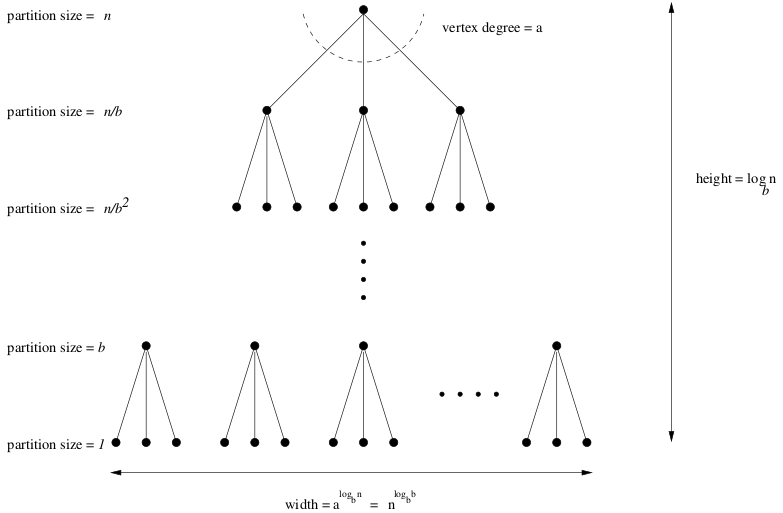
\includegraphics[width=400pt,height=262pt]{images/recursion-tree.png}
\end{center}
\caption{Árbol de recursión resultante de descomponer cada problema de tamaño $n$ en subproblemas de tamaño $n/b$.}
\label{recursion_tree}
\end{figure}

% Ejemplo Fibonacci
Siguiendo con el ejemplo de la sucesión de Fibonacci, su definición recursiva sería la siguiente:
\begin{equation} \label{def-fib} \end{equation}
\[ Fib(n) = \left\{ \begin{array}{ll}
         1 & \mbox{if $n = 1$ or $n = 2$ },\\
         Fib(n-1) + Fib(n-2) & \mbox{if $n \geq 3$} \end{array} \right.
\]
Dada esta definición, es fácil escribir un programa recursivo para computar el número de Fibonacci $N$.
Esta versión recursiva tiene la ventaja de ser concisa, fácil de escribir, de depurar y, sobre todo, su abstracción es clara. Hay una clase
rica de algoritmos recursivos y, en muchos casos, un complejo algoritmo se puede escribir sucintamente con el uso de la recursividad.\\

% Skiena page 147
Problemas más pequeños nos permiten centrarnos en detalles que se pierden cuando se está estudiando al problema por completo. Un algoritmo
recursivo comienza a ser evidente cuando se puede dividir el problema en partes más pequeñas del mismo tipo de problema. Para un
procesamiento paralelo eficaz se requiere una descomposición de trabajos en, al menos, tantas tareas como procesadores, y este es un tema
cada vez más importante debido al advenimiento de \textbf{cluster computing} y los procesadores multinúcleo\cite{skiena08}.

% Alsuwaiyel page 155
Como conclusión vemos que, las ventajas más atractivas de algoritmos divide \& conquer son: la concisión, la facilidad de comprensión y
ejecución, y lo más importante es que se pueden hacer, de manera fácil, pruebas de inducción para demostrar la corrección de este tipo de
algoritmos.


\subsection{Programación Dinámica}

% Common knowledge and wikipedia
Como bien sabemos, la \textit{programación dinámica} es una de las técnicas de programación mas usadas para resolver problemas en los
cuales sus subproblemas no son independientes, o sea, que \textit{comparten} soluciones comunes, a lo cual llamamos \textit{subproblemas
superpuestos}. Cada subproblema se resuelve sólo una vez y se guarda la respuesta en una tabla, evitando así el trabajo de volver a
calcular la respuesta cada vez que se encuentra el subproblema. 

La programación dinámica es típicamente utilizada en \textit{problemas de optimización}. En este tipo de problemas puede haber muchas
soluciones posibles. Cada solución tiene un valor, y queremos encontrar una solución con el valor óptimo (mínimo o máximo). Llamamos
a esta solución \textbf{una} solución óptima al problema, a diferencia de \textbf{la} solución óptima, ya que puede haber varias soluciones
que permitan alcanzar el valor óptimo\cite{cormen09}.

Más específicamente, la programación dinámica es aplicada a problemas con \textit{subestructura óptima}. Un problema se dice que tiene
subestructura óptima si una solución óptima se puede construir de manera eficiente de las soluciones óptimas para sus subproblemas. Por
ejemplo, el camino más corto entre dos vértices de un grafo se puede encontrar calculando primero el camino más corto al objetivo desde
todos los vértices adyacentes al de partida, y después usando estas soluciones para elegir el mejor camino de todos
ellos\cite{bellman10}.\\

% Alsuwaiyel page 155
Pero... ¿Qué tiene que ver recursión con programación dinámica?
% 
En esta técnica de diseño, la recursividad es solamente utilizada para modelar la solución del problema, como enfoque de la solución. Luego,
este modelo recursivo se convierte, en la mayoría de los casos, en un eficiente algoritmo iterativo en contraste con las redundantes
llamadas que hace la recursión\cite{alsuwaiyel98}.

% Skiena page 285
De hecho, la programación dinámica es una técnica eficiente para la implementación de un algoritmo recursivo mediante el almacenamiento de
resultados parciales. El truco está en ver si el \textit{ingenuo} algoritmo recursivo calcula el mismo subproblema una, y otra, y otra vez.
Si es así, el almacenamiento de la respuesta para cada subproblema en una tabla para luego buscar, en lugar de volver a calcular, puede dar
lugar a un algoritmo eficiente. Comienza con un algoritmo o definición recursiva. Sólo una vez que tenemos un algoritmo recursivo correcto,
ahora lo que nos preocupa es acelerarlo mediante el uso de una matriz de resultados.

La programación dinámica es generalmente el método adecuado para problemas de optimización combinatoria en objetos que tienen inherentemente
un orden de izquierda a derecha entre los componentes. Entre los objetos de-izquierda-a-derecha se incluyen: cadenas de caracteres, árboles
con raíces, polígonos, y secuencias de números enteros. La programación dinámica se aprende mejor mediante el estudio cuidadoso de ejemplos
hasta que las cosas comienzan a hacer un ``click'' en nuestra cabeza\cite{skiena08}\cite{moshe10}.\\


\begin{flushleft}
    \textbf{Construcción de un algoritmo dinámico}
\end{flushleft}
% Pasos para desarrollar un algoritmo con la tecnica de programacion dinamica. Cormen 277.
La construcción de un algoritmo mediante esta técnica puede ser dividida en cuatro pasos:
\begin{enumerate}
    \item   Caracterizar la estructura de una solución óptima. 
    \item   Recursivamente, definir el valor de una solución óptima.
    \item   Computar el valor de una solución óptima en un orden \textit{bottom-up} (de abajo hacia arriba en el árbol de recursión).
    \item   Construir una solución óptima a partir de la información computada.
\end{enumerate}
Los pasos 1, 2 y 3 son la base de una solución de programación dinámica a un problema. El paso 4 puede omitirse sólo si el valor de una
solución óptima es necesario. Cuando se realiza el paso 4, a veces se mantiene información adicional durante el cálculo del paso 3 para
facilitar la construcción de una solución óptima\cite{cormen09}.\\

\begin{flushleft}
    \textbf{Ejemplo: Fibonacci}
\end{flushleft}
% Seguir con ejemplo Fibonacci comparando con algoritmo recursivo. Skiena 286 & Alsuwaiyel 217.
Como planteamos en la sección \ref{divideandconquer} ``Divide \& Conquer``, los números de Fibonacci, descritos por su definición
recursiva expresada anteriormente en ecuación \ref{def-fib}, generan una secuencia de números naturales en el cual cada número es la suma
de los dos números precedentes (salvo los dos primeros que se definen como caso base). El principio de la secuencia es:
\begin{center}
    $F(0)=0, F(1)=1, F(2)=1, F(3)=2, F(4)=3, F(5)=5, F(6)=8, ....$
\end{center}

La ejecución del algoritmo recursivo para computar el enésimo número de Fibonacci se refleja en su árbol de recursión, como se ilustra en la
figura \ref{recursion_tree_fib}. Este árbol es evaluado de una manera \textit{depth-first}, al igual que todos los algoritmos recursivos.

\begin{figure}[!ht]
\begin{center}
\begin{tikzpicture}[level/.style={sibling distance=70mm/#1}]
    \tikzstyle{every node}=[none]
    \node {$F(5)=5$}
        child {
            node {$F(4)=3$}
            child {
                node[rectangle,draw,fill=blue!12]{$F(3)=2$}
                child {
                    node[rectangle,draw,fill=red!12]{$F(2)=1$}
                    child {
                        node {$F(1)$}
                        child {node[circle,draw]{$1$}}
                    }
                    child {
                        node {$F(0)$}
                        child {node[circle,draw]{$0$}}
                    }
                }
                child {
                    node {$F(1)$}
                    child {node[circle,draw]{$1$}}
                }
            }
            child {
                node[rectangle,draw,fill=red!12]{$F(2)=1$}
                child {
                    node {$F(1)$}
                    child {node[circle,draw]{$1$}}
                }
                child {
                    node {$F(0)$}
                    child {node[circle,draw]{$0$}}
                }
            }
        }
        child {
            node[rectangle,draw,fill=blue!12]{$F(3)=2$}
            child {
                node[rectangle,draw,fill=red!12]{$F(2)=1$}
                child {
                    node {$F(1)$}
                    child {node[circle,draw]{$1$}}
                }
                child {
                    node {$F(0)$}
                    child {node[circle,draw]{$0$}}
                }
            }
            child {
                node {$F(1)$}
                child {node[circle,draw]{$1$}}
            }
        }
    ;
\end{tikzpicture}
\end{center}
\caption{Árbol de recursión para computar el quinto número de Fibonacci.}
\label{recursion_tree_fib}
\end{figure}

Tenga en cuenta que $F(3)$ (en azul) se calcula en ambos lados del árbol de recursión y $F(2)$ (en rojo) se calcula tres veces en este
pequeño ejemplo. El peso de todas estas redundancias se hace evidente cuando se ejecuta el programa. Sólo nos queda imaginarnos cuántos
minutos tarda un programa para calcular los primeros 45 números de Fibonacci. Esta solución recursiva toma un tiempo exponencial, por lo que
se hace inmanejable a valores altos de entrada.

Pero... Que pasa si calculamos sólo una vez cada número de Fibonacci ?\\Esto es, en el ejemplo, para calcular $F(5)$, computamos por única
vez $F(4)$, $F(3)$ y $F(2)$ (con  $F(0)$ y $F(1)$ como casos base), con lo que nos alcanza para calcular el resultado final. Esto es
justamente lo que logra la técnica de \textbf{programación dinámica}, en la cuál evaluamos los números de Fibonacci de menor a mayor y
almacenamos todos los resultados, y de esta manera sabemos que tenemos $F(i-1)$ y $F(i-2)$ listos cada vez que necesitamos calcular $F(i)$.
La linealidad de este algoritmo es evidente, cada uno de los valores de $n$ se calcula como la simple suma de dos números enteros, lo que
nos da como total: $O(n)$ en tiempo y espacio.

% To add:
% Eleccion del nombre "programacion dinamica". Stuart Dreyfus paper. \cite{Dreyfus:2002:RBB:767815.769382}
% Multi-stage allocation process. Bellman book.


\subsection{Divide \& conquer vs. programación dinámica}
% Recursion vs programacion dinamica, arbol con repeticion. Papadimitriou 5.

Como dijimos anteriormente, la técnica de programación dinámica no usa generalmente algoritmos recursivos, sino que usa la noción de
recursividad solamente para modelar la solución del problema, o sea, como enfoque de la solución.

Pero: ¿ Por qué la recursión funciona tan bien con divide \& conquer ? El punto clave es, que en esta técnica, un problema es expresado en
términos de subproblemas \textbf{sustancialmente} más pequeños, digamos la mitad de tamaño. Por ejemplo, el algoritmo \textit{mergesort}
ordena un arreglo de tamaño $n$ haciéndolo recursivamente con dos subarreglos de tamaño $n/2$. Debido a esta fuerte caída en el tamaño del
problema, el árbol de recursión completo sólo tiene profundidad logarítmica y un número polinómico de nodos.

Por el contrario, en un diseño de programación dinámica habitual, un problema se reduce a subproblemas que son sólo \textbf{ligeramente} más
pequeños, por ejemplo, $L(j)$ se resuelve con $L(j-1)$. Así, el árbol de recursión completo por lo general tiene una profundidad polinómica
y un número exponencial de nodos. Sin embargo, resulta que la mayoría de estos nodos se repite, por lo que indica que no hay demasiados
subproblemas distintos entre ellos. Luego, la eficiencia es obtenida enumerando explícitamente los distintos subproblemas y resolviéndolos
en el orden correcto\cite{algorithms06}.

\section{Lenguaje \cpp}

\cpp{} es un lenguaje de programación de propósito general con tipado estático, de forma libre, compilado y orientado a objetos. Es
considerado como un lenguaje de nivel intermedio, ya que comprende una combinación de características de lenguajes tanto de alto como de
bajo nivel. Fue desarrollado por Bjarne Stroustrup a partir de 1979 en los Laboratorios Bell como una mejora del lenguaje de programación
\textbf{\textit{C}} y originalmente fue llamado ``C con clases''. La referencia más completa para el lenguaje se puede encontrar en el gran
libro del mismo Stroustrup\cite{cplusplus}.

\cpp{} fue elegido como el lenguaje de implementación ya que permite el uso de técnicas orientadas a objetos y produce código máquina muy
eficiente, lo que da como resultado programas rápidos. \cpp{} también ofrece una gran cantidad de bibliotecas para elegir, permitiendo a
los programadores concentrarse en el programa en cuestión y no en reimplementar tipos abstractos de datos conocidos.

    \chapter{Metodología de Trabajo}

\section{Practicas de Software}
En la etapa previa a la implementación del proyecto se le dedicó mucha importancia a la especificación de requerimientos, análisis y
diseño del sistema con el fin de construir un marco de trabajo para estructurar, planificar y controlar el desarrollo del mismo. A lo
largo de todas las etapas del desarrollo, éstas se fueron refinando para ir obteniendo cada vez un recurso mas pulido y acorde con
requerimiento inicial.

\begin{description}

    \item[Especificación de Requerimientos]
        En los comienzo del proyecto se le dedicó un tiempo considerable en comprender la necesidad de la fundación de obtener una
herramienta para soporte de un gran número de proyectos bioinformáticos. Para ello se acotó el nivel de abstracción final que debía tener
\rc. A su vez, esto también incluyó el estudio a fondo de \fud{} para poder hacer una correcta refactorización y extensión.

    \item[Diseño]
        Durante el desarrollo de \rc{}, aproximadamente el 40 por ciento del tiempo fue dedicado al diseño. En este porcentaje esta
incluido el diseño original, y algunos cambios que debieron ser hechos durante la implementación. Se utilizaron Principios y Patrones de
de Diseño y UML para obtener como resultado un diseño que respete las convenciones y políticas que tiene la fundación.
%un diseño que respeta dos principios b\'asicos: Simplicidad, ocultamiento de la informaci\'on.

    \item[Construcción de Código]
Aproximadamente el 30 por ciento del tiempo fue dedicado a la construcción del código. Cada vez que se implemento un nuevo componente,
este fue testeado para chequear la integración del mismo con todo el proyecto. Cuando superaba la prueba, el código era subido al
repositorio.

    \item[Revisiones]
        La mayoría de las operaciones commits realizadas (incluyendo código, diagramas, documentos de responsabilidades...) fueron
revisadas al menos por nuestro co-director o director como también otros miembros de \fude. No solo se resaltaron errores, sino también
cuestiones en cuanto a calidad y eficiencia. Por cada una de las sugerencias y posterior a una discusión al respecto se realizo una nueva
revisión conteniendo la modificación de común acuerdo respectiva.

    \item[Testing]
Esta etapa esta íntimamente relacionada con la etapa anterior (implementación), debido a que fueron realizadas en conjunto. Es decir,
las pruebas eran abordadas luego de la implementación de cada fase distinguida  en análisis-diseño. Para ello se planteaban casos de
prueba específicos para cada fase.

    \item[Documentación]
La documentación del código fuente fue abordada durante la implementación del mismo mediante el uso de la herramienta de generación de
documentación \doxy. Esta etapa prioriza el hecho de clarificar detalles de implementación hacia la comunicación entre los desarrolladores,
o posibles colaboradores externos al proyecto. Al final, hubo dedicación completa a la realización del informe y presentación
del proyecto, el cual no solo sirve como parte de la tesis de grado sino también como documentación disponible para aquellos
colaboradores de fudepan que quieran modificar o extender tanto \rc{} como \fud.

    \item[Gestión de la Configuración de Software]
Consistió en conocer el estado de todos los artefactos que componen el sistema, gestionar del estado
de los mismos y liberar las distintas versiones del sistema.

    \item[Seguimiento de issues]
A lo largo de todo el proyecto se realizaron seguimientos de issues tanto de nuestro proyecto como así también de los demás
proyectos de \fude{} involucrados en \rc{} mediante \gc{}. Esto involucró el reporte y resolución de bugs o bien modificación o creación
de nuevas features en tales proyectos.

\end{description}

\section{Gestion de la configuración de Software}
En el desarrollo de \rc{} y su aplicación de ejemplo, fue necesario utilizar un manejador de versiones. Por esto, se manipuló un
repositorio Subversion alojado en \gc{} \footnote{code.google.com} con el fin de automatizar las tareas de guardado, recuperado, registrado,
identificación y mezclado de versiones de todos los archivos que componen el proyecto.\\

Para el uso de esta herramienta se siguió el libro de Sussman, Fitzpatrick y Pilato \cite{svn}.

\section{Información Visual}
A través del desarrollo se usó como lenguaje gráfico de modelado a \uml, con fines de comunicación entre los integrantes del grupo y los
colaboradores de \fude{} como también de documentación y modelado estructural del sistema. La especificación de \uml{} puede ser encontrada
en el sitio de Object Management Groups \footnote{\texttt{http://www.omg.org}} o bien en varios libros tales como \cite{uml}.

\section{GNU/Linux y Software Libre}
\linux{} es un Sistema Operativo similar a \unix{} bajo el cual se desarrolló la totalidad del proyecto. Tanto el sistema operativo como
todas las herramientas que se usaron para el desarrollo del proyecto son libres y se encuentran licenciadas
bajo GPL version 3 (General Public Licence)\footnote{http://www.gnu.org/licenses/gpl-3.0.txt}.

La libertad reside en la capacidad de analizar y modificar el código fuente de la herramienta a mano. También es posible redistribuir el
trabajo sin ninguna restricción, aparte de mantener la licencia y el mantenimiento de las referencias a los autores originales. Por lo
tanto, este proyecto tiene como objetivo defender estos principios y se publica también con estas libertades .

\subsection{GNU Toolchain}
\linux{} cuenta con una serie de herramientas de gran utilidad e importancia. Las mas utilizadas durante el desarrollo fueron:
\begin{description}
  \item[gcc] GNU Compiler Collection, es un conjunto de compiladores creados por el proyecto GNU. GCC es software libre y se
distribuye bajo licencia GPL. Estos compiladores se consideran est\'andar para sistemas operativos derivados de GNU 
\footnote{http://gcc.gnu.org/}.

  \item[gdb] GNU Debugger es un depurador portable que se puede utilizar en varias plataformas Unix y funciona para varios
lenguajes de programaci\'on como C y C++ entre otros. GDB fue escrito por Richard Stallman en 1988, es software libre y se distribuye bajo
licencia GPL \footnote{http://www.gnu.org/software/gdb/}.

    \item[Make] es una herramienta que controla la generación de ejecutables, instalación y limpieza de archivos temporales de un
programa a partir de sus archivos fuentes. \make{} lee cómo construir su salida a partir de un archivo llamado Makefile, que enumera cada
uno de los archivos fuentes y especifica la forma de obtener el programa destino.   
\end{description}

\subsection{CMake}
    Para la generación del Makefile correspondiente a \rc{} se utilizó la herramienta de generación y automatización de código \cmake{} la
cual es una suite separada y de más alto nivel que el sistema \make{} común de \unix{}, siendo similar a las \autotools{}.
CMake es una familia de herramientas diseñada para construir, probar y empaquetar software. Se utiliza para controlar el proceso de
compilación del software usando ficheros de configuración sencillos e independientes de la plataforma. Generando makefiles nativos y
espacios de trabajo que pueden usarse en el entorno de desarrollo deseado. Es comparable al GNU build system de \unix{} en que el proceso es
controlado por ficheros de configuración, en el caso de \cmake{} llamados CMakeLists.txt. Al contrario que el GNU build system, que está
restringido a plataformas \unix{}, \cmake{} soporta la generación de ficheros para varios sistemas operativos, lo que facilita el
mantenimiento y elimina la necesidad de tener varios conjuntos de ficheros para cada plataforma.
Existen generadores makefile para Unix, Borland make, Watcom make, MinGW, MSYS y Microsoft NMake. También es posible generar ficheros de
proyecto para Code::Blocks, Eclipse CDT, Microsoft Visual Studio de la 6 a la 10 incluyendo versiones de 64 bits y KDevelop.

\subsection{\LaTeXe}
Es una herramienta para sistema de composición de textos, orientado especialmente a la creación de libros, documentos científicos y técnicos
que contengan fórmulas matemáticas. Tanto éste documento como la presentación fueron escritas usando \LaTeXe.

\subsection{Edici\'on}
\begin{description}
 \item[Gedit:]  editor de texto plano\footnote{http://projects.gnome.org/gedit/}.
 \item[Kile:]   editor para \LaTeX\footnote{http://kile.sourceforge.net/}.
\end{description}

\subsection{Gráficos}
\begin{description}
  \item[gimp:]  editor de imágenes\footnote{http://www.gimp.org/}.
  \item[Bouml:] editor de diagramas UML\footnote{http://bouml.free.fr/}.
  \item[Dia:]   editor de diagramas de propósito general\footnote{http://live.gnome.org/Dia}.
\end{description}

\subsection{Documentación}
\begin{description}
    \item[Doxygen:] documentación del código\footnote{http://www.doxygen.org}.
\end{description}

\subsection{Análisis Estadístico}
\begin{description}
    \item[R:] lenguaje de programación para realizar análisis y gráficos estadísticos\footnote{http://www.r-project.org}.
\end{description}


\subsection{Análisis estático de código}
\begin{description}
    \item [Cloc:] es un programa para contar la cantidad de lineas del sistema\footnote{http://cloc.sourceforge.net/}.
    \item [CCCC:] herramienta que analiza los fuentes \cpp{} y genera reportes en varias métricas asociadas al
                  código\footnote{http://cccc.sourceforge.net/}.
    \item [GCov:] es una herramienta GNU para realizar pruebas de cobertura sobre código fuente. Se utiliza en conjunto con
                  \textbf{\textit{gcc}} para determinar el número de veces que cada línea de un programa se ejecuta durante una ejecución.
                  Esto hace que sea posible encontrar áreas del código que no se utilizan, o que no se ejecutan en los casos de pruebas
                  planteados\footnote{http://gcc.gnu.org/onlinedocs/gcc/Gcov.html}.
\end{description}


    % Part II
    \part{RecAbs}
    \label{part:recabs}

    \chapter{Sobre \rc}

\section{Descripción del problema}
\label{problem_desc}

% Como nace el proyecto RecAbs ? Que necesitaba FuDePAN ?
El desarrollo de \rc{} surge como necesidad de \fude, la cuál es una organización no gubernamental sin fines de lucro que
realiza investigaciones en el campo de la bioinformática. Era menester de la fundación la implementación de una librería que facilitara la
solución a un gran número de proyectos bioinformáticos, los cuales usan a la recursión como mecanismo fundamental y poseen muchos factores
de implementación en común.

% Meta del proyecto
La meta de este proyecto es identificar una abstracción genérica con una estructura común a todas las soluciones recursivas a estos
problemas de interés y, al mismo tiempo, proveer una solución algorítmicamente eficiente para dichos proyectos. Esta abstracción abarca la
familia de problemas que cumplen las siguientes condiciones:
\begin{itemize}
    \item   la solución se adapte a un modelo recursivo. No obstante, se ajusta principalmente a aquellos problemas con definición
            inherentemente recursiva; y
            % Donde el árbol de recursión contenga sub-soluciones (nodos) cada vez más pequeños hasta llegar a un caso base (hojas).
            % Solucion recursiva natural
    \item   haya independencia de datos entre los nodos del árbol de recursión de la solución.
            % los nodos del árbol de recursión de la solución sean independientes.
\end{itemize}

Es importante aclarar que en \rc, la solución del problema a resolver debe adoptar la forma recursiva, donde el paso inductivo nos conduce a
problemas cada vez mas pequeños que necesariamente terminarán en, por lo menos, un caso base. También es significativo el segundo punto, el
cual expresa que sólo se pueden solucionar problemas con la recursividad mas simple, llegado a una hoja (caso base) se termina con esa rama
retornando un resultado sin poder volver atrás buscando diferentes caminos, como algoritmos backtracking, combinatorios, etc.

La librería permite lograr que usuarios sin altos conocimientos de programación solucionen problemas (en la mayoría de los casos
problemas temporalmente complejos en bioinformática) desconociendo sobre distribución entre servidor y clientes, administración de
clientes, balanceo de carga, manejo de resultados, y demás aspectos sobre computación distribuida.

% FuD-acoplando
Otra parte del problema fue la de acoplar \rc{} como una nueva capa del framework \fud. Esto es fundamental ya que la mayoría de los
problemas bioinformáticos requieren un nivel de procesamiento elevado, cómputos que en una sola computadora se hacen inmanejables. En la
sección \ref{sec:fud} se explican las partes básicas de este framework y más adelante hablaremos sobre los cambios de diseño que sufrió
para poder adaptar \rc.

\section{¿Qué es \rc?}

\rc{} es un nivel más en la pila de capas que conforma a \fud, como se explico anteriormente, este framework distribuye
automáticamente trabajo especificado en la tercer capa. \rc{} es una implementación genérica de la capa
\textit{aplicación} de \fud{} que abarca todas las soluciones recursivas a los problemas mencionados anteriormente en
\ref{problem_desc}. Con las restricciones previamente mencionadas \rc{} define una interfaz clara y sencilla para que un
usuario pueda implementar sus aplicación recursiva independizándose de todas aquellas tareas involucradas en computación
distribuida, como la división de trabajo, administración de clientes, recolección de resultados, balanceo de carga, etc.
Particularmente este proyecto hace hincapié en lograr un buen balanceo de carga en los nodos conectados.

\section{Funcionamiento de \rc}

% Arquitectura cliente-servidor
\rc{} tiene arquitectura \textbf{cliente-servidor}, por lo que tendremos dos aplicaciones: \textit{Cliente} y \textit{Servidor}.
Este modelo es una forma de computación distribuida en la que existe una relación \textit{Master-Worker}, ya que el servidor (master) está
encargado de llevar a cabo el progreso general del sistema y los clientes (workers) son los que procesan datos.

% 1 servidor, N clientes. Centralización y escalabilidad.
En un proyecto \rc{} debe haber solamente un servidor y $N$ clientes conectados al mismo. Esto permite, entre otras cosas, una
centralización del control de recursos e integridad de datos en el server y una excelente escalabilidad aumentando capacidad y número de
clientes.

% A continuación
Para entender la noción principal de cómo funciona una aplicación \rc{} se darán a continuación las partes fundamentales y la terminología
general del proyecto.

\subsection{Functor recursivo}
\label{functor}

% El functor recursivo
Es una abstracción de la \textit{función recursiva} de una aplicación concreta que se ejecutará sobre \rc. Describe un
estado particular así como también su comportamiento y responsabilidad. Esta información es específica de cada
aplicación, la cual es necesaria y suficiente para ser procesada por los clientes.

\subsection{Asistente del Servidor}
\label{server_helper}

% El asistente del Servidor
También es un concepto que el usuario deberá especificar a fines de informar a \rc{} detalles de como iniciar el
procesamiento y manipular mensajes. Las responsabilidades de este módulo son las siguientes:

\begin{itemize}
    \item   brindar el \textit{functor} inicial,
    \item   definir que hará con los resultados a medida que lleguen, y
    \item   definir el tratamiento de los mensajes intermedios (si es que los hubiera).
\end{itemize}
De estos requisitos, el primero es obligatorio y los dos restantes son opcionales en la medida de que la aplicación arroje resultados y
mensajes intermedios.

\subsection{Administrador de la Recursión}
\label{rmanager}
Este componente es el encargado de iniciar la ejecución total de cualquier proyecto que use la librería y depende del
\textit{middleware} de distribución concreto que se use, por ejemplo y en nuestro caso: \fud. Pero la tarea principal de
éste es la de accionar como un conmutador de paquetes, es el ``handler'' del lado servidor. Cada paquete que sale de un
cliente y, por lo tanto, llega a este \textit{manager} puede ser alguno de los siguientes tipos de paquete:

\begin{itemize}
    \item   un \textbf{resultado}, parcial y relativo a la unidad de trabajo que se procesó, el cuál es tratado de la
        manera que el usuario desee. Indica, en el cliente, que se ha llegado a una hoja en el árbol de recursión
        perteneciente al mismo.
    \item   un \textbf{mensaje intermedio} es cualquier dato transmitido de cliente a servidor sin llegar a una hoja o
        estado final en el árbol, y por lo tanto no es un resultado. También es enviado (en cliente) y tratado (en
        servidor) como el usuario disponga.
    \item   una \textbf{unidad de trabajo} a distribuir, la cuál será enviada a un cliente ocioso. Un \textit{trabajo}
        arribado es una partición del trabajo del cliente que lo envió.
\end{itemize}

\subsection{Asistente del Cliente}
\label{client_helper}

% El asistente del Cliente
\texttt{L4ClientApp} define la cantidad y/o tiempo en el que los clientes deben enviar los resultados y mensajes intermedios al server. El
desarrollador deberá o bien elegir una forma pre-establecida de envío o bien crear una propia. Si esta interfaz no es implementada, se
utiliza por default el envío de paquetes por tamaño fijo (actualmente establecida en 10 kilobytes).

\subsection{Procesador Recursivo}
\label{RProcessor}
Módulo que se encarga de llevar a cabo el procesamiento total de un functor en un nodo. Esto implica administrar la
reproducción de los functores hijos y su futura distribución o su ejecución local, permitir el envío de mensajes
y resultados al servidor, finalizar el proceso recolectando todos aquellos functores que se encuentren en caso base y
enviarlos al servidor. Es un componente de suma importancia ya que concentra gran parte de la lógica de \rc{} en lado
cliente.

\subsection{Política de Distribución}
\label{distribution_policy}

Es una interfaz que ofrece varios ``sabores'' de distribución ya implementados, así como la posibilidad de extender este conjunto de
políticas si el desarrollador quisiese. Cada política establece cuándo un cliente debe distribuir o cuándo debe parar y, en caso positivo,
cuánto debe distribuir. Cuando hablamos de \textit{distribuir}, hacemos referencia al envío de unidades de trabajo pendientes que los
clientes hacen con el fin de aprovechar la disponibilidad de clientes ociosos, y así poder lograr un buen \textit{balanceo de carga}.


\subsection{Dinámica de procesamiento}\label{dinamic_recabs}
A continuación se describe de una manera macroscópica las tres actividades más importante que realiza \rc{} a la
hora de resolver un problema concreto.

    \subsubsection{Inicio en Servidor}
        Interacción entre los componentes del servidor en el inicio del procesamiento. Aquí se muestra como el functor
        recursivo inicial es construido y enviado hacia algún cliente vía \fud{}.
       
        \begin{figure}[!ht]
            \begin{center}
                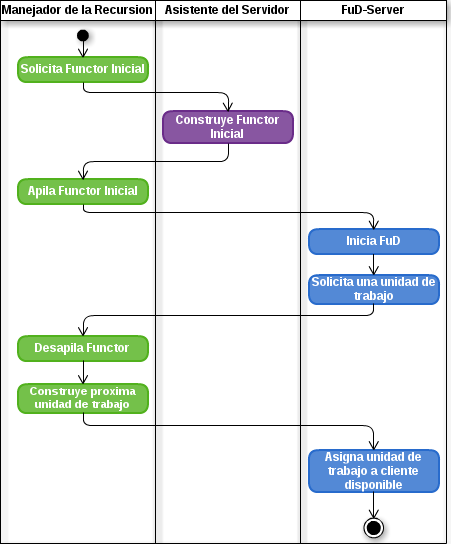
\includegraphics[scale=0.75]{images/ActivityRecAbs-1.png}
            \end{center}
            \caption{Diagrama de Actividades de inicio en servidor}
            \label{activity1}
        \end{figure}

    \subsubsection{Procesamiento en Cliente}
    En \ref{activity2} se ilustra mediante un diagrama de actividad el hilo de ejecución de un functor que llega a un
    cliente hasta su realización total, teniendo en cuenta también los casos en los que el cliente desee enviar
    resultados o mensajes en medio del proceso.

        \begin{figure}[!ht]
            \begin{center}

            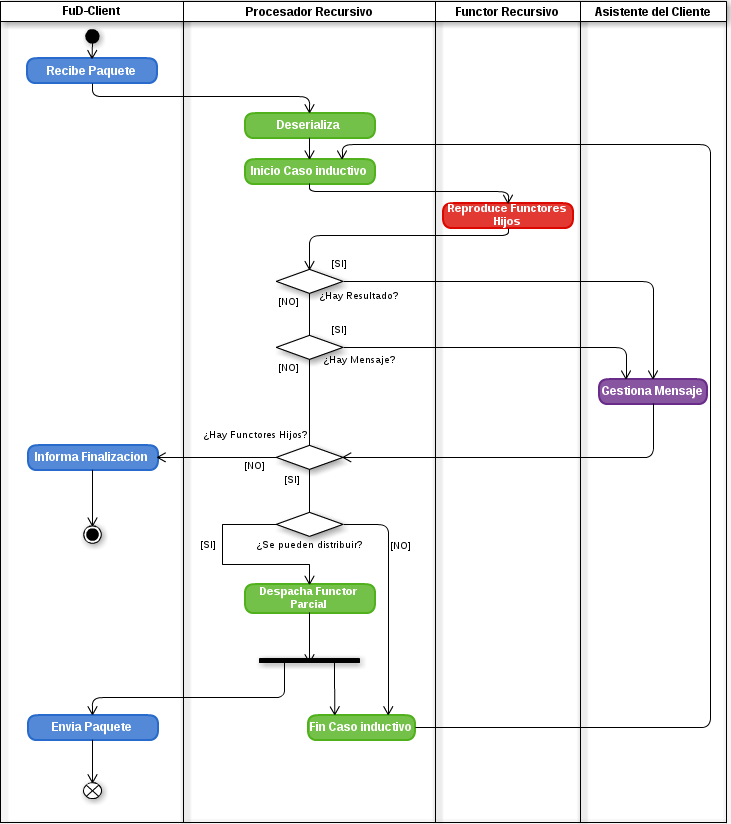
\includegraphics[scale=0.55]{images/ActivityRecAbs-2.png}
            \end{center}
            \caption{Diagrama de Actividades del procesamiento en Cliente}
            \label{activity2}
        \end{figure}


     \subsubsection{Recepción mensajes}
        Cada vez que \fud{} reciba un paquete, \rc{} analizará su tipo y tratará según corresponda. En caso de que
        lo arribado sea un mensaje o un resultado es el asistente quién se hará cargo, pero en cambio si lo que llega
        es otro functor recursivo resuelto parcialmente se apilará nuevamente para una futura distribución. 

            \begin{figure}[!ht]
                \begin{center}
                    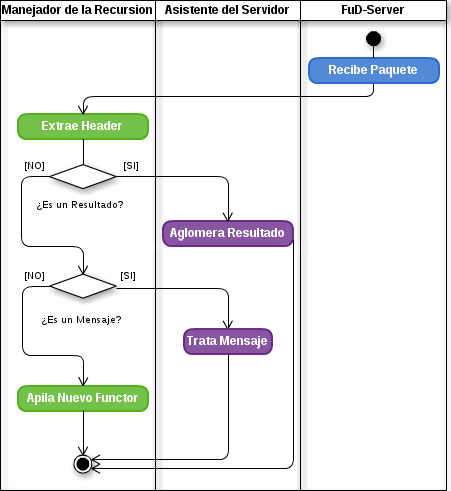
\includegraphics[scale=0.8]{images/ActivityRecAbs-3.png}
                    \end{center}
                    \caption{Diagrama de Actividades de recepción de mensajes}
                \label{activity3}
            \end{figure}

    \subsection{Aplicación}
        Para unificar todos los conceptos anteriores, la aplicación concreta deberá, en lado servidor, instanciar un
        Manejador de Recursión concreto, arrancarlo y luego informar los resultados. Por su parte, en el lado cliente,
        se deberá construir un procesador de recursión concreto e iniciarlo. Para mas detalles de como implementar y
        montar una aplicación concreta sobre \rc{} véase el capítulo \ref{chap:dummy_application}.


\section{Dependencias Externas}

Además de las bibliotecas STL (Standard Template Library) de cpp, recabs depende de otras bibliotecas, que se enuncian a continuación.

\subsection{MiLi}
\label{mili}

MiLi es una colección de pequeñas bibliotecas C++, compuesta únicamente por \textit{headers}. Sin necesidad de instalación, sin un
\textit{makefile}, sin complicaciones. Soluciones simples para problemas sencillos.

Esta biblioteca provee varias funcionalidades pequeñas en archivos cabecera (más conocidos como \textit{header files} en el ámbito de C/C++,
extensión ``.h'' o ``.hpp''), y puede ser descargada junto con su documentación en:
\begin{center}
    \texttt{http://mili.googlecode.com/}
\end{center}

MiLi ha sido utilizada extensamente a lo largo del desarrollo de  donde particularmente se destacan las funcionalidades provistas por
\textit{binary-streams} y \textit{container-utils}.

\begin{itemize}
    \item   \textbf{binary-streams:} esta biblioteca provee soporte a streams manejando información de cualquier tipo de objeto similar a
            como lo hace la biblioteca de entrada/salida estándar. En la Tabla \ref{bstreamuse} se muestra un ejemplo de su uso.
    \item   \textbf{container-utils:} esta biblioteca provee un conjunto de funciones, optimizadas para cada tipo de contenedor STL.
\end{itemize}

\begin{table}[!ht]
    \lstset{language=C++}
    \begin{lstlisting}[frame=single]
#include <iostream>
#include <string>
#include <vector>
#include "include/mili.h"

int main()
{
    std::vector<int> v(5,3); //all 3's
    v[1] = 1;
    v[4] = 7; //so it is [3,1,3,3,7]

    bostream bos;
    bos << 1 << 2 << 3 << std::string("Hello ") << v << 4 << std::string("World!");

    bistream bis(bos.str());

    int         nums[4];
    std::string str1;
    std::string str2;

    std::vector<int> v2;


    bis >> nums[0] >> nums[1] >> nums[2] >> str1 >> v2 >> nums[3] >> str2;

    for (int i=0; i < 4 ; ++i)
        std::cout << nums[i] << std::endl;

    std::cout << str1 << str2 << std::endl;

    std::cout << '[';
    for (size_t i=0; i < 5; ++i)
        std::cout<< v2[i] << ' ';
    std::cout << ']' << std::endl;
}
    \end{lstlisting}
    \centering \caption{C\'odigo extra\'ido de Mili::binary\_streams.}
    \label{bstreamuse}
\end{table}

\begin{table}[!htb]
    \lstset{language=C++}
    \begin{lstlisting}[frame=single]
#include <iostream>
#include <vector>
#include <string>
#include <queue>
#include "mili/mili.h"
using namespace std;

template <class T>
static void insert_elements(T& container);

int main()
{
    vector<int> v;
    v.push_back(1);
    map<string, string> m;
    m["hello"] = "good bye";
    m["Bonjour"] = "au revoir";
    m["hola"] = "adios";
    m["buenas"] = "adios";

    try
    {
        cout << contains(v, 2) << endl;         // will print 0 (false)
        cout << contains(m, "nothing") << endl; // will print 0

        cout << "map: " << endl;
        cout << remove_first_from(m, "au revoir") << endl; // will print 1
        cout << remove_all_from(m, "adios") << endl;       // will print 1

        cout << find(v, 1) << endl;         // will print 1 (true)
        cout << find(m, "hello") << endl;   // will print "good bye"
        cout << find(m, "world") << endl;   // will throw ElementNotFound
    }
    catch (ElementNotFound)
    {
        cerr << "Element not found!" << endl;
    }

    /* TEST - queue in container_utils::insert_into */
    queue<int> myqueue;
    insert_elements(myqueue);

    return 0;
}

template <class T>
static void insert_elements(T& container)
{
    insert_into(container, 100);
    insert_into(container, 100);
    insert_into(container, 100);
    insert_into(container, 200);
    insert_into(container, 300);
    insert_into(container, 400);
    insert_into(container, 400);
}
    \end{lstlisting}
    \centering \caption{C\'odigo extra\'ido de Mili::container\_utils.}
\end{table}

    \chapter{Diseño de \rc}

% Software Design
\textit{Diseñar} es el proceso de planificar y resolver problemas de un software en particular. Una vez que el propósito y las
especificaciones del software están determinados, debemos desarrollar un plan para llegar a una solución. Para llevarlo a cabo se incluyen
tanto la especificación de los diferentes módulos (o componentes) bien detallados, lo que llamamos \textbf{diseño de bajo nivel}, así como
el punto de vista arquitectónico o estructural, conocido como \textbf{diseño de alto nivel}.

\section{Diseño de Alto Nivel}

Desde el punto de vista de la ingeniería de software, el diseño de software es una etapa crucial del desarrollo de software, en la cual sus
implicaciones y deficiencias afectan el proyecto a lo largo de su ciclo de vida \cite{pressman}, por lo que la toma de decisiones sobre el
diseño es una tarea que debe ser llevada a cabo con especial atención y cuidado.

En esta tesis se emplearon \textit{principios de diseño de software}, los cuales representan un conjunto de directrices que nos ayudan a
evitar tener un mal diseño. Los principios de diseño se asocian a \textit{Robert Martin}, quien los reunió en el libro \textit{``Agile
Software Development: Principles, Patterns, and Practices''} \cite{martin-asd}. Según el autor, hay tres características importantes de un
mal diseño que deben evitarse:
\begin{itemize}
    \item   \textbf{Rigidez}: es difícil modificar porque cada cambio afecta a muchas otras partes del sistema.
    \item   \textbf{Fragilidad}: cuando hacemos un cambio, partes inesperadas del sistema se rompen.
    \item   \textbf{Inmovilidad}: es difícil reutilizar componentes en otra aplicación, ya que no se pueden desligar de la aplicación
            actual.
\end{itemize}
        
Para evitar estas \textit{malas} características, se intentó que el diseño cumpliese los principios fundamentales del diseño de software,
comúnmente conocidos por el acrónimo ``\textbf{SOLID}''\cite{objmentor} (\textbf{S}ingle responsibility, \textbf{O}pen-closed,
\textbf{L}iskov substitution, \textbf{I}nterface segregation y \textbf{D}ependency inversion). Aplicando estos principios de manera
conjunta, hacen más probable que un programador construya un sistema fácil de mantener y extensible en el tiempo.
\begin{description}
    \item   \textbf{Single Responsibility Principle (SRP)}: No debe existir más de una razón para que una clase cambie. Esto significa
            que una clase con diferentes responsabilidades debe ser dividida en clases más simples.
    \item   \textbf{Open-Closed Principle (OCP)}: Este principio establece que las entidades de software (clases, módulos, funciones,
            etc.) deben estar abiertas para su extensión pero cerradas para su modificación\cite{oosc}.
    \item   \textbf{Liskov Substitution Principle (LSP)}: Aquellas funciones que usan punteros o referencias a clases base deben ser capaces
            de utilizar objetos de clases derivadas, sin saberlo. Barbara Liskov lo describió unos 8 años antes \textit{Barbara Liskov} en
            el articulo \textit{``Data Abstraction and Hierarchy''} \cite{Liskov:1987:KAD:62139.62141} como:
            \begin{quote}
                \textit{Lo que se intenta aquí es algo como la siguiente propiedad de sustitución: Si para cada objeto o$_1$ de tipo S
                existe un objeto o$_2$ de tipo T tal que para todos los programas P definidos en t\'ermino de T, el comportamiento de P no
                se ve alterado cuando o$_1$ es sustituido por o$_2$, entonces S es un subtipo de T.}
            \end{quote}
    \item   \textbf{Interface Segregation Principle (ISP)}: Los clientes no deben ser forzados a depender de interfaces que no usan, lo que
            puede ser interpretado como el hecho de que las interfaces deben tener usuarios que las usen de manera completa, no parcial. Si
            este último fuese el caso, entonces debe haber otra interfaz con el subconjunto de métodos que este usuario particular
            necesita.
    \item   \textbf{Dependency Inversion Principle (DIP)}: Este principio establece dos puntos:
            \begin{itemize}
                \item   Módulos de alto nivel no deben depender de módulos de nivel más bajo. Ambos deben depender de abstracciones.
                \item   Abstracciones no deben depender de los detalles. Los detalles deben depender de las abstracciones.
            \end{itemize}   
\end{description}

Observando el diagrama OSI del framework \fud(\ref{sisd}) se puede observar claramente que el diseño se divide en dos partes, aplicaciones
cliente y servidor. A su vez, cada una de estas partes se encuentra organizada en 3 capas separadas, donde cada una de ellas posee una
responsabilidad bien definida.

%%%%%%%% ADD theories about client-server architecture. %%%%%%%%

Cabe destacar que el único enlace \textit{real} entre las aplicaciones cliente y servidor estará en el nivel más bajo, es decir, en
alguna implementación del \textit{middleware} de distribución (L1). Las restantes formas de comunicación son abstractas y deben
atravesar la estructura de capas.

\subsection{Arquitectura de \rc{} sobre \fud}

En la figura \ref{recabs_layers} se encuentra el diagrama al estilo OSI de redes donde se muestra una aplicación concreta, de solución
recursiva que es resulta usando \rc, el cual está montado sobre \fud. Este montaje respeta su arquitectura original (Véase
\ref{fud_layers}), agregando una nueva capa superior. En el mismo se muestran los componentes más importantes de este proyecto así como
también los mas relevantes del framework.

\begin{figure}[ht]
    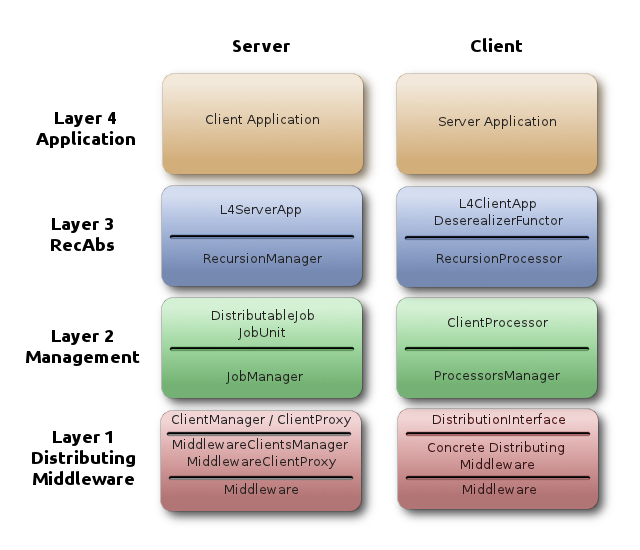
\includegraphics[scale=.6]{images/recabs.png}
    \caption{Capas de \texttt{RecAbs} + \texttt{FuD}}
    \label{recabs_layers}
\end{figure}

\subsection{Aplication Layer (L4)}

La ``capa aplicación'' proporciona los componentes que contienen todos los aspectos del dominio del problema en cuestión. Entre estos
aspectos se incluyen todas las definiciones de datos que se usan y la manipulación de los mismos, como así también, los algoritmos
relevantes para la solución del problema.

Es necesario aclarar que esta capa no forma parte de \rc(L3) ni del framework \fud(L2 y L1), así como cualquier código de aplicación que
usa una librería no forma parte de la misma. La inclusión de esta capa al diseño tiene como propósito la comprensión de cómo una aplicación
utiliza la biblioteca y, por lo tanto, el funcionamiento de la misma.

Para mantener la arquitectura cliente-servidor, esta capa se separa en lado cliente, lado servidor y también una parte común a ambos lados:
\begin{itemize}
    \item   \textbf{Lado Servidor}.\\
            Es necesario proveer a la capa subyacente el \textit{functor recursivo} inicial de la aplicación, y ademas, definir que hacer  
            con los mensajes intermedios y resultados que van llegando al servidor. Ver \ref{server_helper}.
    \item   \textbf{Lado Cliente}.\\
            Se necesitan proveer estos requerimientos:
            \begin{itemize}
                \item   la deserialización de un \textit{functor recursivo} a partir de los paquetes enviados de servidor a clientes. Para
                        ello, se cuenta se cuenta con MiLi, particularmente los \textit{binary streams}, que son de gran utilidad en
                        \textit{serialización} y \textit{deserialización} de paquetes.
                \item   la cantidad y el tiempo en que se envían mensajes o resultados desde el cliente hacia el servidor. Para ello se
                        cuenta con un interfaz e implementaciones concretas o bien, permite la propia que el usuario desee implementar (ver
                        \ref{client_helper}).
                \item   opcionalmente, se puede especificar una política de distribución propia, la cual establece cuándo y cuántas unidades
                        de trabajo se deben distribuir, dependiendo del estado en que se encuentre el servidor. Para más detalles vea
                        \ref{distribution_policy}.
            \end{itemize}
    \item   \textbf{Parte común}.\\
            Se debe proveer, a la capa L3, la definición de un \textit{functor recursivo} específico al problema que L4 desee atacar, por lo
            que básicamente se deben declarar cuáles son sus atributos necesarios y la serialización del mismo. Como se menciono en         
            \ref{functor}, un \textit{functor} representa a la función que el creador de la aplicación L4 desea distribuir a sus clientes
            para el posterior procesamiento en cada uno de ellos.
\end{itemize}


\subsection{\rc{} Layer (L3)}

Esta es la capa que provee el ``molde'' para definir soluciones a problemas que requieren un modelo recursivo (sin dependencias
horizontales dentro del árbol de recursión, ver \ref{problem_desc}) y, al mismo tiempo, provee una solución algorítmicamente
eficiente para dichos proyectos.

Siguiendo el mismo esquema de separación según la arquitectura cliente-servidor, las principales responsabilidades de esta capa son:
\begin{itemize}
    \item   \textbf{Lado Servidor}.\\
            La responsabilidad de esta capa es iniciar y administrar la recursión que haya propuesto la aplicación L4, y más
            específicamente, el servidor es el encargado de mantener una \textit{pila} de functores (nodos del árbol de recursión) que
            representa a los nodos que no han sido procesados todavía. De esta manera la capa subyacente solo deberá \textit{apilar} cuando
            llegue un nuevo nodo para procesar o \textit{desapilar} cuando se quiera obtener el próximo nodo para enviar a un cliente
            ocioso.

            Otra responsabilidad que toma el server es la de notificar a la capa superior de la llegada de mensajes y resultados, dejando
            el tratamiento de éstos como métodos a implementar.

            El servidor es el que inicia la recursión con el \textit{functor} inicial que es creado por la aplicación (L4).
    \item   \textbf{Lado Cliente}.\\
            El cliente es el encargado de realizar la ejecución total (o parcial) del functor que le fue asignado. Para cumplir su función
            se suple de las siguientes funcionalidades:
            \begin{itemize}
                \item   Deserialización de functores.
                \item   Descomposición del problema en más functores, de los cuales, si es posible, serán redistribuidos para repartir el
                        trabajo en varios clientes. Este paso comúnmente se apoya en un middleware de distribución HPC (en nuestro caso
                        \fud).
                \item   Política de distribución de functores, el cuál nos dirá cuándo y cuánto trabajo debemos
                        distribuir para que otros
                        clientes trabajen, y de esta forma balancear la carga de trabajo para cada cliente.
                \item   Envío de resultados o mensajes según la política que se use: enviar cada un determinado tiempo, cada tantos
                        bytes de memoria, etc.
            \end{itemize}

            Todo esta maquinaria hace que \textit{un} cliente procese sus resultados sin sobrecargar demasiado al servidor, permitiendo     
            distribuir functores que no estén siendo atendidos por él a clientes ociosos.
    \item   \textbf{Parte común}.\\
            Tanto el servidor como los clientes tienen la noción de estado de un \textbf{\textit{functor}}, el cual representa el estado
            particular de una función recursiva, y su función primordial es la de auto-reproducirse: genera una lista de sus functores
            hijos. Cuando se desee utilizar algún middleware de distribución, se manipula un tipo especial de \textit{functor}, el cuál
            además de las funciones mencionadas anteriormente, se le agrega la capacidad de serializarse, lo que permite una representación
            homogénea que todo cliente pueda deserializar llegado el momento de hacerlo.
\end{itemize}

\subsection{Diagrama de clases de \rc}

Para tener una visión macroscópica sobre el diseño de alto nivel, en la figura \ref{class_diagram} se presenta el \textit{diagrama de
clases} de \rc, el cuál netamente es sólo la capa de abstracción para soluciones recursivas (L3), acompañado de sus capas inmediatas: por un
lado está la capa subyacente (L2) que simboliza la parte alta del framework de distribución \fud, y por otro lado la capa superior (L4) la
cuál representa una aplicación que usa la librería \rc.

\begin{center}
    \begin{landscape}
        \begin{figure}[ht]
            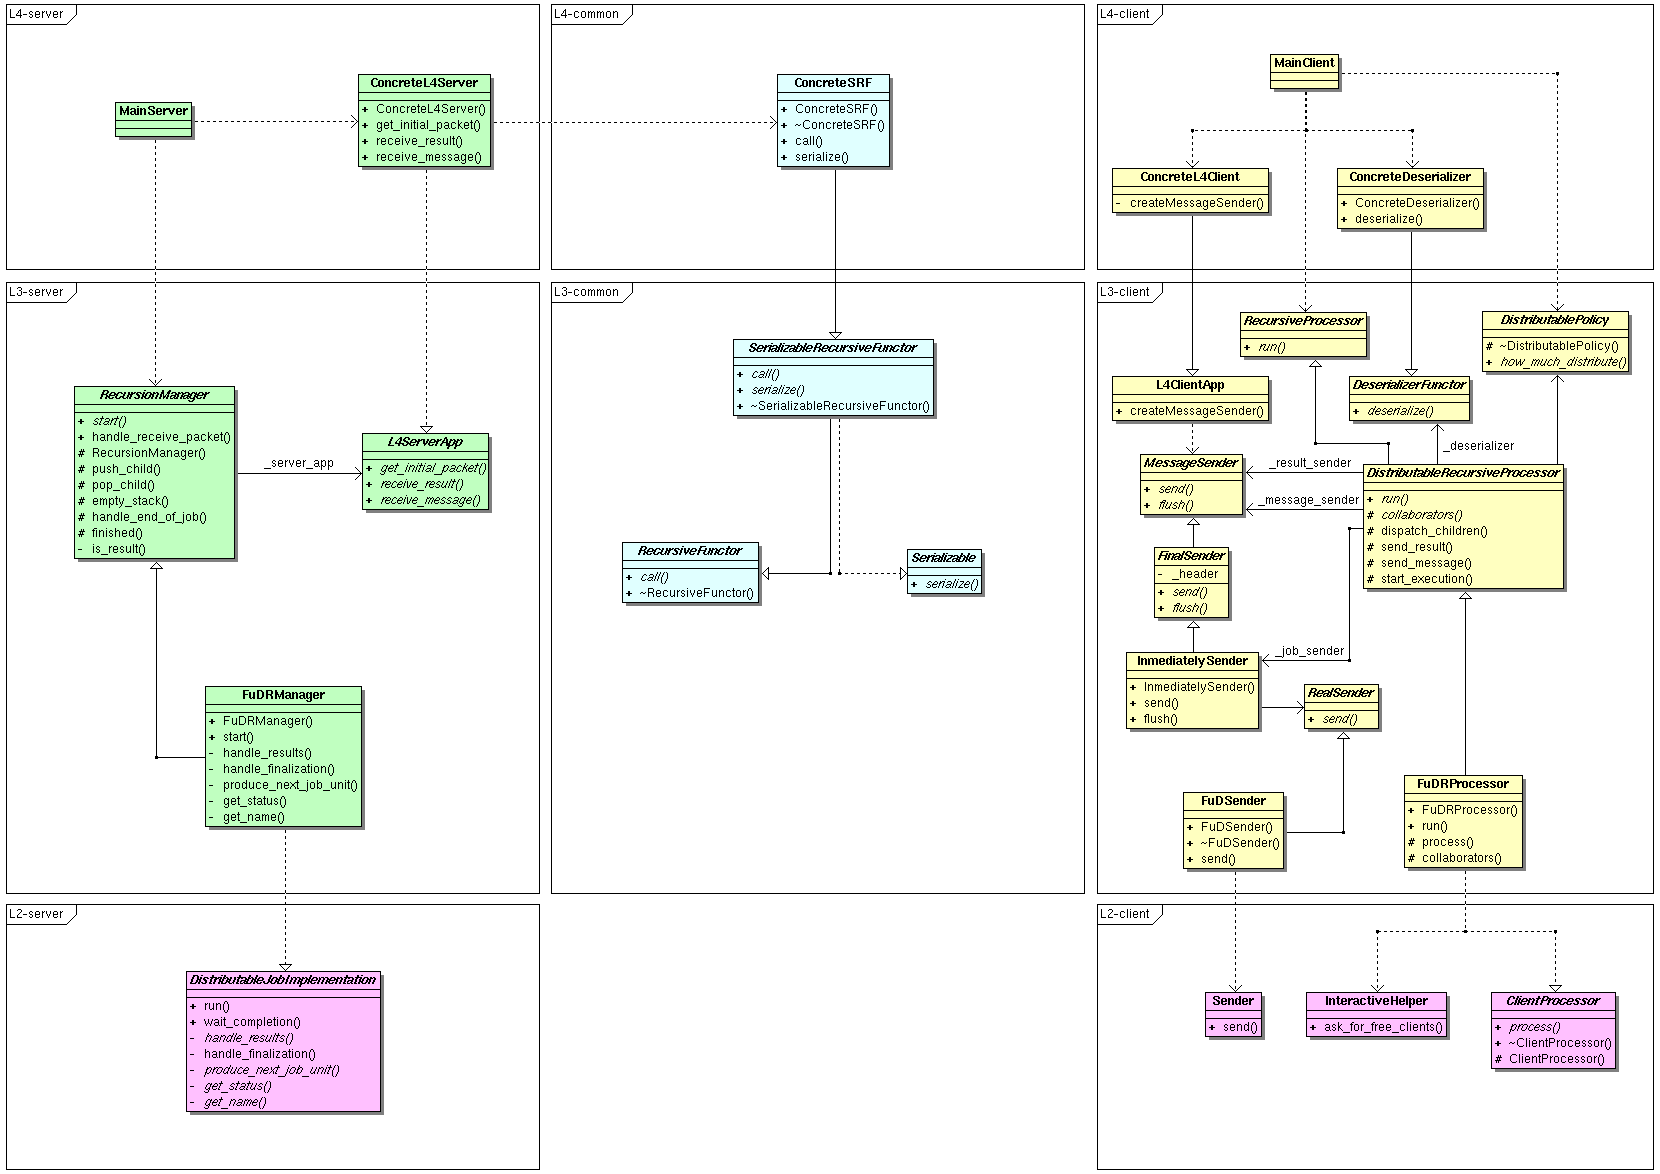
\includegraphics[scale=.35]{images/class.png}
            \caption{Diagrama de clases de \rc \ y sus capas inmediatas}
            \label{class_diagram}
        \end{figure}
    \end{landscape}
\end{center}


\section{Diseño de Bajo Nivel}

Aquí se hace un refinamiento de las decisiones de diseño sobre aquellos componentes abstractos presentes en el
diseño de alto nivel. Además, se analiza cómo estas clases están compuestas: los atributos de cada una, los métodos que
declaran y sus interacciones con el resto del sistema. 

A continuación se describen los módulos mas importantes de la capa \rc{}, detallando las decisiones tenidas en
cuenta a la hora de diseñarlos. Para cada componente del módulo se muestra un diagrama de clases
simplificado.

\subsection{Functor Recursivo}

Anteriormente se describió abstractamente el concepto de un Functor Recursivo. Con el fin
de modelar este concepto se estableció esta jerarquía de clases:
    
    \subsubsection{\texttt{RecursiveFunctor}}
        Todo functor es representado por una implementación de la interfaz \\ \texttt{RecursiveFunctor} que publica el
        método \texttt{call}. Por tanto, una aplicacion concreta deberá implementar este método dando creación a un
        nuevo \textit{functor} que representará la función que el usuario desee distribuir.

        \begin{figure}[ht] \hspace{4.5cm}
            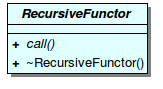
\includegraphics[scale=.75]{images/rf.png}
            \caption{Clase \texttt{RecursiveFunctor}}
        \end{figure}
        
    \begin{itemize}
        \item \texttt{call(ChildrenFunctors\& children, Packet\& result, WhenToSend\& when)}
               Este método deberá encapsular el comportamiento de la función recursiva a modelar de manera que se
               especifiquen el contenido de los parámetros de la siguiente forma:
        \begin{description}
            \item[children] Rellenar con los functores resultantes de un paso de la recursión del proceso.
            \item[result]   Aquí va un mensaje hacia el servidor, puede ser de dos tipos según el momento del
                            procesamiento en el que se encuentre. En caso de estar en el final de un nodo, o sea en
                            el caso base, donde \texttt{children} será una lista vacía, el mensaje deberá contener el
                            resultado ya serializado. De esta manera \texttt{message} será enviado al servidor y
                            tratado como como un resultado final del nodo corriente. Pero en el caso de que el nodo este
                            en medio de una rama y se quiera enviar un mensaje a la aplicación lado servidor se
                            puede usar este parámetro para notificar mediante un mensaje serializado, por ejemplo,
                            el estado actual el procesamiento.
            \item[when] Mediante un tipo enumerado, especificar el momento del envío del mensaje o resultado. Esto
                        puede ser \texttt{kSendThisImmediately}, el cual indica que el mensaje sea enviado
                        inmediatamente; \\ \texttt{kSendAllImmediately} indica que el mensaje sea enviado inmediatamente
                        junto con el resto de los mensajes en espera y por ultimo \texttt{kSendWhenRecAbsWants} donde se
                        le otorga a \rc{} la responsabilidad de enviarlo cuando éste lo disponga.
        \end{description}
    \end{itemize}

    \subsubsection{\texttt{SerializableRecursiveFunctor}}

        Es la versión serializable de la clase descrita anteriormente, es decir hereda directamente de
        \texttt{RecursiveFunctor} agregando un método extra también puro virtual para proporcionar la
        funcionalidad de serialización y permitir el envío de estos functores a través de algún middleware de
        distribución.

        \begin{figure}[!htb] \hspace{3.8cm}
            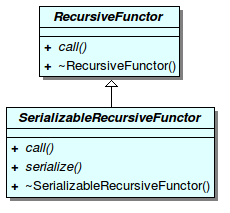
\includegraphics[scale=0.75]{images/srf.png}
            \caption{Clase \texttt{SerializableRecursiveFunctor}}
        \end{figure}
   
    \begin{itemize}
        \item \texttt{void serialize(Packet\& pkt)}

        Aquí un functor concreto deberá implementar la serialización, especificando de que manera el objeto es
        empaquetado en \texttt{pkt}
    \end{itemize}


\subsection{Asistente del Servidor}

Ya habíamos introducido en \ref{server_helper} las responsabilidades de este asistente. Se realizó una interfaz que
será implementada por el desarrollador de una aplicación, especificando métodos necesarios para iniciar la ejecución del
servidor y para asimilar los resultados arrojados.

\subsubsection{\texttt{L4ServerApp}}

Esta interfaz brindará el \textit{functor} inicial y definirá que se hará con los resultados y mensajes intermedios a medida que
lleguen. Ver clase en figura \ref{l4_server_app}.

\begin{figure}[ht] \hspace{4.8cm}
    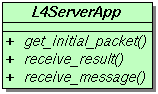
\includegraphics[scale=.68]{images/l4_server_app.png}
    \caption{Clase \texttt{L4ServerApp}.}
    \label{l4_server_app}
\end{figure}

\begin{itemize}
    \item \texttt{void get\_initial\_packet(Packet\& pkt)}\\[0.2cm]
                Deberá retornar (en el parámetro \texttt{pkt}) un paquete de datos que represente al \textit{functor} inicial de la
                aplicación. Debido a que este \textit{paquete} es la serialización de un \textit{functor}, las clases hijas tendrán una
                relación con el \texttt{RecursiveFunctor} del problema corriente. Dado el ejemplo de la figura
                \ref{l4_server_app_with_srf}, ver que una implementación concreta de \texttt{L4ServerApp} necesariamente deberá ``conocer''
                al \texttt{SerializableRecursiveFunctor} concreto para poder crear el \textit{functor} inicial y luego llamar al método
                \texttt{serialize()}, el cual lo retorna como un paquete. Dicho paquete inicial será enviado a un cliente, para que sea éste
                quién inicie la ejecución  de la aplicación.
    \item \texttt{void receive\_result(const Packet\& result)}\\[0.2cm]
                Durante el procesamiento de un \textit{functor}, los clientes pueden enviar resultados al servidor. Éste método es el que
                define que se harán con los mismos.
    \item \texttt{void receive\_message(const Packet\& msg)}\\[0.2cm]
                Durante el procesamiento de un \textit{functor}, los clientes pueden enviar mensajes intermedios al servidor. Éste método es
                el que define que se harán con los mismos. Cabe aclarar, que a diferencia de los resultados, éstos pueden ser enviados en
                cualquier momento de la etapa de recursión, y no, como los resultados, sólo en las hojas pertenecientes al árbol de
                recursión, generado por el \textit{functor} ejecutado.
\end{itemize}

\begin{figure}[ht] \hspace{1.8cm}
    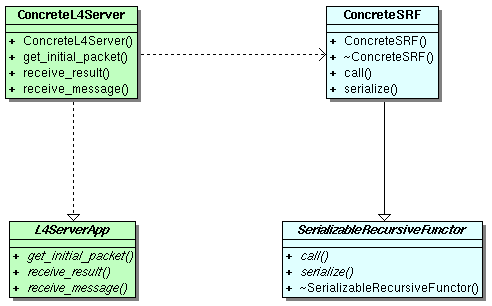
\includegraphics[scale=.6]{images/l4_server_app_with_srf.png}
    \caption{Colaboración \texttt{L4ServerApp} - \texttt{SerializableRecursiveFunctor}.}
    \label{l4_server_app_with_srf}
\end{figure}


\subsection{Administrador de recursión}
    Es quién organiza y manipula los functores pendientes del proceso recursivo, interactúa con el middleware de
distribución para tal propósito. Para más detalles de sus responsabilidades véase la sección \ref{rmanager}.

\subsubsection{\texttt{RecursionManager}}

Es la clase que modela un \textit{administrador de recursión}. En la figura \ref{recursion_manager} está graficada su entidad.

\begin{figure}[ht] \hspace{4.7cm}
    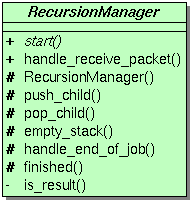
\includegraphics[scale=.6]{images/recursion_manager.png}
    \caption{Clase \texttt{RecursionManager}.}
    \label{recursion_manager}
\end{figure}

Las \textit{unidades de trabajo} se mantienen en una pila, la cual se va desapilando a medida que haya usuarios ociosos. Debido a ello, la
clase cuenta con un basto número de operaciones que manejan esta pila, y también posee métodos que conocen de la finalización de la
ejecución total de la aplicación y del cómputo de cada \textit{functor}.

\texttt{RecursionManager} tiene el método \texttt{start()} que deja como abstracto para las posibles implementaciones según el middleware
que se utilice en la capa subyacente. Este método deberá iniciar la ejecución total de cualquier proyecto que use la librería.

Para realizar su trabajo cuenta con la colaboración de la interfaz \texttt{L4ServerApp}, el cuál nos brinda el functor inicial, que es dado
al primer cliente dando así la iniciación del proceso recursivo, y es el procesador de resultados y mensajes de los clientes que computan
sus funciones.

\begin{figure}[ht] \hspace{1.5cm}
    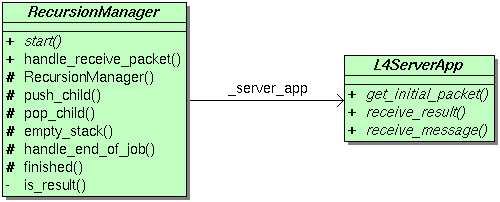
\includegraphics[scale=.6]{images/rec_manager_with_l4_server_app.png}
    \caption{Colaboración \texttt{RecursionManager} - \texttt{L4ServerApp}.}
    \label{rec_manager_with_l4_server_app}
\end{figure}


\subsubsection{\texttt{FuDRManager}}

Es el administrador de recursión específico del framework de distribución \fud. Como dijimos anteriormente, este implementa la rutina
\texttt{start()} y de esta forma es una realización concreta del administrador de recursión. Cabe aclarar que esta clase es un ``sabor'',
una posible implementación, no es la única, y cada concretización de un \textit{manager} dependerá del modelo de distribución que se quiera
utilizar en la capa inferior. Como resultado de este montaje, las aplicaciones correrán sobre el framework \fud{} implementando métodos de
\texttt{DistributableRecursiveProcessor}. Véase \ref{fud_manager_dji}.

\begin{figure}[ht] \hspace{4.5cm}
    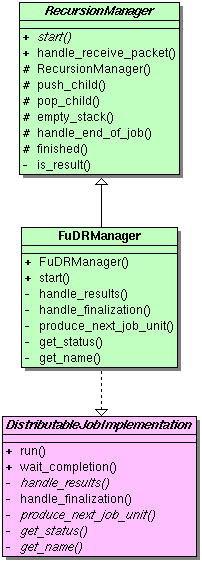
\includegraphics[scale=.6]{images/fud_manager_dji.png}
    \caption{Clase \texttt{FuDRManager}.}
    \label{fud_manager_dji}
\end{figure}


\subsection{Procesador Recursivo}

Este módulo representa el engine de ejecución recursiva, es decir, es el cerebro del procesamiento local en un
nodo de un functor recursivo. Fué diseñado con una jerarquía de \texttt{processors} donde cada uno va
adhiriendo responsabilidades con el fin de permitir otras implementaciones de este engine sin mucho costo de
acoplamiento.
    
    \subsubsection{\texttt{RecursiveProcessor}}

        Interfaz que representa el engine genérico publicando el método \texttt{run}, el cual deberá
        implementar todo procesador concreto. Ver \ref{rp}.

        \begin{figure}[ht] \hspace{4.8cm}
            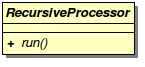
\includegraphics[scale=0.75]{images/rp.png}
            \caption{Clase \texttt{RecursiveProcessor}}
            \label{rp}
        \end{figure}
        
        \begin{itemize}
            \item \texttt{void run(const Address\& address = LOCALHOST, Port port = DEFAULT\_PORT)}
                Método responsable de iniciar el proceso en un nodo de procesamiento.
                \begin{description}
                \item[address] IP del servidor.
                \item[port] el puerto del servidor.
                \end{description}
        \end{itemize}

    \subsubsection{\texttt{DistributableRecursiveProcessor}}

        Es la versión \textit{distribuible} de
        \texttt{RecursiveProcessor}, agregando funcionalidad de interacción con el servidor de modo que pueda consultar
        sobre disponibilidad, enviar trabajos incompletos, enviar mensajes o resultados al servidor.
        Ésta clase también engloba a toda implementación de un procesador que necesite distribución de trabajos, por
        tanto si bien provee toda la maquinaria para lograr la distribución, deja libre a cualquier plataforma de
        comunicación la implementación del middleware, por tanto delega la definición del método \texttt{run}. (Véase
        \href{DistributableRecursiveProcessor})

        \begin{figure}[ht] \hspace{3.8cm}
            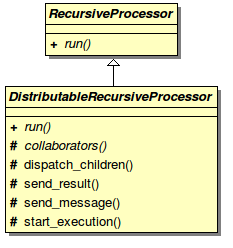
\includegraphics[scale=0.75]{images/drp.png}
            \caption{Clase \texttt{DistributableRecursiveProcessor}}
            \label{DistributableRecursiveProcessor} 
        \end{figure}

%         \begin{itemize}
%             \item \footnotesize{\texttt{virtual void start\_execution(const Packet\& init\_packet))}}\\
% 
%             \item \footnotesize{\texttt{void do\_recursion(ChildrenFunctors\& functor\_list)}}
% 
%             \item \footnotesize{\texttt{void reproduce(RecursiveFunctor* rf, ChildrenFunctors\& functor\_list)}}
% 
%             \item \footnotesize{\texttt{void send\_result(const Packet\& packet, WhenToSend when)}}
% 
%             \item \footnotesize{\texttt{void send\_message(const Packet\& packet, WhenToSend when)}}
%         \end{itemize}

        
    \subsubsection{\texttt{FuDRProcessor}}

        Es el procesador recursivo distribuible concreto que en parte monta al cliente \rc{} sobre el cliente \fud{}.
        Implementa el método \texttt{run} de \\ \texttt{DistributableRecursiveProcessor} el cual será invocado una sola
        vez al comienzo del procesamiento nodal. Es una pieza fundamental en el montaje con \fud{} ya que describe a
        \rc{} como una aplicación que correrá sobre el framework implementando métodos de \texttt{ClientProcessor}.
        (Véase \ref{FuDRProcessor})
    
        \begin{figure}[ht] \hspace{4.2cm}
            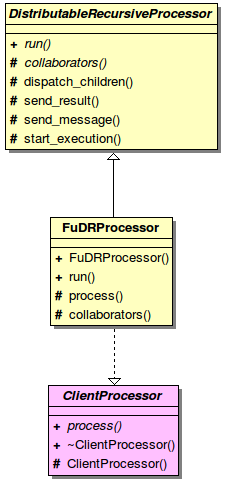
\includegraphics[scale=0.70]{images/frp.png}
            \caption{Clase \texttt{FuDRProcessor}}
             \label{FuDRProcessor}
        \end{figure}


\subsection{Deserializador}

Cuando un functor arriba a un cliente, éste se encuentra codificado para que el servidor pudiese enviarlo.
Es responsabilidad de este módulo de especificar de que manera se realiza el método inverso a la serialización
realizada en el lado servidor. Por cada functor concreto se tendrá que implementar esta deserialización.

    \subsubsection{\texttt{DeserializerFunctor}}
        Interface que publica el método puro virtual \texttt{deserialize}

        \begin{figure}[!htb] \hspace{4.8cm}
            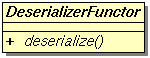
\includegraphics[scale=0.70]{images/deserializer.png}
            \caption{Clase \texttt{DeserializerFunctor}}
             \label{Deserializer}
        \end{figure}

        \begin{itemize}
            \item \texttt{deserialize(const Packet\& p, SerializableRecursiveFunctor** rf)}

                Método que será invocado por \texttt{DistributableRecursionProcessor} al incio del procesamiento local.
                \begin{description}
                \item[p]: Es el functor enviado por el server ya serializado.
                \item[rf]: Aquí se deberá dejar el functor ya deserializado.
                \end{description}
        \end{itemize}
    
    
\subsection{Senders}

    Aquí se define la lógica de tratamiento de mensajes (tanto mensajes propiamente dichos como resultados) antes de
ser enviados al servidor. Lo cual implica definir con que middleware de distribución se harán los envíos así como
también los diferentes criterios de manipulación. Para lograr esto se usó el patrón \textit{Chain of Responsibility}
(\textit{Véase} \ref{chain_pattern}) ya que se brinda al usuario final la posibilidad de encadenar distintos senders
ficticios que irán realizando alguna tarea particular con los mensajes a enviar, como por ejemplo, la acumulación de los
mismos a efectos de no congestionar la red y enviar un solo paquete con muchos mensajes dentro.

    \subsubsection{\texttt{MessageSender}}
        Este es el concepto genérico de un sender, una clase abstracta que define dos métodos

        \begin{figure}[!htb] \hspace{5.2cm}
            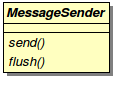
\includegraphics[scale=0.70]{images/sender.png}
            \caption{Clase \texttt{MessageSender}}
             \label{MessageSender}
        \end{figure}

        \begin{itemize}
            \item \texttt{void send(const PacketContainer\& packet\_container) = 0;}\\
                Manipula el mensaje según algún criterio para un posterior envío, o bien efectúa el envío del mensaje al
                server en el acto.
                \begin{description}
                    \item[packet\_container]: Colección de mensajes a enviar.
                \end{description}

            \item \texttt{void flush()}\\
                Fuerza el envío de mensaje en el instante que se invoca.
        \end{itemize}

    \subsubsection{\texttt{FinalSender \& ChainableSender}}

        Existen dos \textit{familias} de senders:
        \begin{itemize}
            \item \textbf{Finales:} aquellos que hacen efectivo el envío mediante una colaboración con el
                 middleware. Se implementó un sender final concreto que se llama \texttt{InmediatelySender} el
cuál envía el mensaje en el momento. Este tiene una relación con la clase \texttt{RealSender} quien se encarga
efectivamente del envío \textit{real} al servidor.
            \item \textbf{Encadenables:} no son senders finales, desconocen el middleware subyacente, por eso el
método \texttt{send} no necesariamente realiza el envío real al servidor. Estos senders pueden manipular los mensajes
con algún fin en particular antes de enviárselo al servidor.

Tienen la particularidad de que se pueden encadenar, haciendo
que cada uno luego de realizar la acción deseada le pase el mensaje al sender siguiente para que éste realice su propia
acción y así sucesivamente. Por lo tanto es decisión de cada \texttt{ChainableSender} cuando entregarle el mensaje a su
sender mas próximo. Siempre en el final de esta cadena se encontrará algun \texttt{FinalSender} concreto que hará
efectivo el envío.


     Aquí el método flush forzará pasar el mensaje al próximo sender, el cual hará lo mismo con el que sigue, llegando
en algún momento a un \texttt{FinalSender} y efectuar el envío del mensaje en el estado que se encuentre.


Un \texttt{ChainableSender} puede realizar tareas de acumulación, compresión, encriptación, etc. En el contexto de este
proyecto se realizo la implementación de un sender que acumula mensajes hasta una cantidad de $N$ bytes fijos
(\texttt{BySizeResultSender}).
                
        \end{itemize}
            \begin{figure}[!htb] \hspace{0cm}
            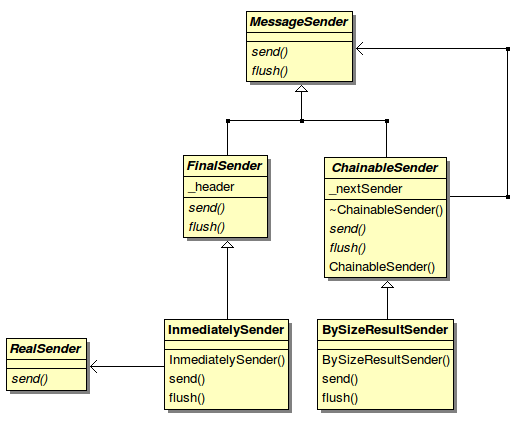
\includegraphics[scale=0.70]{images/senders.png}
            \caption{Colaboración entre los distintos \texttt{senders}}
            \label{MessageSenders}
        \end{figure}


\subsection{Asistente del cliente}

Es uno de los componentes que el usuario final podrá extender, en este caso para decirle a capa subyacente detalles de
como enviar mensajes al servidor. \rc{} al comienzo del proceso solicita al asistente del cliente el
\texttt{MessageSender} de la aplicación, por tanto se debe redefinir el método \\ \texttt{createMessageSender} con la
cadena de senders deseada o bien, dejar el asistente por defecto que encadena un sender de acumulación por bytes con
uno real.

        \begin{figure}[!htb] \hspace{2cm}
            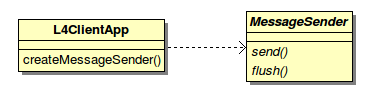
\includegraphics[scale=0.70]{images/l4_client_app.png}
            \caption{Colaboración \texttt{L4ClientApp} - \texttt{MessageSender}}
            \label{l4ca_sender}
        \end{figure}

\subsection{Política de Distribución}

Hicimos una breve introducción de este tema en \ref{distribution_policy}. Las políticas definen cuándo un cliente debe distribuir sus
unidades de trabajo pendientes o cuándo no debe y, en caso positivo, cuánto debe distribuir. El propósito de este módulo es
\textit{balancear la carga} (\textit{load balancing}, en inglés), técnica usada para compartir el trabajo a realizar entre varios recursos,
la cuál es lograda gracias a un algoritmo que divide de la manera más equitativa posible el trabajo.

% Performance
Este tipo de políticas puede influenciar mucho en la performance de una aplicación ya que el costo de comunicación en la distribución de
paquetes entre el servidor y sus clientes varía en poca o gran medida dependiendo principalmente de:
\begin{itemize}
    \item   el nivel de procesamiento que requiera la aplicación concreta en cuestión, y
    \item   de los recursos con que se cuenten (tanto en servidor como en clientes).
\end{itemize}

\subsubsection{\texttt{DistributablePolicy}}

Clase abstracta que representa cualquier política de distribución, dejando el método \texttt{how\_much\_distribute} puro virtual, el cuál
deberá ser implementado por todo usuario de la librería que desee una política ``a su gusto''.

\rc{} tiene incluido por defecto diferentes políticas de distribución, con el propósito de mostrar ``implementaciones de juguete'' y, en el
caso de la \texttt{Sigmoid}, para tener una buena política como punto de partida, la cuál fue usada en la aplicación que se dará como
ejemplo en un capítulo siguiente. En la figura \ref{distribution_policy_class} se encuentran estas políticas pre
establecidas, de las cuáles sólo
explicaremos a continuación las más relevantes.

\begin{figure}[hb]
    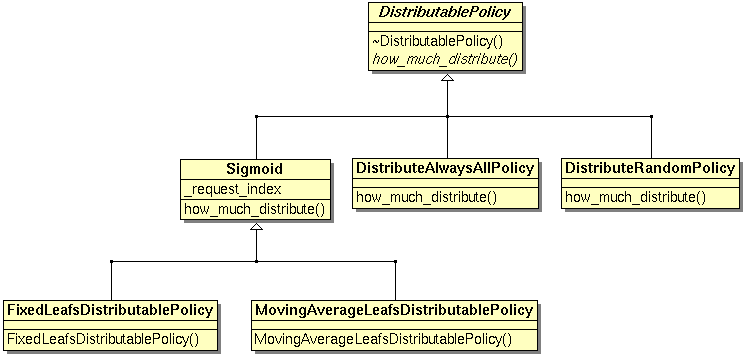
\includegraphics[scale=.6]{images/distribution_policy.png}
    \caption{Diagrama de políticas de distribución.}
    \label{distribution_policy_class}
\end{figure}

\subsubsection{\texttt{DistributeAllwaysAllPolicy}}

Está es una implementación trivial de política de distribución, y consiste en enviar siempre el máximo de unidades de trabajo que se
pueda enviar.

\subsubsection{\texttt{Sigmoid}}

Esta política describe una \textit{función sigmoidea decreciente} teniendo en cuenta el \textbf{nivel de profundidad} (en el árbol de
recursión generado por la ejecución) en el cual el functor está siendo ejecutado, ademas de las constantes: \textit{cantidad de hijos},
\textit{hojas finales} e \textit{índice de ajuste}. La fórmula que se utilizó para describir esta política es la siguiente:

\begin{center}
    \Large{$fsd(x) = \frac{children-1}{1 + e^{-(\log_{children}{leafs}) * index + x - (children-1)}} $}
\end{center}
donde:
\begin{itemize}
    \item   $children$: \textit{cantidad de hijos} que genera un functor en \textit{un} sólo paso.
    \item   $leafs$: cantidad de \textit{hojas finales} (o casos bases) que generará el cálculo completo de la aplicación corriente.
    \item   $index$: \textit{índice de ajuste}, valores altos significan más consultas al servidor sobre disponibilidad de clientes libres
            y, en contraposición, valores bajos corresponden a una mayor autosuficiencia en la ejecución de functores propios a un cliente.
\end{itemize}

El resultado de está función nos arrojará cuantos \textit{functores} podemos distribuir en relación al nivel de profundidad de manera tal
que a medida que un cliente procesa un functor con niveles cada vez más altos, el cliente distribuye menos functores y procesa más por su
cuenta. El propósito de está función es no sobrecargar al servidor de consultas sobre disponibilidad de clientes libres y la de tener un
punto (o nivel) en el cuál cada cliente sea autosuficiente en cuanto a procesamiento.

A modo de ejemplo, la figura \ref{fsi} muestra una función específica fijando la \textit{cantidad de hijos} en $8$, la cantidad de
\textit{hojas finales} en $1000$ y el \textit{índice de ajuste} en $0.5$.

\begin{figure}
    % GNUPLOT: LaTeX picture
    \setlength{\unitlength}{0.240900pt}
    \ifx\plotpoint\undefined\newsavebox{\plotpoint}\fi
    \begin{picture}(1500,900)(0,0)
    \sbox{\plotpoint}{\rule[-0.200pt]{0.400pt}{0.400pt}}%
    \put(131.0,131.0){\rule[-0.200pt]{4.818pt}{0.400pt}}
    \put(111,131){\makebox(0,0)[r]{ 0}}
    \put(1419.0,131.0){\rule[-0.200pt]{4.818pt}{0.400pt}}
    \put(131.0,228.0){\rule[-0.200pt]{4.818pt}{0.400pt}}
    \put(111,228){\makebox(0,0)[r]{ 1}}
    \put(1419.0,228.0){\rule[-0.200pt]{4.818pt}{0.400pt}}
    \put(131.0,325.0){\rule[-0.200pt]{4.818pt}{0.400pt}}
    \put(111,325){\makebox(0,0)[r]{ 2}}
    \put(1419.0,325.0){\rule[-0.200pt]{4.818pt}{0.400pt}}
    \put(131.0,422.0){\rule[-0.200pt]{4.818pt}{0.400pt}}
    \put(111,422){\makebox(0,0)[r]{ 3}}
    \put(1419.0,422.0){\rule[-0.200pt]{4.818pt}{0.400pt}}
    \put(131.0,519.0){\rule[-0.200pt]{4.818pt}{0.400pt}}
    \put(111,519){\makebox(0,0)[r]{ 4}}
    \put(1419.0,519.0){\rule[-0.200pt]{4.818pt}{0.400pt}}
    \put(131.0,616.0){\rule[-0.200pt]{4.818pt}{0.400pt}}
    \put(111,616){\makebox(0,0)[r]{ 5}}
    \put(1419.0,616.0){\rule[-0.200pt]{4.818pt}{0.400pt}}
    \put(131.0,713.0){\rule[-0.200pt]{4.818pt}{0.400pt}}
    \put(111,713){\makebox(0,0)[r]{ 6}}
    \put(1419.0,713.0){\rule[-0.200pt]{4.818pt}{0.400pt}}
    \put(131.0,810.0){\rule[-0.200pt]{4.818pt}{0.400pt}}
    \put(111,810){\makebox(0,0)[r]{ 7}}
    \put(1419.0,810.0){\rule[-0.200pt]{4.818pt}{0.400pt}}
    \put(131.0,131.0){\rule[-0.200pt]{0.400pt}{4.818pt}}
    \put(131,90){\makebox(0,0){ 0}}
    \put(131.0,839.0){\rule[-0.200pt]{0.400pt}{4.818pt}}
    \put(276.0,131.0){\rule[-0.200pt]{0.400pt}{4.818pt}}
    \put(276,90){\makebox(0,0){ 2}}
    \put(276.0,839.0){\rule[-0.200pt]{0.400pt}{4.818pt}}
    \put(422.0,131.0){\rule[-0.200pt]{0.400pt}{4.818pt}}
    \put(422,90){\makebox(0,0){ 4}}
    \put(422.0,839.0){\rule[-0.200pt]{0.400pt}{4.818pt}}
    \put(567.0,131.0){\rule[-0.200pt]{0.400pt}{4.818pt}}
    \put(567,90){\makebox(0,0){ 6}}
    \put(567.0,839.0){\rule[-0.200pt]{0.400pt}{4.818pt}}
    \put(712.0,131.0){\rule[-0.200pt]{0.400pt}{4.818pt}}
    \put(712,90){\makebox(0,0){ 8}}
    \put(712.0,839.0){\rule[-0.200pt]{0.400pt}{4.818pt}}
    \put(858.0,131.0){\rule[-0.200pt]{0.400pt}{4.818pt}}
    \put(858,90){\makebox(0,0){ 10}}
    \put(858.0,839.0){\rule[-0.200pt]{0.400pt}{4.818pt}}
    \put(1003.0,131.0){\rule[-0.200pt]{0.400pt}{4.818pt}}
    \put(1003,90){\makebox(0,0){ 12}}
    \put(1003.0,839.0){\rule[-0.200pt]{0.400pt}{4.818pt}}
    \put(1148.0,131.0){\rule[-0.200pt]{0.400pt}{4.818pt}}
    \put(1148,90){\makebox(0,0){ 14}}
    \put(1148.0,839.0){\rule[-0.200pt]{0.400pt}{4.818pt}}
    \put(1294.0,131.0){\rule[-0.200pt]{0.400pt}{4.818pt}}
    \put(1294,90){\makebox(0,0){ 16}}
    \put(1294.0,839.0){\rule[-0.200pt]{0.400pt}{4.818pt}}
    \put(1439.0,131.0){\rule[-0.200pt]{0.400pt}{4.818pt}}
    \put(1439,90){\makebox(0,0){ 18}}
    \put(1439.0,839.0){\rule[-0.200pt]{0.400pt}{4.818pt}}
    \put(131.0,131.0){\rule[-0.200pt]{0.400pt}{175.375pt}}
    \put(131.0,131.0){\rule[-0.200pt]{315.097pt}{0.400pt}}
    \put(1439.0,131.0){\rule[-0.200pt]{0.400pt}{175.375pt}}
    \put(131.0,859.0){\rule[-0.200pt]{315.097pt}{0.400pt}}
    \put(30,495){\makebox(0,0){f(x)}}
    \put(785,29){\makebox(0,0){x}}
    % \put(1279,819){\makebox(0,0)[r]{7 / (1 + exp(-((log(1000)/log(8)) * 0.5)+x-7))}}
    % \put(1299.0,819.0){\rule[-0.200pt]{24.090pt}{0.400pt}}
    \put(131,810){\usebox{\plotpoint}}
    \put(276,808.67){\rule{3.373pt}{0.400pt}}
    \multiput(276.00,809.17)(7.000,-1.000){2}{\rule{1.686pt}{0.400pt}}
    \put(131.0,810.0){\rule[-0.200pt]{34.930pt}{0.400pt}}
    \put(329,807.67){\rule{3.132pt}{0.400pt}}
    \multiput(329.00,808.17)(6.500,-1.000){2}{\rule{1.566pt}{0.400pt}}
    \put(290.0,809.0){\rule[-0.200pt]{9.395pt}{0.400pt}}
    \put(356,806.67){\rule{3.132pt}{0.400pt}}
    \multiput(356.00,807.17)(6.500,-1.000){2}{\rule{1.566pt}{0.400pt}}
    \put(342.0,808.0){\rule[-0.200pt]{3.373pt}{0.400pt}}
    \put(382,805.67){\rule{3.132pt}{0.400pt}}
    \multiput(382.00,806.17)(6.500,-1.000){2}{\rule{1.566pt}{0.400pt}}
    \put(395,804.67){\rule{3.132pt}{0.400pt}}
    \multiput(395.00,805.17)(6.500,-1.000){2}{\rule{1.566pt}{0.400pt}}
    \put(408,803.67){\rule{3.373pt}{0.400pt}}
    \multiput(408.00,804.17)(7.000,-1.000){2}{\rule{1.686pt}{0.400pt}}
    \put(422,802.67){\rule{3.132pt}{0.400pt}}
    \multiput(422.00,803.17)(6.500,-1.000){2}{\rule{1.566pt}{0.400pt}}
    \put(435,801.17){\rule{2.700pt}{0.400pt}}
    \multiput(435.00,802.17)(7.396,-2.000){2}{\rule{1.350pt}{0.400pt}}
    \put(448,799.67){\rule{3.132pt}{0.400pt}}
    \multiput(448.00,800.17)(6.500,-1.000){2}{\rule{1.566pt}{0.400pt}}
    \multiput(461.00,798.95)(2.918,-0.447){3}{\rule{1.967pt}{0.108pt}}
    \multiput(461.00,799.17)(9.918,-3.000){2}{\rule{0.983pt}{0.400pt}}
    \put(475,795.17){\rule{2.700pt}{0.400pt}}
    \multiput(475.00,796.17)(7.396,-2.000){2}{\rule{1.350pt}{0.400pt}}
    \multiput(488.00,793.95)(2.695,-0.447){3}{\rule{1.833pt}{0.108pt}}
    \multiput(488.00,794.17)(9.195,-3.000){2}{\rule{0.917pt}{0.400pt}}
    \multiput(501.00,790.94)(1.797,-0.468){5}{\rule{1.400pt}{0.113pt}}
    \multiput(501.00,791.17)(10.094,-4.000){2}{\rule{0.700pt}{0.400pt}}
    \multiput(514.00,786.94)(1.797,-0.468){5}{\rule{1.400pt}{0.113pt}}
    \multiput(514.00,787.17)(10.094,-4.000){2}{\rule{0.700pt}{0.400pt}}
    \multiput(527.00,782.93)(1.489,-0.477){7}{\rule{1.220pt}{0.115pt}}
    \multiput(527.00,783.17)(11.468,-5.000){2}{\rule{0.610pt}{0.400pt}}
    \multiput(541.00,777.93)(1.123,-0.482){9}{\rule{0.967pt}{0.116pt}}
    \multiput(541.00,778.17)(10.994,-6.000){2}{\rule{0.483pt}{0.400pt}}
    \multiput(554.00,771.93)(0.950,-0.485){11}{\rule{0.843pt}{0.117pt}}
    \multiput(554.00,772.17)(11.251,-7.000){2}{\rule{0.421pt}{0.400pt}}
    \multiput(567.00,764.93)(0.824,-0.488){13}{\rule{0.750pt}{0.117pt}}
    \multiput(567.00,765.17)(11.443,-8.000){2}{\rule{0.375pt}{0.400pt}}
    \multiput(580.00,756.92)(0.652,-0.491){17}{\rule{0.620pt}{0.118pt}}
    \multiput(580.00,757.17)(11.713,-10.000){2}{\rule{0.310pt}{0.400pt}}
    \multiput(593.00,746.92)(0.637,-0.492){19}{\rule{0.609pt}{0.118pt}}
    \multiput(593.00,747.17)(12.736,-11.000){2}{\rule{0.305pt}{0.400pt}}
    \multiput(607.00,735.92)(0.539,-0.492){21}{\rule{0.533pt}{0.119pt}}
    \multiput(607.00,736.17)(11.893,-12.000){2}{\rule{0.267pt}{0.400pt}}
    \multiput(620.58,722.67)(0.493,-0.576){23}{\rule{0.119pt}{0.562pt}}
    \multiput(619.17,723.83)(13.000,-13.834){2}{\rule{0.400pt}{0.281pt}}
    \multiput(633.58,707.41)(0.493,-0.655){23}{\rule{0.119pt}{0.623pt}}
    \multiput(632.17,708.71)(13.000,-15.707){2}{\rule{0.400pt}{0.312pt}}
    \multiput(646.58,690.29)(0.493,-0.695){23}{\rule{0.119pt}{0.654pt}}
    \multiput(645.17,691.64)(13.000,-16.643){2}{\rule{0.400pt}{0.327pt}}
    \multiput(659.58,672.09)(0.494,-0.754){25}{\rule{0.119pt}{0.700pt}}
    \multiput(658.17,673.55)(14.000,-19.547){2}{\rule{0.400pt}{0.350pt}}
    \multiput(673.58,650.65)(0.493,-0.893){23}{\rule{0.119pt}{0.808pt}}
    \multiput(672.17,652.32)(13.000,-21.324){2}{\rule{0.400pt}{0.404pt}}
    \multiput(686.58,627.39)(0.493,-0.972){23}{\rule{0.119pt}{0.869pt}}
    \multiput(685.17,629.20)(13.000,-23.196){2}{\rule{0.400pt}{0.435pt}}
    \multiput(699.58,602.14)(0.493,-1.052){23}{\rule{0.119pt}{0.931pt}}
    \multiput(698.17,604.07)(13.000,-25.068){2}{\rule{0.400pt}{0.465pt}}
    \multiput(712.58,575.26)(0.494,-1.011){25}{\rule{0.119pt}{0.900pt}}
    \multiput(711.17,577.13)(14.000,-26.132){2}{\rule{0.400pt}{0.450pt}}
    \multiput(726.58,546.75)(0.493,-1.171){23}{\rule{0.119pt}{1.023pt}}
    \multiput(725.17,548.88)(13.000,-27.877){2}{\rule{0.400pt}{0.512pt}}
    \multiput(739.58,516.63)(0.493,-1.210){23}{\rule{0.119pt}{1.054pt}}
    \multiput(738.17,518.81)(13.000,-28.813){2}{\rule{0.400pt}{0.527pt}}
    \multiput(752.58,485.63)(0.493,-1.210){23}{\rule{0.119pt}{1.054pt}}
    \multiput(751.17,487.81)(13.000,-28.813){2}{\rule{0.400pt}{0.527pt}}
    \multiput(765.58,454.75)(0.493,-1.171){23}{\rule{0.119pt}{1.023pt}}
    \multiput(764.17,456.88)(13.000,-27.877){2}{\rule{0.400pt}{0.512pt}}
    \multiput(778.58,425.03)(0.494,-1.084){25}{\rule{0.119pt}{0.957pt}}
    \multiput(777.17,427.01)(14.000,-28.013){2}{\rule{0.400pt}{0.479pt}}
    \multiput(792.58,394.88)(0.493,-1.131){23}{\rule{0.119pt}{0.992pt}}
    \multiput(791.17,396.94)(13.000,-26.940){2}{\rule{0.400pt}{0.496pt}}
    \multiput(805.58,366.14)(0.493,-1.052){23}{\rule{0.119pt}{0.931pt}}
    \multiput(804.17,368.07)(13.000,-25.068){2}{\rule{0.400pt}{0.465pt}}
    \multiput(818.58,339.26)(0.493,-1.012){23}{\rule{0.119pt}{0.900pt}}
    \multiput(817.17,341.13)(13.000,-24.132){2}{\rule{0.400pt}{0.450pt}}
    \multiput(831.58,313.65)(0.493,-0.893){23}{\rule{0.119pt}{0.808pt}}
    \multiput(830.17,315.32)(13.000,-21.324){2}{\rule{0.400pt}{0.404pt}}
    \multiput(844.58,290.98)(0.494,-0.791){25}{\rule{0.119pt}{0.729pt}}
    \multiput(843.17,292.49)(14.000,-20.488){2}{\rule{0.400pt}{0.364pt}}
    \multiput(858.58,269.16)(0.493,-0.734){23}{\rule{0.119pt}{0.685pt}}
    \multiput(857.17,270.58)(13.000,-17.579){2}{\rule{0.400pt}{0.342pt}}
    \multiput(871.58,250.41)(0.493,-0.655){23}{\rule{0.119pt}{0.623pt}}
    \multiput(870.17,251.71)(13.000,-15.707){2}{\rule{0.400pt}{0.312pt}}
    \multiput(884.58,233.67)(0.493,-0.576){23}{\rule{0.119pt}{0.562pt}}
    \multiput(883.17,234.83)(13.000,-13.834){2}{\rule{0.400pt}{0.281pt}}
    \multiput(897.00,219.92)(0.497,-0.494){25}{\rule{0.500pt}{0.119pt}}
    \multiput(897.00,220.17)(12.962,-14.000){2}{\rule{0.250pt}{0.400pt}}
    \multiput(911.00,205.92)(0.590,-0.492){19}{\rule{0.573pt}{0.118pt}}
    \multiput(911.00,206.17)(11.811,-11.000){2}{\rule{0.286pt}{0.400pt}}
    \multiput(924.00,194.92)(0.652,-0.491){17}{\rule{0.620pt}{0.118pt}}
    \multiput(924.00,195.17)(11.713,-10.000){2}{\rule{0.310pt}{0.400pt}}
    \multiput(937.00,184.93)(0.728,-0.489){15}{\rule{0.678pt}{0.118pt}}
    \multiput(937.00,185.17)(11.593,-9.000){2}{\rule{0.339pt}{0.400pt}}
    \multiput(950.00,175.93)(0.950,-0.485){11}{\rule{0.843pt}{0.117pt}}
    \multiput(950.00,176.17)(11.251,-7.000){2}{\rule{0.421pt}{0.400pt}}
    \multiput(963.00,168.93)(1.214,-0.482){9}{\rule{1.033pt}{0.116pt}}
    \multiput(963.00,169.17)(11.855,-6.000){2}{\rule{0.517pt}{0.400pt}}
    \multiput(977.00,162.93)(1.378,-0.477){7}{\rule{1.140pt}{0.115pt}}
    \multiput(977.00,163.17)(10.634,-5.000){2}{\rule{0.570pt}{0.400pt}}
    \multiput(990.00,157.93)(1.378,-0.477){7}{\rule{1.140pt}{0.115pt}}
    \multiput(990.00,158.17)(10.634,-5.000){2}{\rule{0.570pt}{0.400pt}}
    \multiput(1003.00,152.95)(2.695,-0.447){3}{\rule{1.833pt}{0.108pt}}
    \multiput(1003.00,153.17)(9.195,-3.000){2}{\rule{0.917pt}{0.400pt}}
    \multiput(1016.00,149.94)(1.797,-0.468){5}{\rule{1.400pt}{0.113pt}}
    \multiput(1016.00,150.17)(10.094,-4.000){2}{\rule{0.700pt}{0.400pt}}
    \put(1029,145.17){\rule{2.900pt}{0.400pt}}
    \multiput(1029.00,146.17)(7.981,-2.000){2}{\rule{1.450pt}{0.400pt}}
    \multiput(1043.00,143.95)(2.695,-0.447){3}{\rule{1.833pt}{0.108pt}}
    \multiput(1043.00,144.17)(9.195,-3.000){2}{\rule{0.917pt}{0.400pt}}
    \put(1056,140.67){\rule{3.132pt}{0.400pt}}
    \multiput(1056.00,141.17)(6.500,-1.000){2}{\rule{1.566pt}{0.400pt}}
    \put(1069,139.17){\rule{2.700pt}{0.400pt}}
    \multiput(1069.00,140.17)(7.396,-2.000){2}{\rule{1.350pt}{0.400pt}}
    \put(1082,137.67){\rule{3.132pt}{0.400pt}}
    \multiput(1082.00,138.17)(6.500,-1.000){2}{\rule{1.566pt}{0.400pt}}
    \put(1095,136.67){\rule{3.373pt}{0.400pt}}
    \multiput(1095.00,137.17)(7.000,-1.000){2}{\rule{1.686pt}{0.400pt}}
    \put(1109,135.67){\rule{3.132pt}{0.400pt}}
    \multiput(1109.00,136.17)(6.500,-1.000){2}{\rule{1.566pt}{0.400pt}}
    \put(1122,134.67){\rule{3.132pt}{0.400pt}}
    \multiput(1122.00,135.17)(6.500,-1.000){2}{\rule{1.566pt}{0.400pt}}
    \put(1135,133.67){\rule{3.132pt}{0.400pt}}
    \multiput(1135.00,134.17)(6.500,-1.000){2}{\rule{1.566pt}{0.400pt}}
    \put(369.0,807.0){\rule[-0.200pt]{3.132pt}{0.400pt}}
    \put(1162,132.67){\rule{3.132pt}{0.400pt}}
    \multiput(1162.00,133.17)(6.500,-1.000){2}{\rule{1.566pt}{0.400pt}}
    \put(1148.0,134.0){\rule[-0.200pt]{3.373pt}{0.400pt}}
    \put(1201,131.67){\rule{3.132pt}{0.400pt}}
    \multiput(1201.00,132.17)(6.500,-1.000){2}{\rule{1.566pt}{0.400pt}}
    \put(1175.0,133.0){\rule[-0.200pt]{6.263pt}{0.400pt}}
    \put(1280,130.67){\rule{3.373pt}{0.400pt}}
    \multiput(1280.00,131.17)(7.000,-1.000){2}{\rule{1.686pt}{0.400pt}}
    \put(1214.0,132.0){\rule[-0.200pt]{15.899pt}{0.400pt}}
    \put(1294.0,131.0){\rule[-0.200pt]{34.930pt}{0.400pt}}
    \put(131.0,131.0){\rule[-0.200pt]{0.400pt}{175.375pt}}
    \put(131.0,131.0){\rule[-0.200pt]{315.097pt}{0.400pt}}
    \put(1439.0,131.0){\rule[-0.200pt]{0.400pt}{175.375pt}}
    \put(131.0,859.0){\rule[-0.200pt]{315.097pt}{0.400pt}}
    \end{picture}
    \caption{Función sigmoidea decreciente con $children=8$, $leafs=1000$ e $index=0.5$.}
    \label{fsi}
\end{figure}

    \chapter{Implementación}

\section{Algoritmos Relevantes}

    \subsubsection{Procesamiento Nodal}

        Un cliente en particular recibe un trabajo para realizar y lo procesa hasta su finalización permitiendo
        también la posibilidad de envío de mensajes y resultados al servidor en medio de la ejecución. En
        el algoritmo \ref{Alg-DRP} puede apreciarse mas detalladamente como el procesador recursivo opera para
        tal fin.\\

%     functorsList.push_back = deserialize(packet);
%
%     while(functors_list.have_elements())
%        {
%             current_functor = functors_list.pop_back()
%             children = []
%             current_functor.call(children, message);
%
%             if (!message.empty())
%                 if ( children.empty() )
%                     send_result(message)
%                 else
%                     send_message(message);
%
%             functors_list.concat(children);
%
%             if time_to_dispatch() then
%                 dispatch_children(functor_list)
%     }

    \renewcommand{\algorithmicrequire}{\textbf{Input:}}
    \renewcommand{\algorithmicensure}{\textbf{Output:}}

    \algsetup{indent=1cm,linenodelimiter=.}
    \begin{algorithm}[!ht]
        \caption{Procesamiento de un Functor. \texttt{do\_recursion}}\label{Alg-DRP}
        \begin{algorithmic}[1]
        \REQUIRE $Packet$
        \STATE $FunctorList \gets [deserialize(Packet)]$
        \STATE $\ $
        \WHILE{\NOT $FunctorList.is\_empty()$}
            \STATE $CurrentFunctor \gets FunctorList.pop\_back()$
            \STATE $CurrentChildren \gets [\ ]$
            \STATE $\ $
            \STATE $CurrentFunctor.call(CurrentChildren, Message, Result)$
            \STATE $\ $
            \IF {\NOT$Result.is\_empty()$}
                \STATE $send\_result(Result)$
            \ELSE
                \IF{\NOT $Message.is\_empty()$}
                    \STATE $send\_message(Message)$     
                \ENDIF
            \ENDIF
            \STATE $\ $
            \STATE $FunctorList.append(CurrentChildren)$
            \STATE $\ $
            \IF{$IsTimeToDispatch()$}
                \STATE $dispatch\_children(FunctorList)$
            \ENDIF
        \ENDWHILE

        \end{algorithmic}
    \end{algorithm}

    Básicamente el algoritmo mantiene una lista (al comienzo inicializada con el functor inicial) que tiene todos los functores
    sin procesar, hasta que esta lista no quede totalmente vacía se extrae el de más a la derecha y se lo reproduce.\\

        \begin{figure}[!ht]
            \begin{center}
                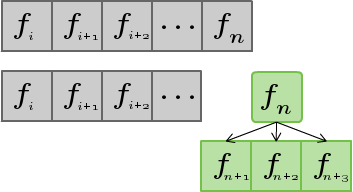
\includegraphics[scale=0.6]{images/DRP-Alg-1.png}
            \end{center}
            \caption{Lista de functores pendientes de ejecución}
        \end{figure}

    Esta reproducción implica por parte de la aplicación la responsabilidad de depositar en \textit{CurrentChildren} los functores
    resultantes de avanzar un paso en la recursión, un mensaje si lo desea y el resultado de la operacion en caso de que el functor llegue
    a un caso base.

    Luego, estos nuevos \textit{``functores hijos''} son agregados a la lista en la parte de atrás. Si los comparamos
    por \textit{``pasos inductivos restantes''} la lista queda ordenada de mayor a menor.\\

        \begin{figure}[!ht]
            \begin{center}
                
\includegraphics[scale=0.6]{images/DRP-Alg-2.png}
            \end{center}
            \caption{Lista de functores ordenada}
        \end{figure}

    Por este orden es que a la hora de delegar trabajo a otro cliente se opta por sacar los functores más a la
    izquierda, aquí se pregunta por la disponibilidad de clientes ociosos y el servidor le dirá de cuantos functores se
    puede desligar. Supongamos que el servidor luego de la petición haya reservado dos clientes, el nodo corriente se
    los enviará y seguirá su ejecución con el resto.\\

        \begin{figure}[!ht]
            \begin{center}
                
\includegraphics[scale=0.6]{images/DRP-Alg-3.png}
            \end{center}
            \caption{Criterio de redistribución}
        \end{figure}

    Cabe aclarar que la complejidad temporal de este algoritmo depende estrictamente del problema particular que se
    corra sobre \rc{}. Sea $f$ la función que representa el comportamiento del algoritmo \ref{Alg-DRP}, $c$ la cantidad máxima de hijos
reproducidos por paso de recursión, $h$ la profundidad máxima del árbol
    de recursión resultante de correr el programa para una entrada particular y $g$ el orden de complejidad de la
    reproducción del functor podemos decir que:

    \begin{table}[ht]
        \begin{center}
        $$T(f(c,h)) = O(\displaystyle\sum\limits_{i=1}^{h} {c^i})*O(g)$$
        \end{center}
    \end{table}

\section{Métricas de Código}

Para analizar el código estáticamente se usaron herramientas como CLOC\footnote{http://cloc.sourceforge.net/} (Count Lines of Code) y
CCCC\footnote{http://cccc.sourceforge.net/} (\textbf{\textit{C}} and \cpp{} Code Counter). En esta sección se describen métricas de
código generales obtenidas por ambas herramientas y se analizan los resultados obtenidos.

\subsection{Métricas de \rc}
\label{recabs_metrics}

\rc{} esta constituido por 23 archivos con un total de 2394 líneas de texto a la fecha de publicación de este documento. La tabla
\ref{cloc_recabs} resume los resultados obtenidos después de correr la herramienta CLOC sobre los archivos fuentes de \rc.

\begin{table}[!htf]
    \begin{center}
    \begin{tabular}{|l|r|r|r|r|c|}
    \hline
    \multicolumn{2}{|c|}{Files} & \multicolumn{3}{|c|}{Line Types} & \hspace{0.2cm}\% \\
    \hline
    \textbf{Type} & \textbf{Count} & \textbf{Blank} & \textbf{Comment} & \textbf{Source} & \small{\textbf{\#Comms./Tot.}}\\
    \hline
    \texttt{C++ source} & 7   &    102  &     301   &    381 & 44.13 \\
    \hline
    \texttt{C++ header} & 16   &    231  &    1010   &    369 &  73.24 \\
    \hline
    \textbf{Total}      &  23  &     333 &     1311  &    750 & 63.6 \\
    \hline
    \end{tabular}
    \caption{Resultados de CLOC para la capa \rc}
    \label{cloc_recabs}
    \end{center}
\end{table}

Los resultados revelan que \rc{} no es un proyecto de gran tamaño. Sin embargo, estas medidas no reflejan su complejidad.

Dijkstra escribió un ensayo muy interesante\cite{ewd1036} donde reflejaba por qué las empresas no deberían considerar las Líneas de Código
como una medida exacta de la productividad del software. Medir la ``productividad de un programador'' en términos del ``número de líneas de
código que produce por mes'' fomenta la escritura de código insípido.

Por otro lado, a mayor número de líneas de código mayor es la complejidad de un producto de software, pero sólo en el sentido de que es
más dificultoso de mantener y comprender, no tiene relación directa con la funcionalidad que éste provee.

Continuando con el análisis sobre los resultados de CLOC, otro dato interesante es la cantidad de líneas de comentarios en el proyecto y su
porcentaje con respecto al total de líneas de código efectivas del proyecto. La siguiente fórmula describe la relación comentarios/código y
la misma fue usada para calcular la última columna de la tabla \ref{cloc_recabs}:

$$\frac{\#comment\_lines}{\#comment\_lines + \#code\_lines}$$

Este valor ronda el 0.63, lo que significa que hay más líneas de comentarios que líneas de código. Este porcentaje de líneas de comentarios
se debe, en mayor medida, a que por cada archivo (por más pequeño que sea) se incluye una cabecera (``header'') definiendo ciertos detalles
del archivo: como sus autores, fecha de creación y la licencia por cual se rige.

Para aún justificar más la alta cantidad de comentarios en \rc, todo componente de software (clases, estructuras, funciones, atributos,
etc.) tiene una descripción detallada a ser interpretada por \textit{Doxygen} (el cuál incluye perfiles de funciones) para la generación de
documentación automática. El ejemplo \ref{recabs_comment} muestra la notación utilizada para Doxygen exhibiendo además el porqué de la alta
tasa de comentarios.

\begin{table}[!h]
    \lstset{language=C++}
    \begin{lstlisting}[frame=single]
/**
 * How many functors are sent to the server ?
 * Should be implemented as a way to distribute work.
 * This function should never return more than n_children-1 and less
 * than 0. In other words, should return a integer k, such that:
 *                     0 <= k < n_children
 *
 * @param n_children : the number of children in the current step.
 * @param depth      : current depth of the recursion tree.
 * @returns the number of children to redistribute.
 */
virtual uint how_much_distribute(uint n_children, uint depth) const = 0;
    \end{lstlisting}
    \centering \caption{Comentario de una función en \rc.}
    \label{recabs_comment}
\end{table}

Por otro lado, el uso extensivo de librerías permitió la minimización de código, el ejemplo exhibido en \ref{using_fud_lib} es un buen
ejemplo para mostrar que en 5 líneas de código, este método inicia el servidor, creando un thread para escuchar paquetes entrantes y varios
otros hilos de ejecución para crear unidades de trabajo y enviarlos a clientes conectados por toda la red, tolerando cortes de
comunicación abruptos y demás funciones que permiten el buen desempeño de distribución de tareas, en resumen, el ahorro de muchas líneas de
código. La librería \fud{} fue la más utilizada en el desarrollo de este proyecto, y en menor medida se utilizó la librería
\textit{\textbf{MiLi}}.

\begin{table}[!h]
    \lstset{language=C++}
    \begin{lstlisting}[frame=single]
void FuDRManager::start()
{
    /* Get the initial packet. */
    Packet initial_packet;
    _server_app.get_initial_packet(initial_packet);

    /* Push initial packet in the stack. */
    push_child(initial_packet);
  
    /* Run the unique DistributableJob. */
    this->run();
    this->wait_completion();    
}
    \end{lstlisting}
    \centering \caption{Ejemplo de uso de la librería \fud}
    \label{using_fud_lib}
\end{table}

En el apéndice \ref{recabs_metrics_report} se muestra un reporte completo sobre las métricas de código de \rc{} generado con la herramienta
CCCC. Incluye muchas métricas de diseño Orientado a Objetos y todo tipo de información relevante en cuanto a código. Un análisis exhaustivo
de los resultados de estas métricas está fuera del alcance de este trabajo. No obstante, el informe proporciona una visión cuidadosa de la
estructura de la librería.

\subsubsection{Cobertura de Código para \rc}
\label{cobertura_recabs}

Es una medida cuantitativa utilizada en pruebas de software que describe el grado de código fuente \textit{testeado}, lo cuál funciona como
una medida indirecta de calidad. En la tabla \ref{recabs_gcov} se muestra la cobertura de código de los archivos de mayor relevancia en
\rc. La cobertura fue hecha corriendo la aplicación \textit{Binary Search} que será introducida en la siguiente sección.

Analizando los resultados de la cobertura de sentencia realizada, más específicamente las líneas no visitadas, sabemos que:
\begin{itemize}
    \item   En el módulo \texttt{DistributionPolicy} las líneas no ejecutadas se deben a que se usa sólo una política de distribución, por
            lo que los demás algoritmos de distribución no son utilizados.
    \item   En el resto de los archivos, las líneas no visitadas corresponden al manejo de errores.
\end{itemize}

La prueba fue realizada con la herramienta \textbf{gcov}\footnote{http://gcc.gnu.org/onlinedocs/gcc/Gcov.html}, corriendo la misma
aplicación 20 veces, variando la cantidad de clientes conectados e interrumpiendo algunos de ellos en su ejecución. En estas pruebas, el
sistema funcionó como se esperaba.

\begin{table}[!htf]
    \begin{center}
    \begin{tabular}{|l|r|r|c|}
        \hline
        & \multicolumn{2}{|c|}{Líneas de código} & Porcentaje \\
        \hline
        \textbf{Archivo} & \textbf{Total} & \textbf{Ejecutado} & \hspace{0.2cm}\textbf{\%} \\
        \hline
        \scriptsize{distributable\_recursive\_processor.cpp} & 91 & 78 & 85.7 \\
        \hline 
        \scriptsize{distribution\_policy.cpp} & 27 & 17 & 62.9 \\
        \hline 
        \scriptsize{by\_size\_result\_sender.cpp} & 18 & 18 & 100 \\
        \hline 
        \scriptsize{fud\_rprocessor.cpp} & 18 & 18 & 100 \\
        \hline 
        \scriptsize{recursion\_manager.cpp} & 37 & 34 & 91.8 \\
        \hline 
        \scriptsize{fud\_rmanager.cpp} & 36 & 35 & 97.2 \\
        \hline 
        \textbf{Total} & 227 & 200 & 88.1 \\
        \hline
    \end{tabular}
    \caption{Resultados de cobertura para los principales archivos de \rc}
    \label{recabs_gcov}
    \end{center}
\end{table}

    \chapter{Aplicación de Prueba \label{chap:dummy_application}}
Con la finalidad de comprobar que \rc{} funciona de la manera esperada, se construyó una aplicación sencilla que use
esta librería. Además
de servir como prueba del software construido, también sirve como ejemplo de elaboración de aplicaciones sobre \rc.

Esta aplicación de prueba utiliza la mayoría de los artefactos de \rc, por lo que su ejecución permitió depurar los errores encontrados en
la etapa de \textit{testing}.

\section{Descripción del Problema}
\label{app_desc_problem}

Dada una lista de números enteros y un número a buscar, se desea saber si este último se encuentra en la lista. La complejidad de este
problema es muy baja, no obstante, lo que se deseaba era observar el comportamiento de la librería y la aplicación en cuanto a:
\begin{itemize}
    \item   distribución de tareas,
    \item   política de distribución sigmoidea,
    \item   fluidez entre servidor y clientes,
    \item   tiempo de corrida de la aplicación distribuida vs. secuencial, y
    \item   performance general del proyecto.
\end{itemize}


\section{Solución}

Esta aplicación, como ya dijimos, se trata de un simple algoritmo de búsqueda, con la particularidad de encontrar una solución que respete
la interfaz que \rc{} propone, y con esto aprovechar el poder de cómputo distribuido en varios nodos de procesamiento. Por ello, la solución
fue planteada siguiendo estos puntos:
\begin{enumerate}
    \item   Crear el \textit{functor} del problema, o sea especificar los atributos necesarios para poder resolver el problema de manera
            aislada. También debemos implementar el algoritmo que dado un functor nos dé $N$ functores hijos, cada uno de ellos más simple
            que el original.
    \item   Dar la implementación de serialización y deserialización del \textit{functor}.
    \item   Crear el \textit{functor} inicial, detallando así el estado del problema original.
    \item   Manejo de resultados.
\end{enumerate}

El algoritmo del punto 1 se realiza de esta manera porque debemos construir una solución que adopte la forma recursiva, ya que la librería
construida lo requiere. Con respecto a los 3 puntos restantes, se deben hacer estas operaciones por separado debido a que algunas serán
responsabilidades del servidor y otras del cliente. El cliente debe saber como un functor se divide en otros functores para llegar tarde o
temprano a los casos bases de cada functor, y por ende, enviar los resultados obtenidos. También debe conocer como se serializan y
deserializan los functores. En cambió, el servidor debe conocer cuál es el functor inicial, ya que es el encargado de iniciar la ejecución,
así como también saber reducir los resultados entrantes.


\subsection{Construcción del \textit{functor}}

Debe reflejar el estado del problema a resolver. En esta aplicación sólo necesitamos tener:
\begin{itemize}
    \item   la lista de números enteros, y
    \item   el número que se desee buscar.
\end{itemize}
Estos atributos son necesarios para solucionar el problema, ambos son requeridos como parámetros de entrada en el algoritmo de búsqueda. El
código fuente en \ref{middle_search} muestra la representación (como clase) creada para este functor, llamada
\texttt{MiddleSearch}.\\

\begin{table}[ht]
    \lstset{language=C++}
    \begin{lstlisting}[frame=single]
/** 
 * Class that represent the Middle Search recursive process.
 */
class MiddleSearch : public recabs::SerializableRecursiveFunctor
{

    public:
        
        typedef std::list<uint32_t> Elements;

        /** Standar constructor
         * 
         * @param v : Container of elements.
         * @param s : Item to search.
         */
        MiddleSearch(Elements& v, uint32_t s);

        /**
         * Destructor.
         */
        ~MiddleSearch(){};

        /**
         * Fills the list with its two children functors if the list
         * contains at least two elements. Otherwise, constructs the
         * corresponding package with the result.
         *
         * @param children : the list of RecursiveFunctor to fill,
         *                   in inductive case.
         * @param result : the packaging result to fill, in base case
         *                 or inductive case.
         *
         */
        virtual void call(ChildrenFunctors& children, Packet& result);

        /**
         * Serializes a MiddleSearch as a packet.
         *
         * @parram packet: Package that will be serialized itself.
         */        
        virtual void serialize(recabs::Packet& pkt);

    private:


        Elements _v;
        uint32_t _searched;

};
    \end{lstlisting}
    \centering
    \caption{Representación del functor}
    \label{middle_search}
\end{table}

La generación de functores hijos a partir de un functor (padre) es una operación de auto-reproduccción, ésto es, dado un functor, ser capaz
de generar functores más pequeños con la finalidad de llegar al caso base en una cantidad finita de ejecuciones por cada functor.

En este caso concreto, de un padre obtendremos dos hijos: un functor que contiene la mitad izquierda de la lista y otro con la derecha. Se
muestra un ejemplo en la figura \ref{functors_division_list} sobre la división de un functor en dos functores hijos.\\

\begin{figure}[ht]
    \begin{center}
        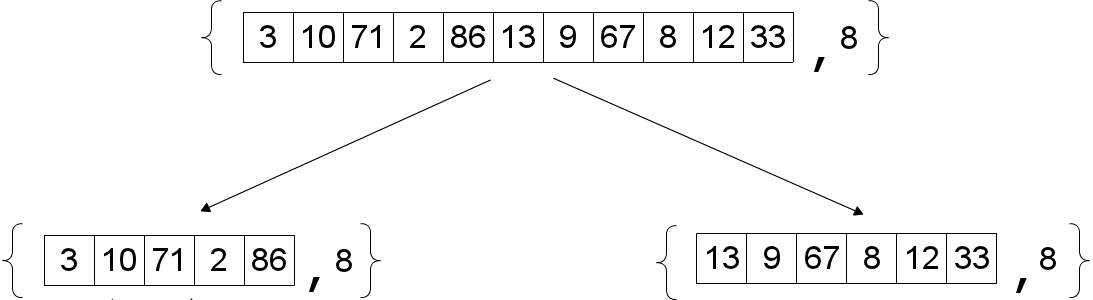
\includegraphics[scale=.35]{images/functors_division_list.png}
        \caption{Auto-reproducción de un functor}
        \label{functors_division_list}
    \end{center}
\end{figure}

El algoritmo utilizado para la división del functor fue el siguiente:
\begin{itemize}
    \item   Casos bases.
            \begin{itemize}
                \item   Si la lista es vacía, se envía un resultado con el valor de verdad \texttt{falso} al servidor.
                \item   Si la lista tiene un sólo elemento, se compara si este elemento es igual al número buscado y se envía el valor de
                        verdad correspondiente al servidor.
            \end{itemize}
    \item   Parte inductiva.
            \begin{enumerate}
                \item   Se descompone la lista de números en dos mitades.
                \item   Con ambas mitades se crean dos nuevos functores, los cuáles representan el mismo problema con diferentes entradas.
            \end{enumerate}
\end{itemize}

El código fuente perteneciente a este algoritmo se encuentra en \ref{call_middle_search}. Para visualizar como continúa la división
de functores del ejemplo graficado en \ref{functors_division_list}, véase la figura \ref{middle_search_tree} que muestra el gráfico
completo sobre la misma lista.

\begin{table}[ht]
    \lstset{language=C++}
    \begin{lstlisting}[frame=single]
void Functor::call(ChildrenFunctors& children, Packet& result)
{
    /* Base case 1 */
    if (_v.empty())
    {
        mili::bostream bos;
        bos << false;
        result = bos.str();
    }

    /* Base case 2 */
    if (uint32_t (_v.size()) == 1)
    {
        mili::bostream bos;
        bos << (_v.front() == _searched);
        result = bos.str();
    }
    /* Inductive case */
    else
    {
        Elements::iterator it = _v.begin();
        advance(it, _v.size() / 2);

        Elements leftChild(_v.begin(), it);
        Elements rightChild(it++, _v.end());

        insert_into(children, new BinarySearch(leftChild, _searched));
        insert_into(children, new BinarySearch(rightChild, _searched));
    }
}
    \end{lstlisting}
    \centering
    \caption{Código para la reproducción de functores}
    \label{call_middle_search}
\end{table}

\subsection{Serialización y Deserialización}

Un functor debe poder serializarse para ser enviado por la red y al llegar a un cliente, éste debe deserializarlo para luego procesarlo.
Para llevar a cabo estas dos operaciones se hizo uso de la librería MiLi\footnote{http://code.google.com/p/mili/}, más específicamente el
módulo \texttt{mili::binary\_streams} el cuál se encarga de crear \textit{streams} binarios con los atributos que tenga el functor.

En \ref{serialize_middle_search} se muestra el código para la serialización  y en \ref{deserialize_middle_search} para la deserialización de
un functor. La serialización consistió en insertar primero la lista de números y luego el número a buscar en la lista. Obviamente cuando
deserializamos hacemos las operaciones inversas al serializado.

\begin{table}[ht]
    \lstset{language=C++}
    \begin{lstlisting}[frame=single]
void Functor::serialize(Packet& pkt)
{
    mili::bostream bos;
    bos << this->_v << this->_searched;
    pkt = bos.str();
}
    \end{lstlisting}
    \centering
    \caption{Serialización del functor}
    \label{serialize_middle_search}
\end{table}

\begin{table}[ht]
    \lstset{language=C++}
    \begin{lstlisting}[frame=single]
void MSDeserializer::deserialize(const Packet& pkt, Functor** rf)
{
    mili::bistream bis(pkt);

    uint32_t searched;
    MiddleSearch::Elements v;
    bis >> v >> searched;
    *rf = new MiddleSearch(v, searched);
}
    \end{lstlisting}
    \centering
    \caption{Deserialización del functor}
    \label{deserialize_middle_search}
\end{table}

\subsection{\textit{Functor} inicial}

Para que el server pueda iniciar la ejecución de la solución, es necesario que disponga del functor inicial, el cuál contiene los datos
originales de entrada, o sea la lista total de números enteros. Para la creación del paquete inicial, primero se debe usar el método
de construcción y luego el de serialización, como se muestra en el código exhibido en \ref{init_middle_search}.

Este aplicación se configuró con un functor inicial que contiene una lista de un millón de números enteros, la cuál es $[0, 1, 2, ...,
999999]$ y el número a buscar es el $-1$.

\begin{table}[ht]
    \lstset{language=C++}
    \begin{lstlisting}[frame=single]
void L4ServerMS::get_initial_packet(Packet& pkt)
{
    MiddleSearch::Elements v;

    for (uint32_t i = 0; i < 1000000; i++)
        mili::insert_into(v, i);

    MiddleSearch b(v, -1);

    b.serialize(pkt);
}
    \end{lstlisting}
    \centering
    \caption{Creación del functor inicial}
    \label{init_middle_search}
\end{table}

\subsection{Manejo de resultados}

El servidor debe tener un algoritmo que maneje los resultados que llegan desde los clientes, los cuáles procesan sus functores y, por
ende, generan y envían estos resultados en base a sus propios cómputos.

En \ref{result_middle_search} se muestra el código fuente que reduce los resultados con la operación lógica \textbf{OR}, debido a que si
\textit{al menos un} functor encuentra el número buscado en la lista, devolveremos {verdadero}. Por contraparte, el número no estará en la
lista si \textit{todos} los functores devuelven el valor de verdad \texttt{falso}.

\begin{table}[ht]
    \lstset{language=C++}
    \begin{lstlisting}[frame=single]
void L4ServerMS::receive_result(const Packet& pkt)
{
    mili::bistream bis(pkt);
    bool res;
    bis >> res;

    _result = (_result || res);
}
    \end{lstlisting}
    \centering
    \caption{Manejo de resultados}
    \label{result_middle_search}
\end{table}


\section{Árbol de functores}
\label{functors_tree}

En toda aplicación podemos ver como los functores forman un árbol que comienza con el functor inicial, luego se van creando los hijos, y
así sucesivamente. Cabe aclarar que cada functor de este árbol va a ser procesado por un cliente en particular, apoyándose en otros
clientes para poder distribuir todos los functores, y así aprovechar al máximo los clientes disponibles del sistema.

En la figura \ref{middle_search_tree} se muestra un ejemplo de árbol de functores para esta aplicación en particular, la cuál tiene como
número a buscar el $8$, y el functor inicial con la siguiente lista: $[3, 10, 71, 2, 86, 13, 9, 67, 8, 12, 33]$.

\begin{center}
    \begin{landscape}
        \begin{figure}[ht]
            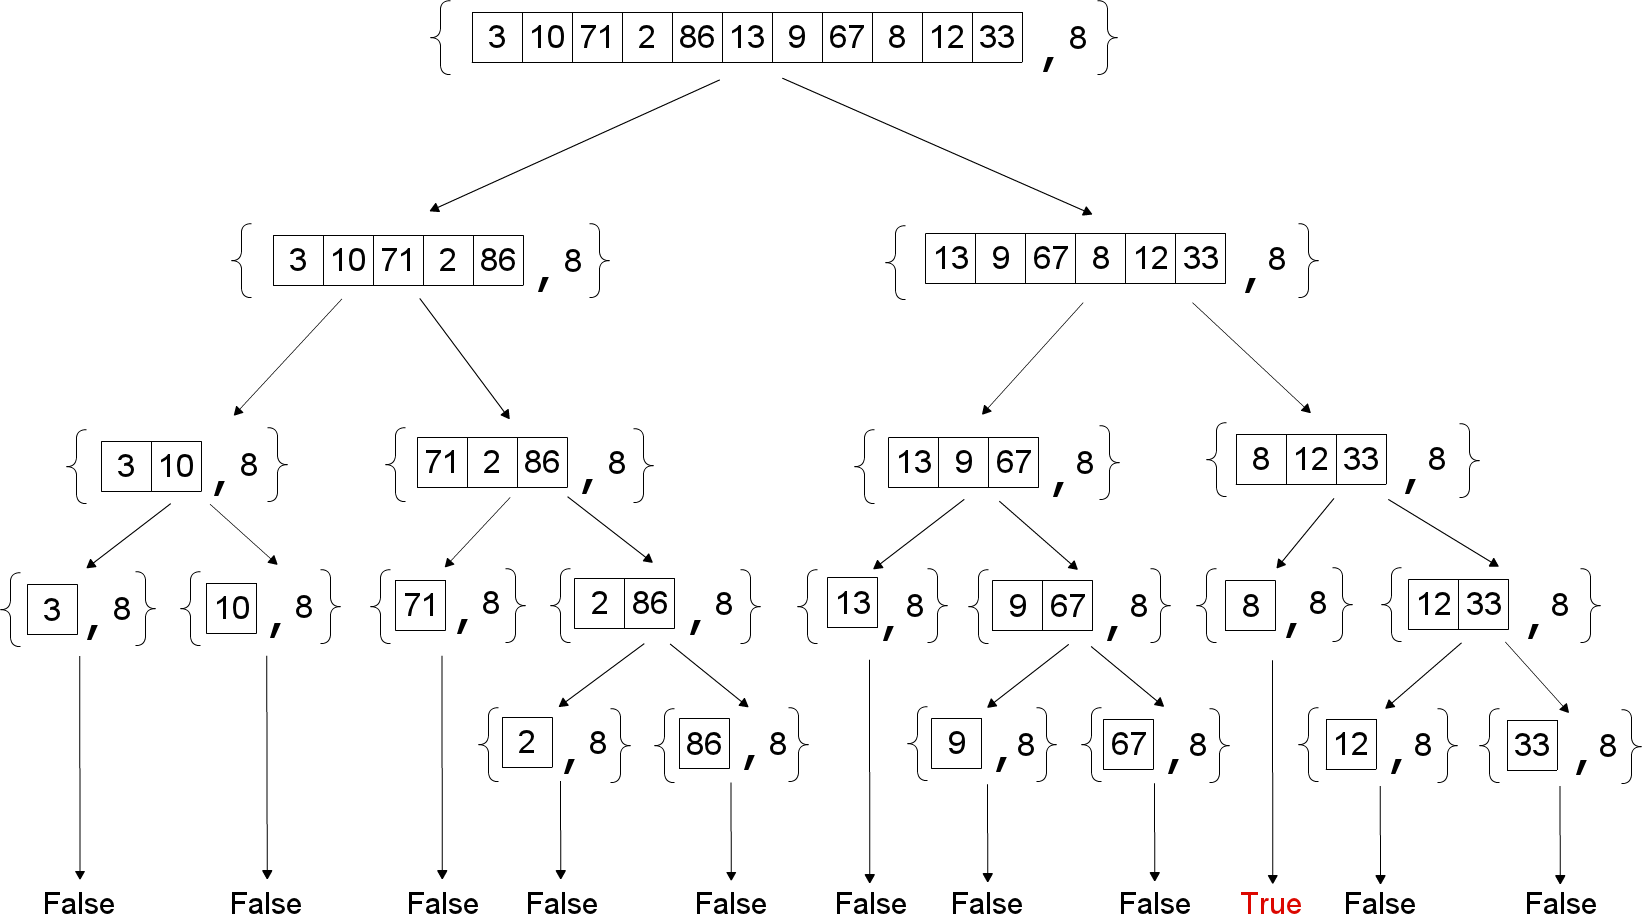
\includegraphics[scale=.37]{images/middle_search_tree.png}
            \caption{Ejemplo de árbol de functores generado por la aplicación de prueba}
            \label{middle_search_tree}
        \end{figure}
    \end{landscape}
\end{center}


\section{Análisis de performance}

Un algoritmo secuencial es usualmente evaluado en términos de su tiempo de ejecución, expresado como una función de su tamaño de entrada. El
tiempo de ejecución de la versión distribuida depende no sólo del tamaño de la entrada sino también del número de nodos usados, y el costo
de comunicación entre nodos.\\

Es importante estudiar la performance de un programa distribuido con el propósito de compararlo con su versión secuencial y así analizar
sus beneficios. Para ello se cuenta con métricas, las cuales nos arrojarán resultados o indicadores sobre el análisis de la performance de
un programa.\\

A continuación mostraremos las principales métricas de este algoritmo de búsqueda distribuido y sus correspondientes análisis, luego de
haber ejecutado el programa con una lista de $10000000$ de elementos con distintas cantidades de nodos de procesamiento. La definición de
estas métricas de rendimiento se encuentran en el libro de \textit{Ian Foster}\cite{parallel}.\\


\subsection{Tiempo de ejecución}

Tiempo de ejecución de un programa: es el intervalo de tiempo desde que el programa se inicia hasta que finaliza. En el caso de
computación distribuida un programa finaliza cuando el último nodo termina su ejecución.

Se denotará el tiempo de ejecución de la búsqueda implementada secuencialmente como $T_s$ y el tiempo de la versión distribuida como
$T_p$. El promedio de $T_s$ en diez ejecuciones fue de $185,77$ segundos.

%BoxPlot
Tomando como muestra diez ejecuciones por misma cantidad de clientes, se confeccionó en el gráfico \ref{execution_boxplot} los
\textit{boxplot's} para uno, dos, tres, cuatro y cinco nodos de procesamiento, respectivamente.
\begin{figure}[!ht]
    \begin{center}
        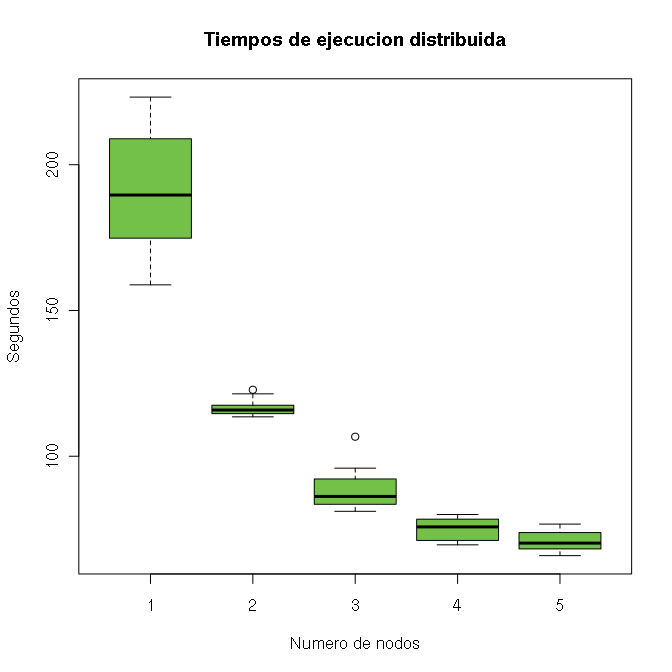
\includegraphics[scale=0.44]{images/execution_boxplot.png}
        \caption{Boxplot's de tiempo de ejecución distribuida}
        \label{execution_boxplot}
    \end{center}
\end{figure}

En la figura \ref{ts_vs_tp} se muestran los tiempos de ejecución promedio para uno a cinco clientes, así como su comparación con el
algoritmo secuencial.
 
\begin{figure}[!ht]
    %Tabla & Grafico
    \begin{minipage}{3cm}
    \begin{flushleft}
    \begin{tabular*}{2,5cm}{c@{\extracolsep{\fill}}c}
        \hline
        \textbf{p} & \textbf{$T_p$} \\ \hline 
        1 & 190,5 \\ \hline
        2 & 116,7 \\ \hline
        3 & 88,6 \\ \hline
        4 & 74,8 \\ \hline
        5 & 70,8 \\ \hline
    \end{tabular*}
    \end{flushleft}
    \end{minipage}
    \    \ \hfill
    \begin{minipage}{12cm}
    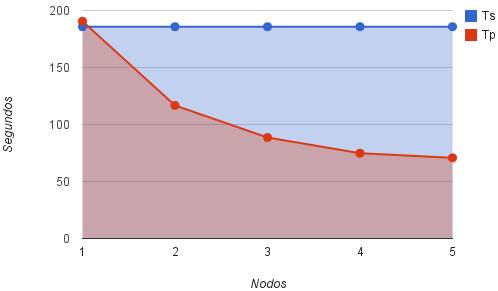
\includegraphics[scale=0.6]{images/ts_vs_tp.png}\\
    \end{minipage}
    \caption{Tiempo secuencial vs. paralelo}
    \label{ts_vs_tp}
\end{figure}

Visto estos resultados, se nota una mejora en rendimiento de tiempo entre la ejecución del programa secuencial y la versión distribuida
ejecutada sobre \rc. Cuando se ejecuta con menos de $3$ nodos (o clientes) podemos decir que el tiempo baja a gran escala pero cuando son
más de $3$, el tiempo de ejecución queda en una meseta.


\subsection{Overhead}

El \textit{overhead} de un programa paralelo es el trabajo adicional que dicho programa realiza respecto a la solución secuencial
equivalente, y se define como: $T_0 = p*T_p - T_s$ .

\begin{figure}[ht]
    %Tabla & Grafico
    \begin{minipage}{3cm}
    \begin{flushleft}
    \begin{tabular*}{2,5cm}{c@{\extracolsep{\fill}}c}
        \hline
        \textbf{p} & \textbf{$T_0$} \\ \hline 
        1  & 4,77 \\ \hline
        2  & 47,65 \\ \hline
        3  & 80,03 \\ \hline
        4  & 113,51 \\ \hline
        5  & 167,98 \\ \hline
    \end{tabular*}
    \end{flushleft}
    \end{minipage}
    \    \ \hfill
    \begin{minipage}{12cm}
    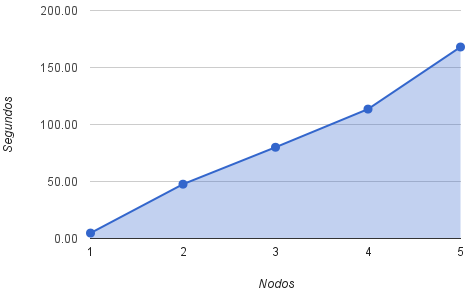
\includegraphics[scale=0.6]{images/overhead.png}\\
    \end{minipage}
    \caption{Overhead}
    \label{overhead}
\end{figure}

En la figura \ref{overhead} vemos que el overhead es directamente proporcional al número de procesadores, lo que indica mismo tiempo de
trabajo adicional por cliente agregado a la ejecución, respecto del algoritmo secuencial.
    

\subsection{Aceleración}

Cuando evaluamos un sistema distribuido, a menudo nos interesa conocer cuánto ganamos en performance paralelizando un algoritmo con respecto
a su implementación secuencial. La aceleración es una medida que arroja el beneficio relativo de resolver un problema en paralelo. Ésta
es definida como la relación del tiempo que toma resolver un problema en un sólo procesador con el tiempo requerido para resolverlo en una
arquitectura paralela con $n$ nodos de procesamiento idénticos. La aceleración se denota con el símbolo $S$ y se define como: $S=T_s/T_p$ .

\begin{figure}[ht]
    %Tabla & Grafico
    \begin{minipage}{3cm}
    \begin{flushleft}
    \begin{tabular*}{2,5cm}{c@{\extracolsep{\fill}}c}
        \hline
        \textbf{p} & \textbf{$S$} \\ \hline 
        1  & 0,97 \\ \hline
        2  & 1,59 \\ \hline
        3  & 2,10 \\ \hline
        4  & 2,48 \\ \hline
        5  & 2,63 \\ \hline
    \end{tabular*}
    \end{flushleft}
    \end{minipage}
    \    \ \hfill
    \begin{minipage}{12cm}
    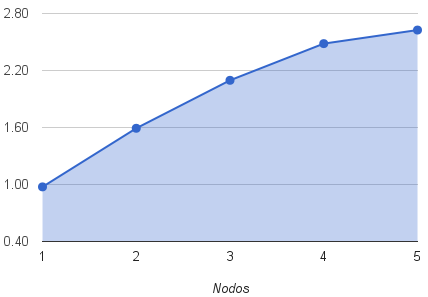
\includegraphics[scale=0.6]{images/speedup.png}\\
    \end{minipage}
    \caption{Aceleración}
    \label{speedup}
\end{figure}

Notemos que en el gráfico \ref{speedup}, la performance de la ejecución paralela aumenta en mayor medida hasta los 3 nodos, y luego el
rendimiento se estabiliza por más nodos que se agregue a la ejecución.


\subsection{Eficiencia}

La eficiencia es una medida que indica la fracción de tiempo útil de un elemento de procesamiento. Se denota con el símbolo $E$ y se
define como: $E = S/p$ .
      
\begin{figure}[ht]
    %Tabla & Grafico
    \begin{minipage}{3cm}
    \begin{flushleft}
    \begin{tabular*}{2,5cm}{c@{\extracolsep{\fill}}c}
        \hline
        \textbf{p} & \textbf{$E$} \\ \hline 
        1  & 0,97 \\ \hline
        2  & 0,80 \\ \hline
        3  & 0,70 \\ \hline
        4  & 0,62 \\ \hline
        5  & 0,53 \\ \hline
    \end{tabular*}
    \end{flushleft}
    \end{minipage}
    \    \ \hfill
    \begin{minipage}{12cm}
    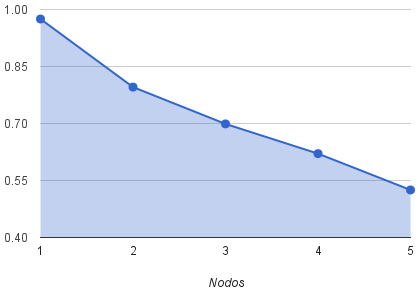
\includegraphics[scale=0.6]{images/eficiency.png}\\
    \end{minipage}
    \caption{Eficiencia}
    \label{eficiency}
\end{figure}

En la figura \ref{eficiency}, vemos que la función de eficiencia decae linealmente, lo que significa una utilidad nodal inversamente
proporcional a la cantidad de nodos procesantes.


\subsection{Costo}
      
El costo de un programa paralelo refleja la suma de los tiempos de ejecución de cada unidad de procesamiento. Se dice que un programa
paralelo tiene costo óptimo si tiene costo computacional igual al programa secuencial. Se define como: $C = p*T_p$ . Esta métrica esta
íntimamente relacionada con la comunicaciones entre los nodos.

\begin{figure}[ht]
    %Tabla & Grafico
    \begin{minipage}{3cm}
    \begin{flushleft}
    \begin{tabular*}{2,5cm}{c@{\extracolsep{\fill}}c}
        \hline
        \textbf{p} & \textbf{$C$} \\ \hline 
        1  & 190,54 \\ \hline
        2  & 233,42 \\ \hline
        3  & 265,80 \\ \hline
        4  & 299,28 \\ \hline
        5  & 353,75 \\ \hline
    \end{tabular*}
    \end{flushleft}
    \end{minipage}
    \    \ \hfill
    \begin{minipage}{12cm}
    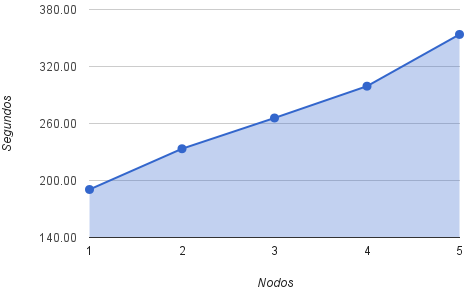
\includegraphics[scale=0.6]{images/cost.png}\\
    \end{minipage}
    \caption{Costo}
    \label{cost}
\end{figure}

En \ref{cost} véase que el costo tiene la misma curva que el overhead salvo el offset del tiempo del algoritmo secuencial. En este ejemplo,
se nota un costo proporcional a la cantidad de nodos.

    \chapter{Proyectos sobre \rc}

Sobre la capa desarrollada pueden ir tanto aplicaciones como otras capas abstractas para la creación de aplicaciones aún más específicas
que se adaptan a otro tipo de características.

A continuación, presentaremos una capa montada sobre \rc{}, la cuál se define para proyectos, en general bioinformáticos. Ademas, será
mencionada una aplicación que corre sobre esta nueva capa, y por lo tanto, también ejecutada bajo \rc.

\section{Motor Combinatorio}

\textbf{\textit{CombEng}} es un motor combinatorio creado también por necesidad de \fude. Constituye una capa más sobre el framework \fud,
más específicamente sobre \rc{}, por lo que también termina siendo un soporte para implementaciones de aplicaciones distribuidas. En la
fundación se presentan, de manera recurrente, problemas de carácter bioinformático, y una familia de ellos se ve caracterizada por compartir
una o más de las siguientes características:
\begin{itemize}
    \item Requerir un motor combinatorio para la generación de árboles de combinaciones.
    \item Utilizar mecanismos de poda sobre dichos árboles.
    \item Requerir un sistema de puntuación por cada una de las combinaciones (\textit{ranking} o \textit{scoring}).
\end{itemize}
Aquellos problemas que comparten al menos una de estas propiedades, es posible atacarlo con el motor combinatorio.

El principal objetivo de este proyecto es crear una capa que permita, a usuarios sin altos conocimientos en programación, implementar
soluciones a este tipo de problemas.

La elección de acoplar \textbf{\textit{CombEng}} como una nueva capa del framework \fud{} en lugar de crear un proyecto aparte, se debió a
que la mayoría de los problemas antes mencionados requieren un elevado nivel de cómputo, lo que en una única computadora se podría lograr
recién en años o siglos.


\subsection{Aplicación \textit{RNA Folding Free Energy}}

En la actualidad, los tratamientos para personas infectadas con \textit{HIV} consisten de una intensiva terapia antirretroviral. Esta
terapia puede ser vista como una sucesión de aplicaciones de antirretrovirales en el tiempo, donde en cada paso de la sucesión se le
suministra al paciente una combinación de uno o más antirretrovirales.

Cuando a una persona se le aplica un antirretroviral, el virus comienza a mutar hasta que logra hacerse resistente. Ésto implica que el
antirretroviral deje de cumplir sus funciones principales y se deba buscar uno nuevo para continuar con el tratamieinto. El orden en que se
aplican los antirretrovirales y cómo éstos son combinados, son factores muy importantes que determinan, entre otras cosas, el tiempo que
transcurrirá hasta el momento en que el virus sea resistente a todos los antirretrovirales.

Hasta el momento, el impacto del escape a los antirretrovirales sobre la estructura secundaria no ha sido estudiada.
\textit{\textbf{RnaFEE}} recopila información sobre como varía la Energía Libre en la estructura secundaria del \textit{RNA} viral a medida
que los antirretrovirales son aplicados sobre la persona infectada.\\

Como el árbol combinatorio a construir posee gran cantidad de nodos y calcular la energía libre de una secuencia es muy costoso, esta
herramienta esta implementada con el motor combinatorio \textit{\textbf{CombEng}} la cual usa \rc{}.


    % Part III
    \part{Refactorización de FuD}
    \label{part:refactorin_fud}

    \chapter{Problema}


\section{\fud{} original}

Como ya dijimos incontables veces, \rc{} se acopló sobre el framework de distribución \fud, el cuál fue desarrollado
íntegramente, como trabajo de tesis, por el Lic. Guillermo Biset y el mismo posee vasta documentación en \cite{clus09}.
En la sección \ref{sec:fud} introducimos esta librería y, en distintas secciones del informe, se fueron aportando datos
importantes de como es su funcionamiento en general.\\

Uno de los principios básicos del funcionamiento de \fud{} se basa en el procesamiento aislado de un cliente, es decir,
un cliente conectado recibe su trabajo, mientras lo realiza ignora cualquier tipo de mensaje que pueda llegar a arriba
desde el servidor. Una vez terminado el trabajo envía el resultado correspondiente al servidor. Luego el servidor,
registra a este cliente como libre, implicando su disponibilidad para un nuevo trabajo. Por lo tanto, la comunicación
entre servidor-cliente consta de solo dos interacciones.\\

En las figuras \ref{FuDServerOrig} y \ref{FuDClientOrig} se muestra un diagrama de actividad de la dinámica de los
componentes más importantes de \fud{} original tanto de lado servidor como de cliente respectivamente. Cabe destacar
que en ellos se obviaron aspectos de concurrencia con el fin de no dificultar la visualización el diagrama, se muestra
un solo hilo de ejecución donde un servidor envía un trabajo a un nodo y solamente espera de él su resultado
correspondiente.

    \begin{figure}[ht]
        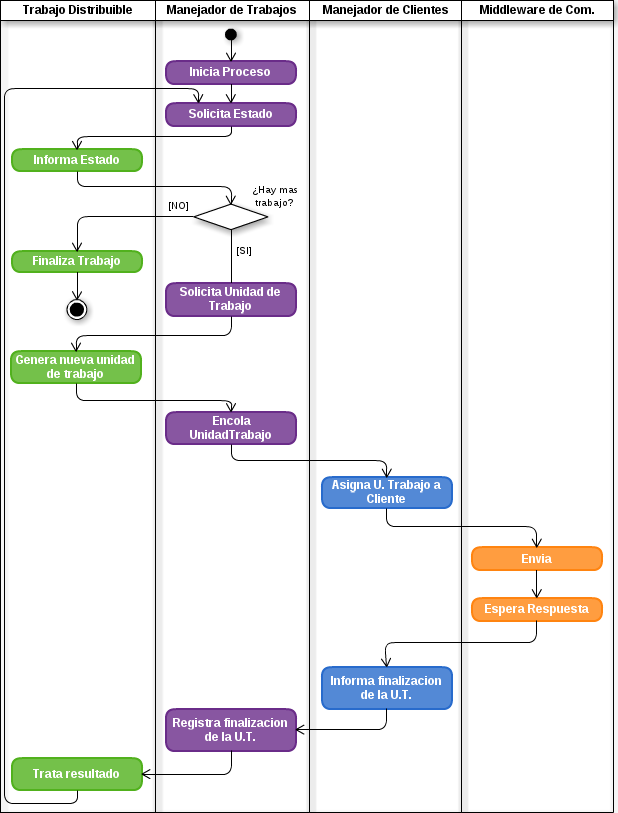
\includegraphics[scale=0.65]{images/ActivityFuDServer-Orig.png}
        \caption{Diagrama de Actividad de \fud{} versión original lado servidor}
            \label{FuDServerOrig}
    \end{figure}

    \begin{figure}[ht]
        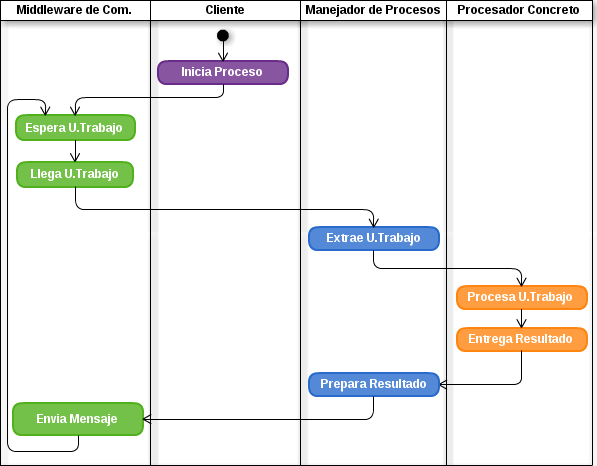
\includegraphics[scale=0.70]{images/ActivityFuDClient-Orig.png}
        \caption{Diagrama de Actividad de \fud{} versión original lado cliente}
            \label{FuDClientOrig}
    \end{figure}



\section{Descripción del Problema}

\rc{} requiere interacción entre servidor y cliente en el transcurso del procesamiento de un trabajo. Ésto se debe a que la generación de
nuevas unidades de trabajo depende exclusivamente de la distribución de trabajo no computado por parte de los clientes, disminuyendo su
carga de trabajo. Un cliente antes de delegar trabajo al servidor necesita también una comunicación previa para conocer si
el servidor tiene disponibilidad de clientes ociosos. Además \rc{} permite el envío de resultados y mensajes en cualquier momento.

Por la naturaleza de \fud{} original era imposible disponer con esta interactividad para poder llevar acabo todas las operaciones antes
descritas, razón que motivó a la refactorización del framework.


    \chapter{Solución}

El rediseño de software llevado a cabo mantiene el diseño original del framework, agregándole nuevas funcionalidades para brindar
interactividad entre servidor y cliente de manera que \rc{} puede acoplarse a él. Ésto permite que aplicaciones que corrían sobre \fud{}
original sigan haciéndolo, con la opción a usar las nuevas características que serán presentadas a continuación.

\section{Nuevas funcionalidades}

Concretamente, las funcionalidades requeridas por \rc{} que forman parte del rediseño del framework son:
\begin{itemize}
    \item   envío de mensajes de cliente a servidor, y
    \item   pedido y reserva de clientes.
\end{itemize}
A continuación veremos, en detalle, cada uno de ellos.

\subsection{Envío de mensajes}

La importancia de este punto es la libertad que el cliente obtiene pudiendo enviar mensajes cuando desee y, así, el servidor por ejemplo
poder ir reduciendo resultados o conocer del estado de cada cliente, sin que éstos dejen de procesar su trabajo asignado.

Ya que en \fud{} original el cliente sólo enviaba un resultado al fin del procesamiento, ésto significaba que el cliente había terminado de
ejecutar su tarea. Con la implementación de esta nueva funcionalidad, se debió añadir un paquete que informa que una unidad de trabajo ha
finalizado y por ende, el cliente que lo envió es libre nuevamente.

A continuación se dan las responsabilidades que deben atender tanto el cliente como el servidor:
\begin{itemize}
    \item   \underline{Cliente}\\Permitir que el cliente envíe mensajes en cualquier momento y la cantidad de veces que desee, sin necesidad
            de cortar su ejecución. Cuando termine de ejecutar su unidad de trabajo, debe enviar el paquete de finalización.
    \item   \underline{Servidor}\\Permitir que el servidor reciba cualquier cantidad de mensajes de un cliente en particular, y recién
            marcarlo como un cliente ocioso y a su trabajo asigando como finalizado cuando éste le envíe un paquete de finalización.
\end{itemize}


\subsection{Pedido y reserva de clientes}

Un cliente podrá saber sobre la disponibilidad de clientes ociosos, y más aún podrá reservar una cantidad para su uso. El uso de esta
funcionalidad trae aparejado una mayor responsabilidad para los clientes, ya que su utilización en demasía sobrecarga al servidor de
consultas, con ello disminuye demasiado la cantidad de clientes libres del framework y, por lo tanto, la performance total del proyecto
podría decaer drásticamente.

Las responsabilidades de los dos actores de esta comunicación son:
\begin{itemize}
    \item   \underline{Cliente}\\Otorgar la posibilidad de que el cliente pregunte al servidor sobre la disponibilidad de clientes libres
            y espere una eventual respuesta del servidor. Será el número de clientes ociosos que el servidor desee designar en un momento
            dado, quedando así reservados a merced del cliente que realizó la pregunta.
    \item   \underline{Servidor}\\Debe recibir la consulta por clientes libres, calcular el número de clientes ociosos que desee enviar
            como respuesta, y en caso de que el número fuera positivo, reservará esa cantidad de clientes no pudiendo ser usados durante
            un tiempo estipulado.
\end{itemize}

Este \textit{feedback} entre cliente y servidor le permite a \rc{} redistribuir los functores hijos de un cliente a otros clientes ociosos
con el fin de balancear la carga de trabajo, y así lograr un alto rendimiento en la ejecución de aplicaciones. En otras palabras, permite
generar unidades de trabajo a demanda, asegurándose que existen clientes libres para procesar estas tareas.

 
\section{Diseño}
\label{redesign_design}

Como se dijo anteriormente, se mantuvo el diseño original del framework, no hubo cambios radicales, salvo la inclusión de dos nuevas clases
y la modificación de, alrededor, 10 clases que permitieron la implementación de las nuevas funcionalidades. Por lo tanto, esta
refactorización de \fud{} no cambia en líneas generales el diagrama de clases, el cuál se puede visualizar en la figura
\ref{fud_class_diagram}.

Para ver cómo funciona el nuevo \fud{} refactorizado, a continuación se encuentran las figuras \ref{FuDServerDuplex} y
\ref{FuDClientDuplex}, las cuáles ilustran la dinámica de comportamiento tanto del servidor como del cliente, respectivamente. Estos
gráficos pueden ser contrastados con las figuras \ref{FuDServerOrig} y \ref{FuDClientOrig}, las cuáles son los diagramas pertenecientes al
viejo esquema de actividades de \fud{} original.

\begin{figure}[ht]
    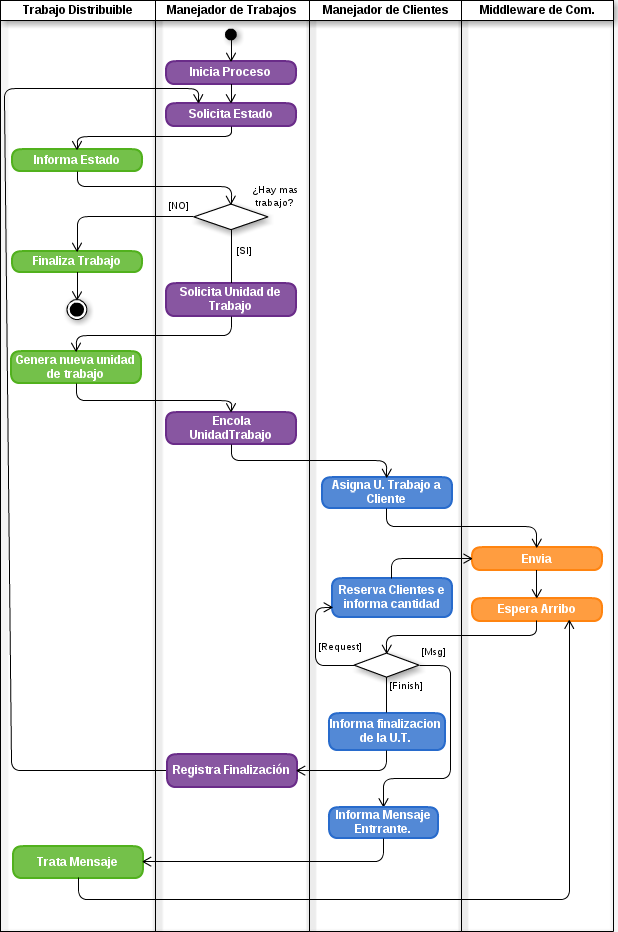
\includegraphics[scale=0.65]{images/ActivityFuDServer-Duplex.png}
    \caption{Diagrama de Actividad de \fud{} refactorizado lado servidor}
    \label{FuDServerDuplex}
\end{figure}

\begin{figure}[ht]
    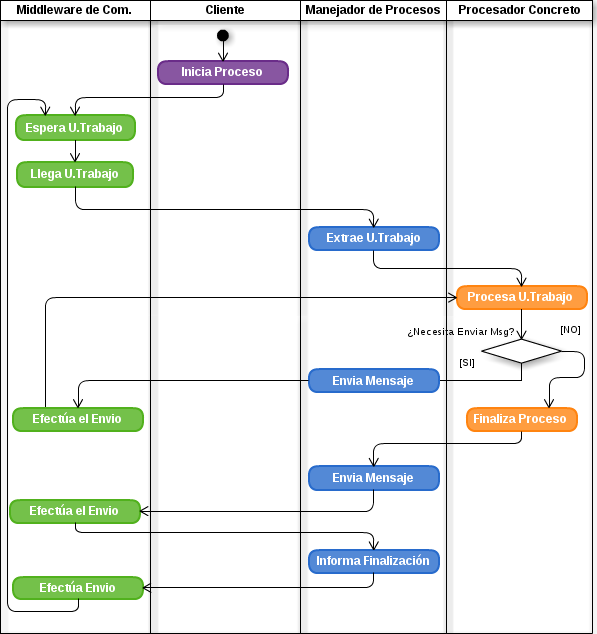
\includegraphics[scale=0.70]{images/ActivityFuDClient-Duplex.png}
    \caption{Diagrama de Actividad de \fud{} refactorizado lado cliente}
    \label{FuDClientDuplex}
\end{figure}

\begin{center}
    \begin{landscape}
        \begin{figure}[ht]
            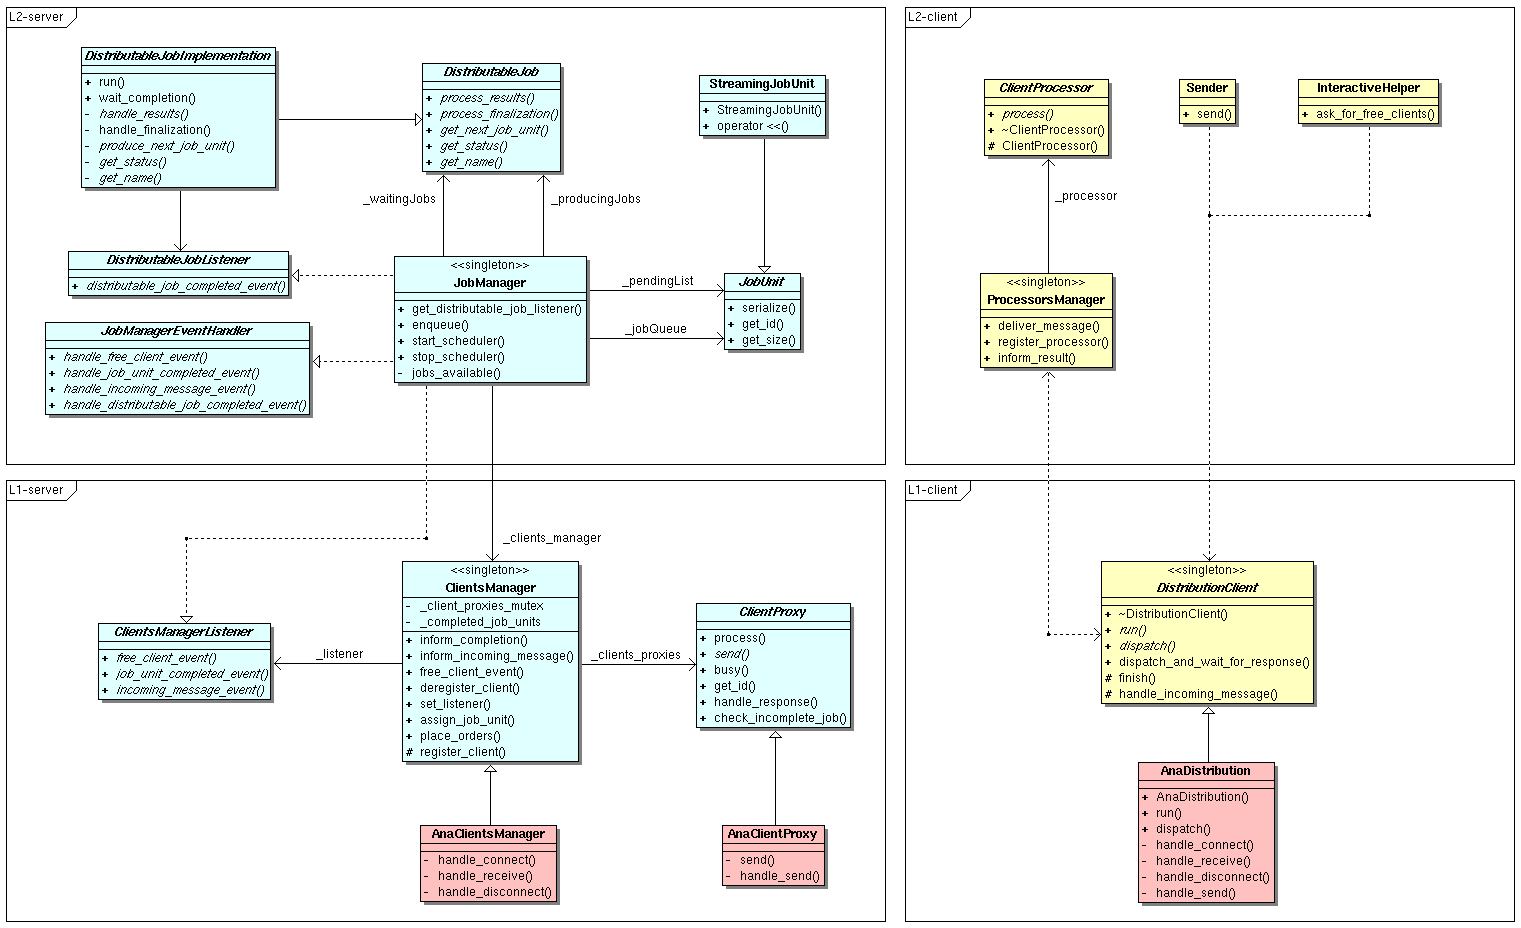
\includegraphics[scale=.38]{images/fud_class.png}
            \caption{Diagrama de clases de \fud{} refactorizado}
            \label{fud_class_diagram}
        \end{figure}
    \end{landscape}
\end{center}


\subsection{Sender}

Se creó esta nueva clase con el simple propósito de servir al cliente con una interfaz para el envío de mensajes. Véase figura
\ref{fud_sender}.

\begin{figure}[ht]
    \begin{center}
        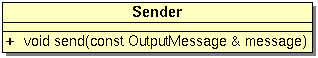
\includegraphics[scale=.75]{images/fud_sender.png}
        \caption{Clase \texttt{Sender}.}
        \label{fud_sender}
    \end{center}
\end{figure}

Este componente tiene una relación directa con la capa L1, encargada de la comunicación con el servidor. El método \texttt{send} adosa, al
mensaje que se desee enviar, un encabezado indicando la presencia de mensaje regular.

\subsection{Ayudante de interactividad}

Este módulo es el encargado de iniciar el pedido y reserva de clientes, por lo que es el artefacto que deben utilizar los clientes de una
aplicación que deseen optar por la reserva de clientes ociosos. Véase figura \ref{fud_interactive_helper}.

\begin{figure}[ht]
    \begin{center}
        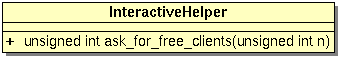
\includegraphics[scale=.75]{images/fud_ihelper.png}
        \caption{Clase \texttt{InteractiveHelper}.}
        \label{fud_interactive_helper}
    \end{center}
\end{figure}

El método \texttt{ask\_for\_free\_clients} toma un número entero, el cuál es el número de clientes deseados por el cliente, luego envía
este requerimiento al servidor, éste calcula, en base al número y la cantidad de clientes ociosos que posee, cuántos clientes le puede
destinar al requeridor. Finalmente, el cliente recibe el número de clientes ociosos que el servidor le pudo asignar. En la figura
\ref{place_orders} se muestra un diagrama de actividad sobre esta interacción de pedido y reserva de clientes.

\begin{figure}[ht]
    \begin{center}
        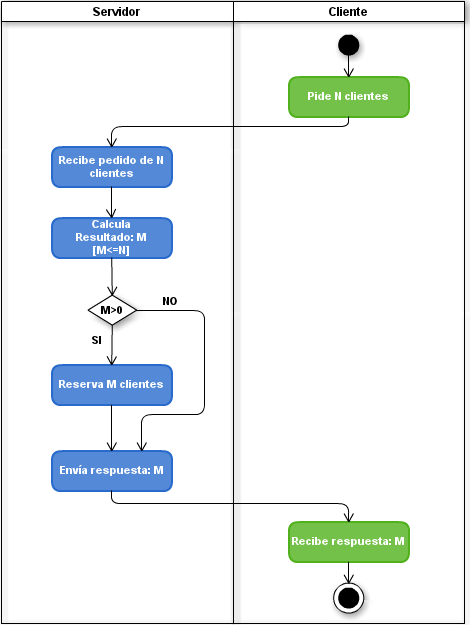
\includegraphics[scale=.65]{images/place_orders.png}
        \caption{Diagrama de actividad de pedido y reserva de clientes}
        \label{place_orders}
    \end{center}
\end{figure}


\section{Implementación}

Como se dijo en la parte de Diseño \ref{redesign_design}, se modificó más de lo que se añadió, por lo que también en lo que respecta a
código, fueron más las líneas aportadas para la adaptación de las nuevas funcionalidades que la implementación de estas nuevas
características en sí.

\subsection{Cambios en \fud}

Aquí hablaremos de los cambios sustanciales que sufrió este software para poder adoptar las nuevas características. Nombraremos las
modificaciones siguiendo la arquitectura cliente/servidor, empezando por los nuevos encabezados de mensaje que se incluyeron, y en cada caso
los servicios que se refactorizaron.

\subsubsection{Servidor}

Los siguientes \textit{headers} corresponden a paquetes enviados de \textbf{clientes al servidor}:
\begin{itemize}
    \item   \texttt{kMessage} : mensaje que será tratado por la aplicación que corra sobre \fud.
    \item   \texttt{kFreeClientsRequest} : usado para pedido y reserva de clientes ociosos.
    \item   \texttt{kJobUnitCompleted} : paquete que informa la finalización de una unidad de trabajo.
\end{itemize}

Cabe destacar que \texttt{kMessage} es el único tipo de mensaje que maneja la aplicación L3, generalmente para resultados y mensajes
intermedios, ambos tratados de la manera que el usuario del framework disponga.

En el caso de un pedido de clientes libres, el servidor cuenta con un \textit{handler} que retorna el número de clientes que dispone para
tal pedido. Para ello, se lleva rastro de todas las reservas hechas de todos los clientes, lo cuál otorga una visión general que permite
obtener el número de clientes realmente disponibles (no reservados) en un momento dado. La respuesta debió ser lo más exacta posible, debido
a que un error en ella se traduce a una ``falsa'' prestación de recursos, y debió ser rápida ya que cuando un cliente realiza esta consulta,
espera una respuesta por parte del servidor sin poder seguir procesando su tarea.

Para incluir el fin de una unidad de trabajo, sólo se tuvo que agregar un nuevo evento que atendiera esta acción. La finalización de un
trabajo puede tener una implementación específica a la aplicación.

\subsubsection{Cliente}

Por otra parte, los mensajes que viajan desde el \textbf{servidor hacia los clientes} pueden ser:
\begin{itemize}
    \item   \texttt{kJob} : representa una unidad de trabajo que ha sido asignada al destinatario.
    \item   \texttt{kFreeClientsResp} : respuesta al pedido de clientes ociosos.
\end{itemize}

El tratamiento de la llegada de una unidad de trabajo esta contemplada en el \fud{} original. La inclusión del manejo a la respuesta del
pedido de clientes trajo aparejada la implementación de una espera bloqueante sobre el cliente, ya que éste no puede seguir procesando su
trabajo pendiente sin una respuesta.


\subsection{Métricas de la refactorización de \fud}

Para analizar el código estáticamente se usaron herramientas como CLOC\footnote{http://cloc.sourceforge.net/} (Count Lines of Code) y
CCCC\footnote{http://cccc.sourceforge.net/} (\textbf{\textit{C}} and \cpp{} Code Counter). En esta sección se describen métricas de
código generales obtenidas por ambas herramientas y se analizan los resultados obtenidos.

El rediseño del framework \fud{} fue realizado con 21 modificaciones de archivos más la creación de otros 5 archivos con un total de 1114
líneas de texto. La tabla \ref{cloc_redesign_fud} resume los resultados obtenidos después de correr CLOC sobre los archivos fuentes.

\begin{table}[!htf]
    \begin{center}
    \begin{tabular}{|l|r|r|r|r|r|c|}
    \hline
    \multicolumn{3}{|c|}{Files} & \multicolumn{3}{|c|}{Line Types} & \hspace{0.2cm}\% \\
    \hline
    \textbf{Type} & \textbf{Mod.} & \textbf{Cre.} & \textbf{Blank} & \textbf{Comment} & \textbf{Source} &
\small{\textbf{Com./Tot.}}\\
    \hline
    \texttt{C++ source} & 9   & 3   &    60  &    176   &   287 & 38.01 \\
    \hline
    \texttt{C++ header} & 12  & 2   &    88  &    403   &   100 & 80.11 \\
    \hline
    \textbf{Total}      & 21  & 5   &   148  &    579   &   387 & 59.93 \\
    \hline
    \end{tabular}
    \caption{Resultados de CLOC para el refactorización de \fud}
    \label{cloc_redesign_fud}
    \end{center}
\end{table}

Haciendo referencia en la sección ``Métricas de \rc''(véase \ref{recabs_metrics}), se dijo que las líneas de código no reflejan la
productividad, más aún que a mayor líneas más complejo es el producto de software, y por lo tanto es más difícil de mantener y comprender.
En lo que respecta a la refactorización de \fud, puede verse que con sólo 387 líneas de código se desarrollaron las nuevas funcionalidades,
que resultaron funcionar como se esperaba.

Como ocurrió en el desarrollo de \rc, existen más líneas de comentario que líneas de código, con una relación de casi 60\%. Esto indica que
se hizo hincapié en la documentación para el mejor entendimiento futuro del funcionamiento del framework. Esta cantidad de comentarios se
deben en gran medida a los encabezados de cada archivo y al uso Doxygen, como ya se explicó en la sección sobre las métricas de \rc.

En el apéndice \ref{fud_metrics_report} se muestra un reporte completo sobre las métricas de código de \fud{} después de su
refactorización, generado con la herramienta CCCC. Incluye muchas métricas de diseño Orientado a Objetos y todo tipo de información
relevante en cuanto a código. Un análisis exhaustivo de los resultados de estas métricas está fuera del alcance de este trabajo. No
obstante, el informe proporciona una visión cuidadosa de la estructura de la librería.

    \chapter{Dependencias externas}

\section{ANA}
\ana{} (acrónimo de \textit{Asynchronous  Network API}) es una API diseñada para permitir desarrollar
aplicaciones de red con una arquitectura cliente/servidor.
Para implementar esta funcionalidad, la API utiliza un modelo asíncrono (es decir, sin bloqueo de operaciones). De esta
manera, el desarrollador no necesita enfocarse con detalles de código relevante a la comunicación, pudiendo
concentrarse en otras funcionalidades relacionadas con el programa.\\

Se cuenta con una implementación\footnote{http://code.google.com/p/ana-net/} de esta API usando
Boost.Asio\footnote{http://www.boost.org/doc/libs/1\_48\_0/doc/html/boost\_asio.html} (Librería de red multiplataforma)
que logra explotar todo el potencial de la librera brindando una nueva API externa que simplifica su uso y permite al
usuario final mediante la implementación de unos pocos \textit{handlers} tener una aplicación con comunicación
asíncrona.\\


En la primera versión de \fud{} se contaba con una capa de comunicación (Véase \ref{fud-layers}) realizada con
Boost.Asio. Tenía la particularidad de ser bloqueante, es decir, una vez recibido un mensaje, el cliente desoye todo
mensaje del servidor hasta que termina con su trabajo donde retorna a esperar nuevos mensajes. Luego se contó con una
reimplementación de esta capa que usa como librería de red a \ana. Esta nueva \textit{Layer 1} otorga un código más
limpio y
legible con las mismas funcionalidades que el anterior.\\

\fud/\ana{} fue de vital importancia para lograr la refactorización de \fud{} antes descrita, ya que al usar a \ana{}
se simplifico el uso de mensajería asíncrona necesaria para el envío de mensajes y resultados entre cliente y
servidor. Como un todo un mecanismo concurrente que opera las distintas envíos y escuchas permitió mediante
la agregación de algunos métodos lograr tener interacción entre cliente y servidor en cualquier momento del
procesamiento.



    % Part IV
    \part{Conclusión}
    \label{part:conclusion}

    \chapter{Conclusión}
\label{chap:conclusion}

Con respecto a \rc{} se ha obtenido una abstracción como una nueva capa del framework \fud{} que agrupa las soluciones más recurrentes a 
problemas bioinformáticos que existen en \fude. Más específicamente, se logró definir una librería que tome como entrada la solución
recursiva a cualquier problema con subproblemas sin superposición teniendo como resultado una versión distribuida de la misma.
El trabajo realizado ha arrojado resultados de performance positivos tanto con la aplicación trivial presentada como así también con
\textit{RNAFoldingFreeEnergy} sobre el motor combinatorio \textit{CombEng}.

En relación a la refactorización de \fud{}, se obtuvo una nueva versión del framework, que cumpliendo con sus principios básicos y
manteniendo su eficiencia, permite realizar interacciones entre los clientes y el servidor. Ahora, admite un conjunto más amplio de
posibles problemas a resolver.

Este proyecto, aporta una herramienta fundamental para la futura resolución de problemas que afronte \fude{} para obtener resultados
concretos a corto plazo. Ambos resultados han cumplido con todas las expectativas y han cubierto cada uno de los objetivos
planteados desde el inicio de este proyecto.     

    \chapter{Trabajos futuros}
\label{chap:future_work}

Tal vez la parte más importante sobre \rc{} es lo que se haga con ella, es por eso que a continuación se presentará una lista con proyectos
a futuro, los cuáles serán montados sobre la capa desarrollada. Además, existen funcionalidades y/o extensiones de este trabajo que serán
dejadas como futuras tareas de la fundación. He aquí algunos trabajos interesantes por llevar a cabo:
\begin{itemize}
    \item   Implementar proyectos bioinformáticos. Un caso concreto es \textit{backbones-generator}, este proyecto pertenece a \fude{} y
            tiene como objetivo construir una base de datos de esqueletos (\textit{backbones} o cadenas proteicas principales) de un tamaño
            dado a partir de una combinatoria de ángulos y restricciones. Se encuentra implementado secuencialmente, y se desea construir la
            versión \rc{} del mismo problema.
    \item   Adaptar esta capa para que proyectos \textbf{\textit{BOINC}} funcionen sobre ella. Lo que se debe hacer es distribuir los
            functores recursivos, como unidades de trabajo, entre los nodos conectados de la forma en que este middleware trabaja. El uso
            de \textbf{\textit{BOINC}} permitiría a \fude{} obtener la potencia de procesamiento de miles de CPUs en proyectos científicos.
    \item   Construir nuevas políticas de distribución para un balanceo de carga específico sobre determinadas aplicaciones o para
            definir un balanceo genérico con buen rendimiento sobre un grupo de problemas afines. En muchos casos, una \textit{buena}
            distribución depende exclusivamente del problema que deseamos resolver, es por esto que se pueden extender políticas para
            una necesidad concreta. Por el contrario, también es posible crear mecanismos de balanceo de carga que ataquen a un conjunto de
            aplicaciones, y mantengan una buena performance en todos los casos.
\end{itemize}


    % Bibliography
    \addcontentsline{toc}{chapter}{Bibliografía}
    \bibliographystyle{annotate}
    \bibliography{biblio}

    % Appendix
    \appendix \label{appendix}
    \addappheadtotoc
    \appendixpage
    \newpage

    \chapter{Patrones De Diseño}
	\section{Qué Son Los Patrones De Diseño}
Los patrones de diseño son la base para la búsqueda de soluciones a problemas comunes en el desarrollo de software y
otros ámbitos referentes al diseño de interacción o interfaces. Un patrón describe un problema que ocurre varias
veces en un sistema, y la base de la solución a ese problema. Los patrones de diseño son el resultado del consenso de
los profesionales en el área y brindan herramientas a los diseñadores de sistemas para no escoger malos caminos,
valiéndose de documentación disponible en lugar de simplemente la intuición.

    \section{Patrones}
Un patrón de diseño es una solución a un problema de diseño. Para que una solución sea considerada un
patrón debe poseer ciertas características. Una de ellas es que se debe haber comprobado su efectividad resolviendo
problemas similares en ocasiones anteriores. Otra es que debe ser reusable, lo que significa que es aplicable a
diferentes problemas de diseño en distintas circunstancias. Cada patrón de diseño se focaliza sobre un problema o issue
particular de diseño (DOO).

En general, un patrón tiene cinco elementos esenciales:
        \begin{enumerate}
            \item \textbf{El nombre del patrón} nombre estándar del patrón por el cual será reconocido en la comunidad
(normalmente se expresan en inglés), se usa para describir un problema de diseño, su solución, y consecuencias.

            \item \textbf{Tipo} Clasificación en la que se encuentra el patrón, éstos pueden ser:
                \begin{itemize}
                    \item \textit{Creacionales}:Muestran la guía de cómo crear objetos cuando
sus creaciones requieren tomar decisiones. Estas decisiones normalmente serán resultas dinámicamente decidiendo que
clases instanciar o sobre que objetos un objeto delegará responsabilidades
                    \item \textit{Estructurales}: Describen la forma en que diferentes tipos de
objetos pueden ser organizados para trabajar unos con otros
                    \item \textit{Comportamiento}: Se utilizan para organizar, manejar y combinar comportamientos
                \end{itemize}

            \item \textbf{El problema} describe cuando aplicar el patrón, explica el problema y su contexto. También
                describe problemas de diseño específicos tales como ``Como representar un algoritmo como un objeto''.
                Además, describe la estructura de clases y objetos que son sintomáticas de un diseño inflexible. A
                veces, el problema puede incluir una lista de condiciones que deben ser reunidas antes de que tenga
                sentido aplicar el patrón. \item \textbf{La solución} describe los elementos que integran el
                diseño, sus relaciones, responsabilidades y colaboración. La solución no describe un diseño
                particular concreto o implementación, porque un patrón puede ser aplicado en muchas situaciones
                diferentes. De hecho, el patrón provee una descripción abstracta de un problema de diseño y
                como una disposición general de los elementos lo resuelve.
            \item \textbf{Las consecuencias} son los resultados y compromisos de aplicar el patrón. Estas son
                fundamentales para evaluar alternativas de diseño y para la comprensión de los costos y
                beneficios de aplicar el patrón. Las consecuencias de un patrón incluye su impacto sobre la
                flexibilidad del sistema, expansión o portabilidad.
        \end{enumerate}

	\section{Patrones Utilizados En \rc{}}
        A lo largo del proceso de diseño se encontraron problemas que coincidían con patrones. Estos patrones se
        explican brevemente a continuación:

        \subsection{Chain of Responsibility}\label{chain_pattern}
Proporcionar a más de un objeto la capacidad de atender una petición, para así evitar el acoplamiento con el que objeto
que hace la petición. Se forma con estos objetos una cadena, en la cual cada objeto o satisface la petición o la pasa al
siguiente.



    \subsubsection{Aplicabilidad}
        Este patrón es usado cuando:
        \begin{itemize}
            \item Hay más de un objeto que pueden manejar una petición, y el manejador no se conoce a priori, sino que
                debería determinarse automáticamente.
            \item Se quiere enviar una petición a un objeto entre varios sin especificar explícitamente el receptor.
            \item El conjunto d objetos que pueden tratar una petición debería ser especificado dinámicamente.
        \end{itemize}

    \subsubsection{Participantes}
        Entidades que forman parte del patrón.
        \begin{itemize}
            \item \textit{Client}: será el encargado de generar las peticiones que hayan de pasar por el manejador
                genérico.
            \item \textit{Handler}: deberá  estar  compuesto  por  un  interfaz  donde  se vayan a desarrollar las
                    peticiones que genera el cliente.
            \item \textit{Concrete Handler}: tratará  la  petición  que  le  corresponda del cliente según su criterio.
        \end{itemize}

    \subsubsection{Estructura}

    \begin{figure}[!h]
        \centering
        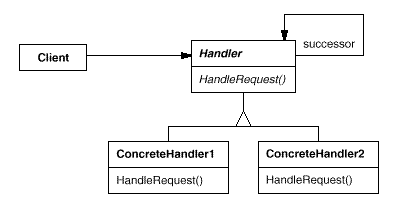
\includegraphics[scale=0.8]{images/chain-of-responsibility}
        \caption{Patrón \textit{``Chain of Responsibility''}.} \label{chain_pattern_img}
    \end{figure}
    \chapter{Reporte de métricas de código de \rc}
\label{recabs_metrics_report}

\begin{tabular}{|c|l|}
\hline
\multicolumn{2}{|c|}{CCCC Software Metrics Report generated Tue Nov 22 20:34:56 2011} \\
 \hline 
 \textbf{Project}       & Summary table of high level measures summed over all\\
 \textbf{Summary}       & files processed in the current run.  \\
 \hline 
 \textbf{Procedural}    & Table of procedural measures (i.e. lines of code, \\
 \textbf{Metrics}       & lines of comment, McCabe's cyclomatic complexity \\
 \textbf{Summary}       & summed over each module.  \\
 \hline 
 \textbf{Object Oriented} & Table of four of the 6 metrics proposed by Chidamber \\
 \textbf{Design}        & and Kemerer in their various papers on 'a metrics suite \\
                        & for object oriented design'. \\
 \hline 
 \textbf{Structural}    & Structural metrics based on the relationships of each \\
 \textbf{Metrics}       & module with others. Includes fan-out (i.e. number of \\
 \textbf{Summary}       & other modules the current module uses), fan-in (number \\
                        & of other modules which use the current module), and \\
                        & the Information Flow measure suggested by Henry and \\
                        & Kafura, which combines these to give a measure of \\
                        & coupling for the module. \\
 \hline 
 \textbf{Other Extents} & Lexical counts for parts of submitted source files which \\
                        & the analyser was unable to assign to a module. Each \\
                        & record in this table relates to either a part of the \\
                        & code which triggered a parse failure, or to the residual \\
                        & lexical counts relating to parts of a file not \\
                        & associated with a specific module. \\
 \hline 
 \textbf{About CCCC}    & A description of the CCCC program.  \\
 \hline 

\end{tabular}

\section{Project Summary}
 This table shows measures over the project as a whole. \begin{itemize}
\item NOM = Number of modules\\ 
 Number of non-trivial modules identified by the analyser. Non-trivial modules include all classes, and any other module for which member
functions are 
identified. 
\item LOC = Lines of Code\\ 
 Number of non-blank, non-comment lines of source code counted by the analyser. 
\item COM = Lines of Comments\\ 
 Number of lines of comment identified by the analyser 
\item MVG = McCabe's Cyclomatic Complexity\\ 
 A measure of the decision complexity of the functions which make up the program.The strict definition of this measure is that it is the
number of linearly 
independent routes through a directed acyclic graph which maps the flow of control of a subprogram. The analyser counts this by recording
the number of distinct 
decision outcomes contained within each function, which yields a good approximation to the formally defined version of the measure. 
\item L\_C = Lines of code per line of comment\\ 
 Indicates density of comments with respect to textual size of program 
\item M\_C = Cyclomatic Complexity per line of comment\\ 
 Indicates density of comments with respect to logical complexity of program 
\item IF4 = Information Flow measure\\ 
 Measure of information flow between modules suggested by Henry and Kafura. The analyser makes an approximate count of this by counting
inter-module couplings 
identified in the module interfaces. 

\end{itemize}
 Two variants on the information flow measure IF4 are also presented, one (IF4v) calculated using only relationships in the visible part of
the module 
interface, and the other (IF4c) calculated using only those relationships which imply that changes to the client must be recompiled of the
supplier's definition 
changes. 

\begin{tabular}{|c|c|c|c|}
\hline 
Metric &Tag &Overall &Per Module \\
 \hline 
Number of modules &NOM & 30 &  \\
 \hline 
Lines of Code &LOC & 663 &22.100 \\
 \hline 
McCabe's Cyclomatic Number &MVG & 56 & 1.867 \\
 \hline 
Lines of Comment &COM & 1271 &42.367 \\
 \hline 
LOC/COM &L\_C & 0.522 &  \\
 \hline 
MVG/COM &M\_C & 0.044 &  \\
 \hline 
Information Flow measure (  inclusive ) &IF4 & 66 & 2.200 \\
 \hline 
Information Flow measure (  visible ) &IF4v & 47 & 1.567 \\
 \hline 
Information Flow measure (  concrete ) &IF4c & 18 & 0.600 \\
 \hline 
Lines of Code rejected by parser &REJ & 110 &  \\
 \hline 

\end{tabular}

\section{Procedural Metrics Summary}
 For descriptions of each of these metrics see the information preceding the project summary table. The label cell for each row in this
table provides a link to 
the functions table in the detailed report for the module in question 

\begin{tabular}{|c|c|c|c|c|c|}
\hline 
Module Name &LOC &MVG &COM &L\_C &M\_C \\
 \hline 
 Address & 0 & 0 & 0 &------ &------ \\
 \hline 
 BySizeResultSender & 34 & 2 & 9 & 3.778 &------ \\
 \hline 
 ChainableSender & 12 & 0 & 15 &------ &------ \\
 \hline 
 ChildrenFunctors & 0 & 0 & 0 &------ &------ \\
 \hline 
 ClientProcessor & 0 & 0 & 0 &------ &------ \\
 \hline 
 DeserializerFunctor & 5 & 0 & 8 &------ &------ \\
 \hline 
 DistributableJobImplementation & 0 & 0 & 0 &------ &------ \\
 \hline 
 DistributableRecursiveProcessor & 152 & 17 & 93 & 1.634 & 0.183 \\
 \hline 
 DistributeAlwaysAllPolicy & 11 & 3 & 8 &------ &------ \\
 \hline 
 DistributeRandomPolicy & 14 & 3 & 8 &------ &------ \\
 \hline 
 FinalSender & 12 & 0 & 13 &------ &------ \\
 \hline 
 FixedLeafsDistributablePolicy & 9 & 0 & 6 &------ &------ \\
 \hline 
 FuDRManager & 64 & 9 & 16 & 4.000 & 0.562 \\
 \hline 
 FuDRProcessor & 32 & 2 & 20 & 1.600 &------ \\
 \hline 
 FuDSender & 12 & 0 & 9 &------ &------ \\
 \hline 
 InmediatelySender & 17 & 0 & 11 &------ &------ \\
 \hline 
 InputMessage & 0 & 0 & 0 &------ &------ \\
 \hline 
 JobUnitID & 0 & 0 & 0 &------ &------ \\
 \hline 
 JobUnitSize & 0 & 0 & 0 &------ &------ \\
 \hline 
 MovingAverageLeafsDistributablePolicy & 11 & 0 & 6 &------ &------ \\
 \hline 
 OutputMessage & 0 & 0 & 0 &------ &------ \\
 \hline 
 Packet & 0 & 0 & 0 &------ &------ \\
 \hline 
 PacketContainer & 0 & 0 & 0 &------ &------ \\
 \hline 
 Port & 0 & 0 & 0 &------ &------ \\
 \hline 
 RecursionManager & 74 & 12 & 52 & 1.423 & 0.231 \\
 \hline 
 RecursiveProcessor & 5 & 0 & 8 &------ &------ \\
 \hline 
 Sigmoid & 28 & 4 & 25 & 1.120 &------ \\
 \hline 
 anonymous & 15 & 3 & 9 &------ &------ \\
 \hline 
 stack & 0 & 0 & 0 &------ &------ \\
 \hline 
 uint & 0 & 0 & 0 &------ &------ \\
 \hline 

\end{tabular}

\section{Object Oriented Design}
\begin{itemize}
\item WMC = Weighted methods per class\\ 
 The sum of a weighting function over the functions of the module. Two different weighting functions are applied: WMC1 uses the nominal
weight of 1 for each 
function, and hence measures the number of functions, WMCv uses a weighting function which is 1 for functions accessible to other modules, 0
for private 
functions. 
\item DIT = Depth of inheritance tree\\ 
 The length of the longest path of inheritance ending at the current module. The deeper the inheritance tree for a module, the harder it may
be to predict its 
behaviour. On the other hand, increasing depth gives the potential of greater reuse by the current module of behaviour defined for ancestor
classes. 
\item NOC = Number of children\\ 
 The number of modules which inherit directly from the current module. Moderate values of this measure indicate scope for reuse, however
high values may 
indicate an inappropriate abstraction in the design. 
\item CBO = Coupling between objects\\ 
 The number of other modules which are coupled to the current module either as a client or a supplier. Excessive coupling indicates weakness
of module 
encapsulation and may inhibit reuse. 

\end{itemize}
 The label cell for each row in this table provides a link to the module summary table in the detailed report for the module in question 

\begin{tabular}{|c|c|c|c|c|c|}
\hline 
Module Name &WMC1 &WMCv &DIT &NOC &CBO \\
 \hline 
 Address & 0 & 0 & 0 & 0 & 1 \\
 \hline 
 BySizeResultSender & 3 & 3 & 1 & 0 & 3 \\
 \hline 
 ChainableSender & 4 & 4 & 0 & 1 & 2 \\
 \hline 
 ChildrenFunctors & 0 & 0 & 0 & 0 & 1 \\
 \hline 
 ClientProcessor & 0 & 0 & 0 & 1 & 1 \\
 \hline 
 DeserializerFunctor & 1 & 1 & 0 & 0 & 3 \\
 \hline 
 DistributableJobImplementation & 0 & 0 & 0 & 1 & 1 \\
 \hline 
 DistributableRecursiveProcessor & 10 & 10 & 1 & 1 & 7 \\
 \hline 
 DistributeAlwaysAllPolicy & 1 & 1 & 0 & 0 & 1 \\
 \hline 
 DistributeRandomPolicy & 1 & 1 & 0 & 0 & 1 \\
 \hline 
 FinalSender & 4 & 4 & 0 & 1 & 2 \\
 \hline 
 FixedLeafsDistributablePolicy & 2 & 1 & 1 & 0 & 2 \\
 \hline 
 FuDRManager & 7 & 2 & 1 & 0 & 5 \\
 \hline 
 FuDRProcessor & 5 & 2 & 2 & 0 & 8 \\
 \hline 
 FuDSender & 3 & 3 & 0 & 0 & 1 \\
 \hline 
 InmediatelySender & 3 & 3 & 1 & 0 & 3 \\
 \hline 
 InputMessage & 0 & 0 & 0 & 0 & 3 \\
 \hline 
 JobUnitID & 0 & 0 & 0 & 0 & 1 \\
 \hline 
 JobUnitSize & 0 & 0 & 0 & 0 & 1 \\
 \hline 
 MovingAverageLeafsDistributablePolicy & 2 & 1 & 1 & 0 & 2 \\
 \hline 
 OutputMessage & 0 & 0 & 0 & 0 & 2 \\
 \hline 
 Packet & 0 & 0 & 0 & 0 & 3 \\
 \hline 
 PacketContainer & 0 & 0 & 0 & 0 & 4 \\
 \hline 
 Port & 0 & 0 & 0 & 0 & 1 \\
 \hline 
 RecursionManager & 9 & 8 & 0 & 1 & 5 \\
 \hline 
 RecursiveProcessor & 1 & 1 & 0 & 1 & 1 \\
 \hline 
 Sigmoid & 3 & 1 & 0 & 2 & 3 \\
 \hline 
 anonymous & 3 & 2 & 0 & 0 & 0 \\
 \hline 
 stack & 0 & 0 & 0 & 0 & 1 \\
 \hline 
 uint & 0 & 0 & 0 & 0 & 9 \\
 \hline 

\end{tabular}

\section{Structural Metrics Summary}
\begin{itemize}
\item FI = Fan-in\\ 
 The number of other modules which pass information into the current module. 
\item FO = Fan-out\\ 
 The number of other modules into which the current module passes information 
\item IF4 = Information Flow measure\\ 
 A composite measure of structural complexity, calculated as the square of the product of the fan-in and fan-out of a single module.
Proposed by Henry and 
Kafura. 

\end{itemize}
 Note that the fan-in and fan-out are calculated by examining the interface of each module. As noted above, three variants of each each of
these measures are 
presented: a count restricted to the part of the interface which is externally visible, a count which only includes relationships which
imply the client module 
needs to be recompiled if the supplier's implementation changes, and an inclusive count The label cell for each row in this table provides a
link to the 
relationships table in the detailed report for the module in question 

\begin{tabular}{|c|c|c|c|c|c|c|c|c|c|}
        \hline
        Module Name & \multicolumn{3}{|c|}{Fan-out} & \multicolumn{3}{|c|}{Fan-in} & \multicolumn{3}{|c|}{IF4} \\
        \hline 
 &vis &con &inc &vis &con &incl &vis &con &inc \\
 \hline 
 Address & 1 & 0 & 1 & 0 & 0 & 0 & 0 & 0 & 0 \\
 \hline 
 BySizeResultSender & 0 & 0 & 0 & 3 & 3 & 3 & 0 & 0 & 0 \\
 \hline 
 ChainableSender & 1 & 1 & 1 & 1 & 0 & 1 & 1 & 0 & 1 \\
 \hline 
 ChildrenFunctors & 1 & 0 & 1 & 0 & 0 & 0 & 0 & 0 & 0 \\
 \hline 
 ClientProcessor & 1 & 1 & 1 & 0 & 0 & 0 & 0 & 0 & 0 \\
 \hline 
 DeserializerFunctor & 2 & 0 & 2 & 1 & 0 & 1 & 4 & 0 & 4 \\
 \hline 
 DistributableJobImplementation & 1 & 1 & 1 & 0 & 0 & 0 & 0 & 0 & 0 \\
 \hline 
 DistributableRecursiveProcessor & 1 & 1 & 1 & 5 & 3 & 6 & 25 & 9 & 36 \\
 \hline 
 DistributeAlwaysAllPolicy & 0 & 0 & 0 & 1 & 1 & 1 & 0 & 0 & 0 \\
 \hline 
 DistributeRandomPolicy & 0 & 0 & 0 & 1 & 1 & 1 & 0 & 0 & 0 \\
 \hline 
 FinalSender & 1 & 1 & 1 & 1 & 0 & 1 & 1 & 0 & 1 \\
 \hline 
 FixedLeafsDistributablePolicy & 0 & 0 & 0 & 2 & 2 & 2 & 0 & 0 & 0 \\
 \hline 
 FuDRManager & 0 & 0 & 0 & 5 & 4 & 5 & 0 & 0 & 0 \\
 \hline 
 FuDRProcessor & 0 & 0 & 0 &\emph{ 8}
 & 4 & 8 & 0 & 0 & 0 \\
 \hline 
 FuDSender & 0 & 0 & 0 & 1 & 0 & 1 & 0 & 0 & 0 \\
 \hline 
 InmediatelySender & 0 & 1 & 1 & 2 & 1 & 2 & 0 & 1 & 4 \\
 \hline 
 InputMessage & 3 & 0 & 3 & 0 & 0 & 0 & 0 & 0 & 0 \\
 \hline 
 JobUnitID & 1 & 1 & 1 & 0 & 0 & 0 & 0 & 0 & 0 \\
 \hline 
 JobUnitSize & 1 & 1 & 1 & 0 & 0 & 0 & 0 & 0 & 0 \\
 \hline 
 MovingAverageLeafsSigmoid & 0 & 0 & 0 & 1 & 2 & 2 & 0 & 0 & 0 \\
 \hline 
 OutputMessage & 2 & 0 & 2 & 0 & 0 & 0 & 0 & 0 & 0 \\
 \hline 
 Packet & 3 & 0 & 3 & 0 & 0 & 0 & 0 & 0 & 0 \\
 \hline 
 PacketContainer & 4 & 1 & 4 & 0 & 0 & 0 & 0 & 0 & 0 \\
 \hline 
 Port & 1 & 1 & 1 & 0 & 0 & 0 & 0 & 0 & 0 \\
 \hline 
 RecursionManager & 1 & 1 & 1 & 4 & 2 & 4 & 16 & 4 & 16 \\
 \hline 
 RecursiveProcessor & 1 & 1 & 1 & 0 & 0 & 0 & 0 & 0 & 0 \\
 \hline 
 Sigmoid & 2 & 2 & 2 & 0 & 1 & 1 & 0 & 4 & 4 \\
 \hline 
 anonymous & 0 & 0 & 0 & 0 & 0 & 0 & 0 & 0 & 0 \\
 \hline 
 stack & 1 & 1 & 1 & 0 & 0 & 0 & 0 & 0 & 0 \\
 \hline 
 uint &\emph{ 7}
 &\emph{ 9}
 & 9 & 0 & 0 & 0 & 0 & 0 & 0 \\
 \hline 

\end{tabular}

\section{Other Extents}


\begin{tabular}{|c|c|c|c|c|}
\hline 
Location &Text &LOC &COM &MVG \\
 \hline 
common.h:1
 &$<$file scope items$>$ & 24 & 49 & 0 \\
 \hline 
recursive\_functor.h:1
 &$<$file scope items$>$ & 5 & 39 & 0 \\
 \hline 
serializable\_recursive\_functor.h:1
 &$<$file scope items$>$ & 4 & 38 & 0 \\
 \hline 
recursion\_manager.cpp:1
 &$<$file scope items$>$ & 2 & 38 & 0 \\
 \hline 
l4\_server\_app.h:1
 &$<$file scope items$>$ & 4 & 38 & 0 \\
 \hline 
recursion\_manager.h:1
 &$<$file scope items$>$ & 4 & 39 & 0 \\
 \hline 
by\_size\_result\_sender.cpp:1
 &$<$file scope items$>$ & 2 & 38 & 0 \\
 \hline 
distributable\_recursive\_processor.cpp:1
 &$<$file scope items$>$ & 4 & 41 & 0 \\
 \hline 
distribution\_policy.cpp:1
 &$<$file scope items$>$ & 3 & 38 & 0 \\
 \hline 
by\_size\_result\_sender.h:1
 &$<$file scope items$>$ & 4 & 38 & 0 \\
 \hline 
deserializer\_functor.h:1
 &$<$file scope items$>$ & 4 & 38 & 0 \\
 \hline 
distributable\_recursive\_processor.h:1
 &$<$file scope items$>$ & 4 & 38 & 0 \\
 \hline 
distribution\_policy.h:1
 &$<$file scope items$>$ & 7 & 38 & 0 \\
 \hline 
l4\_client\_app.h:1
 &$<$file scope items$>$ & 4 & 38 & 0 \\
 \hline 
recursive\_processor.h:1
 &$<$file scope items$>$ & 4 & 38 & 0 \\
 \hline 
result\_sender.h:1
 &$<$file scope items$>$ & 4 & 38 & 0 \\
 \hline 
fud\_rmanager.cpp:1
 &$<$file scope items$>$ & 5 & 38 & 0 \\
 \hline 
fud\_rmanager.h:1
 &$<$file scope items$>$ & 4 & 38 & 0 \\
 \hline 
fud\_result\_sender.cpp:1
 &$<$file scope items$>$ & 5 & 38 & 0 \\
 \hline 
fud\_rprocessor.cpp:1
 &$<$file scope items$>$ & 5 & 38 & 0 \\
 \hline 
fud\_result\_sender.h:1
 &$<$file scope items$>$ & 4 & 38 & 0 \\
 \hline 
fud\_rprocessor.h:1
 &$<$file scope items$>$ & 4 & 38 & 0 \\
 \hline 

\end{tabular}

\section{About CCCC}

This report was generated by the program CCCC, which is FREELY REDISTRIBUTABLE but carries NO WARRANTY. \\

CCCC was developed by Tim Littlefair. as part of a PhD research project. This project is now completed and descriptions of the findings can
be accessed at \url{http://www.chs.ecu.edu.au/~tlittlef}. \\

User support for CCCC can be obtained by mailing the list:
\begin{center}cccc-users@lists.sourceforge.net\end{center}

Please also visit the CCCC development website at:
\begin{center}\url{http://cccc.sourceforge.net}\end{center}
    \chapter{Reporte de métricas de código de \fud}
\label{fud_metrics_report}

\begin{tabular}{|c|l|}
\hline
\multicolumn{2}{|c|}{CCCC Software Metrics Report generated Tue Nov 22 20:34:56 2011} \\
 \hline 
 \textbf{Project}       & Summary table of high level measures summed over all\\
 \textbf{Summary}       & files processed in the current run.  \\
 \hline 
 \textbf{Procedural}    & Table of procedural measures (i.e. lines of code, \\
 \textbf{Metrics}       & lines of comment, McCabe's cyclomatic complexity \\
 \textbf{Summary}       & summed over each module.  \\
 \hline 
 \textbf{Object Oriented} & Table of four of the 6 metrics proposed by Chidamber \\
 \textbf{Design}        & and Kemerer in their various papers on 'a metrics suite \\
                        & for object oriented design'. \\
 \hline 
 \textbf{Structural}    & Structural metrics based on the relationships of each \\
 \textbf{Metrics}       & module with others. Includes fan-out (i.e. number of \\
 \textbf{Summary}       & other modules the current module uses), fan-in (number \\
                        & of other modules which use the current module), and \\
                        & the Information Flow measure suggested by Henry and \\
                        & Kafura, which combines these to give a measure of \\
                        & coupling for the module. \\
 \hline 
 \textbf{Other Extents} & Lexical counts for parts of submitted source files which \\
                        & the analyser was unable to assign to a module. Each \\
                        & record in this table relates to either a part of the \\
                        & code which triggered a parse failure, or to the residual \\
                        & lexical counts relating to parts of a file not \\
                        & associated with a specific module. \\
 \hline 
 \textbf{About CCCC}    & A description of the CCCC program.  \\
 \hline 

\end{tabular}

\section{Project Summary}
 This table shows measures over the project as a whole. \begin{itemize}
\item NOM = Number of modules\\ 
 Number of non-trivial modules identified by the analyser. Non-trivial modules include all classes, and any other module for which member
functions are identified. 
\item LOC = Lines of Code\\ 
 Number of non-blank, non-comment lines of source code counted by the analyser. 
\item COM = Lines of Comments\\ 
 Number of lines of comment identified by the analyser 
\item MVG = McCabe's Cyclomatic Complexity\\ 
 A measure of the decision complexity of the functions which make up the program.The strict definition of this measure is that it is the
number of linearly independent routes through a directed acyclic graph which maps the flow of control of a subprogram. The analyser counts
this by recording the number of distinct decision outcomes contained within each function, which yields a good approximation to the formally
defined version of the measure. 
\item L\_C = Lines of code per line of comment\\ 
 Indicates density of comments with respect to textual size of program 
\item M\_C = Cyclomatic Complexity per line of comment\\ 
 Indicates density of comments with respect to logical complexity of program 
\item IF4 = Information Flow measure\\ 
 Measure of information flow between modules suggested by Henry and Kafura. The analyser makes an approximate count of this by counting
inter-module couplings identified in the module interfaces. 

\end{itemize}
 Two variants on the information flow measure IF4 are also presented, one (IF4v) calculated using only relationships in the visible part of
the module interface, and the other (IF4c) calculated using only those relationships which imply that changes to the client must be
recompiled of the supplier's definition changes. 

\begin{tabular}{|c|c|c|c|}
\hline 
Metric &Tag &Overall &Per Module \\
 \hline 
Number of modules &NOM & 51 &  \\
 \hline 
Lines of Code &LOC & 1336 &26.196 \\
 \hline 
McCabe's Cyclomatic Number &MVG & 105 & 2.059 \\
 \hline 
Lines of Comment &COM & 1894 &37.137 \\
 \hline 
LOC/COM &L\_C & 0.705 &  \\
 \hline 
MVG/COM &M\_C & 0.055 &  \\
 \hline 
Information Flow measure (  inclusive ) &IF4 & 261 & 5.118 \\
 \hline 
Information Flow measure (  visible ) &IF4v & 217 & 4.255 \\
 \hline 
Information Flow measure (  concrete ) &IF4c & 97 & 1.902 \\
 \hline 
Lines of Code rejected by parser &REJ & 140 &  \\
 \hline 

\end{tabular}

\section{Procedural Metrics Summary}
 For descriptions of each of these metrics see the information preceding the project summary table. The label cell for each row in this
table provides a link to the functions table in the detailed report for the module in question 

\begin{tabular}{|c|c|c|c|c|c|}
\hline 
Module Name &LOC &MVG &COM &L\_C &M\_C \\
 \hline 
 AnaClientProxy & 25 & 0 & 9 & 2.778 &------ \\
 \hline 
 AnaClientsManager & 53 & 2 & 14 & 3.786 &------ \\
 \hline 
 AnaDistribution & 76 & 4 & 31 & 2.452 &------ \\
 \hline 
 ClientID & 0 & 0 & 0 &------ &------ \\
 \hline 
 ClientProcessor & 12 & 0 & 13 &------ &------ \\
 \hline 
 ClientProxy & 25 & 2 & 61 & 0.410 &------ \\
 \hline 
 ClientsManager & 154 & 19 & 115 & 1.339 & 0.165 \\
 \hline 
 Container & 0 & 0 & 0 &------ &------ \\
 \hline 
 DistributableJobImplementation & 109 & 13 & 92 & 1.185 & 0.141 \\
 \hline 
 DistributionClient & 127 & 11 & 85 & 1.494 & 0.129 \\
 \hline 
 Event0Param & 7 & 0 & 0 &------ &------ \\
 \hline 
 Event1Param & 8 & 0 & 0 &------ &------ \\
 \hline 
 Event2Param & 9 & 0 & 0 &------ &------ \\
 \hline 
 Event3Param & 10 & 0 & 0 &------ &------ \\
 \hline 
 InputMessage & 0 & 0 & 0 &------ &------ \\
 \hline 
 Interface & 0 & 0 & 0 &------ &------ \\
 \hline 
 JobManager & 274 & 28 & 46 & 5.957 & 0.609 \\
 \hline 
 JobUnit & 19 & 2 & 35 &------ &------ \\
 \hline 
 JobUnitID & 0 & 0 & 0 &------ &------ \\
 \hline 
 JobUnitSize & 0 & 0 & 0 &------ &------ \\
 \hline 
 OutputMessage & 0 & 0 & 0 &------ &------ \\
 \hline 
 Port & 0 & 0 & 0 &------ &------ \\
 \hline 
 PosMutex & 0 & 0 & 0 &------ &------ \\
 \hline 
 PreMutex & 0 & 0 & 0 &------ &------ \\
 \hline 
 ProcessingHistory & 48 & 6 & 16 & 3.000 & 0.375 \\
 \hline 
 ProcessorsManager & 67 & 6 & 66 & 1.015 & 0.091 \\
 \hline 
 StreamingJobUnit & 11 & 1 & 25 &------ &------ \\
 \hline 
 SynchQueuePPC & 0 & 0 & 0 &------ &------ \\
 \hline 
 SynchronizedQueue & 19 & 0 & 0 &------ &------ \\
 \hline

\end{tabular}

\section{Object Oriented Design}
\begin{itemize}
\item WMC = Weighted methods per class\\ 
 The sum of a weighting function over the functions of the module. Two different weighting functions are applied: WMC1 uses the nominal
weight of 1 for each function, and hence measures the number of functions, WMCv uses a weighting function which is 1 for functions
accessible to other modules, 0 for private functions. 
\item DIT = Depth of inheritance tree\\ 
 The length of the longest path of inheritance ending at the current module. The deeper the inheritance tree for a module, the harder it may
be to predict its behaviour. On the other hand, increasing depth gives the potential of greater reuse by the current module of behaviour
defined for ancestor classes. 
\item NOC = Number of children\\ 
 The number of modules which inherit directly from the current module. Moderate values of this measure indicate scope for reuse, however
high values may indicate an inappropriate abstraction in the design. 
\item CBO = Coupling between objects\\ 
 The number of other modules which are coupled to the current module either as a client or a supplier. Excessive coupling indicates weakness
of module encapsulation and may inhibit reuse. 

\end{itemize}
 The label cell for each row in this table provides a link to the module summary table in the detailed report for the module in question 

\begin{tabular}{|c|c|c|c|c|c|}
\hline 
Module Name &WMC1 &WMCv &DIT &NOC &CBO \\
 \hline 
 AnaClientProxy & 4 & 0 & 1 & 0 & 7 \\
 \hline 
 AnaClientsManager & 5 & 2 & 1 & 0 & 8 \\
 \hline 
 AnaDistribution & 9 & 0 & 1 & 0 & 11 \\
 \hline 
 ClientID & 0 & 0 & 0 & 0 & 2 \\
 \hline 
 ClientProcessor & 3 & 3 & 0 & 0 & 3 \\
 \hline 
 ClientProxy & 11 & 3 & 0 & 1 & 6 \\
 \hline 
 ClientsManager & 18 & 5 & 0 & 1 & 12 \\
 \hline 
 Container & 0 & 0 & 0 & 0 & 1 \\
 \hline 
 DistributableJobImplementation & 16 & 4 & 0 & 0 & 5 \\
 \hline 
 DistributionClient & 15 & 7 & 0 & 1 & 7 \\
 \hline 
 Event0Param & 0 & 0 & 0 & 0 & 0 \\
 \hline 
 Event1Param & 0 & 0 & 0 & 0 & 0 \\
 \hline 
 Event2Param & 0 & 0 & 0 & 0 & 0 \\
 \hline 
 Event3Param & 0 & 0 & 0 & 0 & 0 \\
 \hline 
 InputMessage & 0 & 0 & 0 & 0 & 4 \\
 \hline 
 Interface & 0 & 0 & 0 & 0 & 0 \\
 \hline 
 JobManager & 21 & 1 & 0 & 0 & 3 \\
 \hline 
 JobUnit & 7 & 2 & 0 & 1 & 5 \\
 \hline 
 JobUnitID & 0 & 0 & 0 & 0 & 6 \\
 \hline 
 JobUnitSize & 0 & 0 & 0 & 0 & 4 \\
 \hline 
 OutputMessage & 0 & 0 & 0 & 0 & 2 \\
 \hline 
 Port & 0 & 0 & 0 & 0 & 2 \\
 \hline 
 PosMutex & 0 & 0 & 0 & 0 & 1 \\
 \hline 
 PreMutex & 0 & 0 & 0 & 0 & 1 \\
 \hline 
 ProcessingHistory & 4 & 1 & 0 & 0 & 4 \\
 \hline 
 ProcessorsManager & 11 & 1 & 0 & 0 & 6 \\
 \hline 
 StreamingJobUnit & 1 & 1 & 1 & 0 & 1 \\
 \hline 
 SynchQueuePPC & 0 & 0 & 0 & 0 & 1 \\
 \hline 
 SynchronizedQueue & 0 & 0 & 0 & 0 & 5 \\
 \hline

\end{tabular}

\section{Structural Metrics Summary}
\begin{itemize}
\item FI = Fan-in\\ 
 The number of other modules which pass information into the current module. 
\item FO = Fan-out\\ 
 The number of other modules into which the current module passes information 
\item IF4 = Information Flow measure\\ 
 A composite measure of structural complexity, calculated as the square of the product of the fan-in and fan-out of a single module.
Proposed by Henry and Kafura. 

\end{itemize}
 Note that the fan-in and fan-out are calculated by examining the interface of each module. As noted above, three variants of each each of
these measures are presented: a count restricted to the part of the interface which is externally visible, a count which only includes
relationships which imply the client module needs to be recompiled if the supplier's implementation changes, and an inclusive count The
label cell for each row in this table provides a link to the relationships table in the detailed report for the module in question 

\begin{tabular}{|c|c|c|c|c|c|c|c|c|c|}
        \hline
        Module Name & \multicolumn{3}{|c|}{Fan-out} & \multicolumn{3}{|c|}{Fan-in} & \multicolumn{3}{|c|}{IF4} \\
        \hline 
 &vis &con &inc &vis &con &incl &vis &con &inc \\
 \hline 
 AnaClientProxy & 0 & 0 & 0 &\emph{ 7}
 & 5 & 7 & 0 & 0 & 0 \\
 \hline 
 AnaClientsManager & 0 & 0 & 0 &\emph{ 8}
 & 6 & 8 & 0 & 0 & 0 \\
 \hline 
 AnaDistribution & 0 & 0 & 0 &\emph{ 11}
 &\emph{ 10}
 & 11 & 0 & 0 & 0 \\
 \hline 
 ClientID & 2 & 2 & 2 & 0 & 0 & 0 & 0 & 0 & 0 \\
 \hline 
 ClientProcessor & 0 & 0 & 1 & 2 & 0 & 2 & 0 & 0 & 4 \\
 \hline 
 ClientProxy & 2 & 1 & 2 & 4 & 2 & 4 &\emph{ 64}
 & 4 & 64 \\
 \hline 
 ClientsManager & 1 & 1 & 1 &\emph{ 9}
 &\emph{ 8}
 & 11 &\emph{ 81}
 &\emph{ 64}
 &\emph{ 121}
 \\
 \hline 
 Container & 0 & 1 & 1 & 0 & 0 & 0 & 0 & 0 & 0 \\
 \hline 
 DistributableJobImplem & 0 & 0 & 0 & 1 & 3 & 5 & 0 & 0 & 0 \\
 \hline 
 DistributionClient & 1 & 1 & 1 & 6 & 5 & 6 &\emph{ 36}
 & 25 & 36 \\
 \hline 
 Event0Param & 0 & 0 & 0 & 0 & 0 & 0 & 0 & 0 & 0 \\
 \hline 
 Event1Param & 0 & 0 & 0 & 0 & 0 & 0 & 0 & 0 & 0 \\
 \hline 
 Event2Param & 0 & 0 & 0 & 0 & 0 & 0 & 0 & 0 & 0 \\
 \hline 
 Event3Param & 0 & 0 & 0 & 0 & 0 & 0 & 0 & 0 & 0 \\
 \hline 
 InputMessage & 2 & 2 & 4 & 0 & 0 & 0 & 0 & 0 & 0 \\
 \hline 
 Interface & 0 & 0 & 0 & 0 & 0 & 0 & 0 & 0 & 0 \\
 \hline 
 JobManager & 0 & 0 & 0 & 3 & 2 & 3 & 0 & 0 & 0 \\
 \hline 
 JobUnit & 3 & 1 & 3 & 2 & 2 & 2 &\emph{ 36}
 & 4 & 36 \\
 \hline 
 JobUnitID & 4 & 6 & 6 & 0 & 0 & 0 & 0 & 0 & 0 \\
 \hline 
 JobUnitSize & 1 & 4 & 4 & 0 & 0 & 0 & 0 & 0 & 0 \\
 \hline 
 OutputMessage & 1 & 1 & 2 & 0 & 0 & 0 & 0 & 0 & 0 \\
 \hline 
 Port & 2 & 1 & 2 & 0 & 0 & 0 & 0 & 0 & 0 \\
 \hline 
 PosMutex & 0 & 1 & 1 & 0 & 0 & 0 & 0 & 0 & 0 \\
 \hline 
 PreMutex & 0 & 1 & 1 & 0 & 0 & 0 & 0 & 0 & 0 \\
 \hline 
 ProcessingHistory & 0 & 0 & 0 & 2 & 4 & 4 & 0 & 0 & 0 \\
 \hline 
 ProcessorsManager & 0 & 0 & 0 & 2 & 4 & 6 & 0 & 0 & 0 \\
 \hline 
 StreamingJobUnit & 0 & 0 & 0 & 1 & 1 & 1 & 0 & 0 & 0 \\
 \hline 
 SynchQueuePPC & 0 & 1 & 1 & 0 & 0 & 0 & 0 & 0 & 0 \\
 \hline 
 SynchronizedQueue & 0 & 0 & 0 & 0 & 5 & 5 & 0 & 0 & 0 \\
 \hline

\end{tabular}

\section{Other Extents}


\begin{tabular}{|c|c|c|c|c|}
\hline 
Location &Text &LOC &COM &MVG \\
 \hline 
client\_processor.h:1
 &$<$file scope items$>$ & 3 & 33 & 0 \\
 \hline 
distribution\_client.h:1
 &$<$file scope items$>$ & 4 & 39 & 0 \\
 \hline 
interactive\_helper.h:1
 &$<$file scope items$>$ & 4 & 36 & 0 \\
 \hline 
processors\_manager.h:1
 &$<$file scope items$>$ & 4 & 39 & 0 \\
 \hline 
sender.h:1
 &$<$file scope items$>$ & 4 & 36 & 0 \\
 \hline 
client\_processor.cpp:1
 &$<$file scope items$>$ & 2 & 33 & 0 \\
 \hline 
distribution\_client.cpp:1
 &$<$file scope items$>$ & 2 & 36 & 0 \\
 \hline 
interactive\_helper.cpp:1
 &$<$file scope items$>$ & 2 & 36 & 0 \\
 \hline 
processors\_manager.cpp:1
 &$<$file scope items$>$ & 4 & 40 & 0 \\
 \hline 
sender.cpp:1
 &$<$file scope items$>$ & 2 & 36 & 0 \\
 \hline 
common.h:1
 &$<$file scope items$>$ & 40 & 103 & 0 \\
 \hline 
distributable\_job.h:1
 &$<$file scope items$>$ & 10 & 47 & 0 \\
 \hline 
fud.h:1
 &$<$file scope items$>$ & 1 & 1 & 0 \\
 \hline 
fud\_client.h:1
 &$<$file scope items$>$ & 1 & 1 & 0 \\
 \hline 
ana\_distribution.h:1
 &$<$file scope items$>$ & 4 & 39 & 0 \\
 \hline 
ana\_distribution.cpp:1
 &$<$file scope items$>$ & 5 & 39 & 0 \\
 \hline 
ana\_clients\_manager.h:1
 &$<$file scope items$>$ & 4 & 39 & 0 \\
 \hline 
ana\_clients\_manager.cpp:1
 &$<$file scope items$>$ & 5 & 43 & 0 \\
 \hline 
client\_proxy.h:1
 &$<$file scope items$>$ & 4 & 39 & 0 \\
 \hline 
clients\_manager.h:1
 &$<$file scope items$>$ & 4 & 39 & 0 \\
 \hline 
events.h:1
 &$<$file scope items$>$ & 13 & 69 & 0 \\
 \hline 
processing\_history.h:1
 &$<$file scope items$>$ & 4 & 33 & 0 \\
 \hline 
work\_stats.h:1
 &$<$file scope items$>$ & 4 & 33 & 0 \\
 \hline 
clients\_manager.cpp:1
 &$<$file scope items$>$ & 3 & 39 & 0 \\
 \hline 
distributable\_job.cpp:1
 &$<$file scope items$>$ & 2 & 39 & 0 \\
 \hline 
job\_manager.cpp:1
 &$<$file scope items$>$ & 3 & 40 & 0 \\
 \hline 
processing\_history.cpp:1
 &$<$file scope items$>$ & 2 & 33 & 0 \\
 \hline 

\end{tabular}

\section{About CCCC}

This report was generated by the program CCCC, which is FREELY REDISTRIBUTABLE but carries NO WARRANTY. \\

CCCC was developed by Tim Littlefair. as part of a PhD research project. This project is now completed and descriptions of the findings can
be accessed at \url{http://www.chs.ecu.edu.au/~tlittlef}. \\

User support for CCCC can be obtained by mailing the list:
\begin{center}cccc-users@lists.sourceforge.net\end{center}

Please also visit the CCCC development website at:
\begin{center}\url{http://cccc.sourceforge.net}\end{center}

\end{document}

